\documentclass[10pt, a4paper]{jsarticle}
\usepackage[dvipdfm]{graphicx}
\usepackage{otf}
\usepackage{amsmath}
\usepackage{listings,jvlisting} %日本語のコメントアウトをする場合jvlisting(もしくはjlisting)が必要
%ここからソースコードの表示に関する設定
\lstset{
  basicstyle={\ttfamily},
  identifierstyle={\small},
  commentstyle={\smallitshape},
  keywordstyle={\small\bfseries},
  ndkeywordstyle={\small},
  stringstyle={\small\ttfamily},
  frame={tb},
  breaklines=true,
  columns=[l]{fullflexible},
  numbers=left,
  xrightmargin=0zw,
  xleftmargin=3zw,
  numberstyle={\scriptsize},
  stepnumber=1,
  numbersep=1zw,
  lineskip=-0.5ex,
  keepspaces=true,
}
\title{複雑系科学演習} % タイトルを決める作業
\begin{document} % 文書の始まり
\author{複雑系知能学科 複雑系コース 3年 Iクラス番号1019086 岩上慎之介}
\maketitle % 決めたタイトルを挿入する作業
\newpage
% \tableofcontents
\section{レポート課題1}
\subsection{課題1}
ロジスティク写像の時系列変化を計算するプログラムを作成し、$r = 1.50, r = 2.60,r = 3.20, r = 3.50,$ \\
$r = 3.86, r = 3.90 のとき、x_0 = 0.7$として個体数変動の時系列グラフを表示せよ。\\
画像:\\
\begin{figure}[htbp]
  \begin{tabular}{cc}
    \begin{minipage}[t]{0.45\hsize}
      \centering
      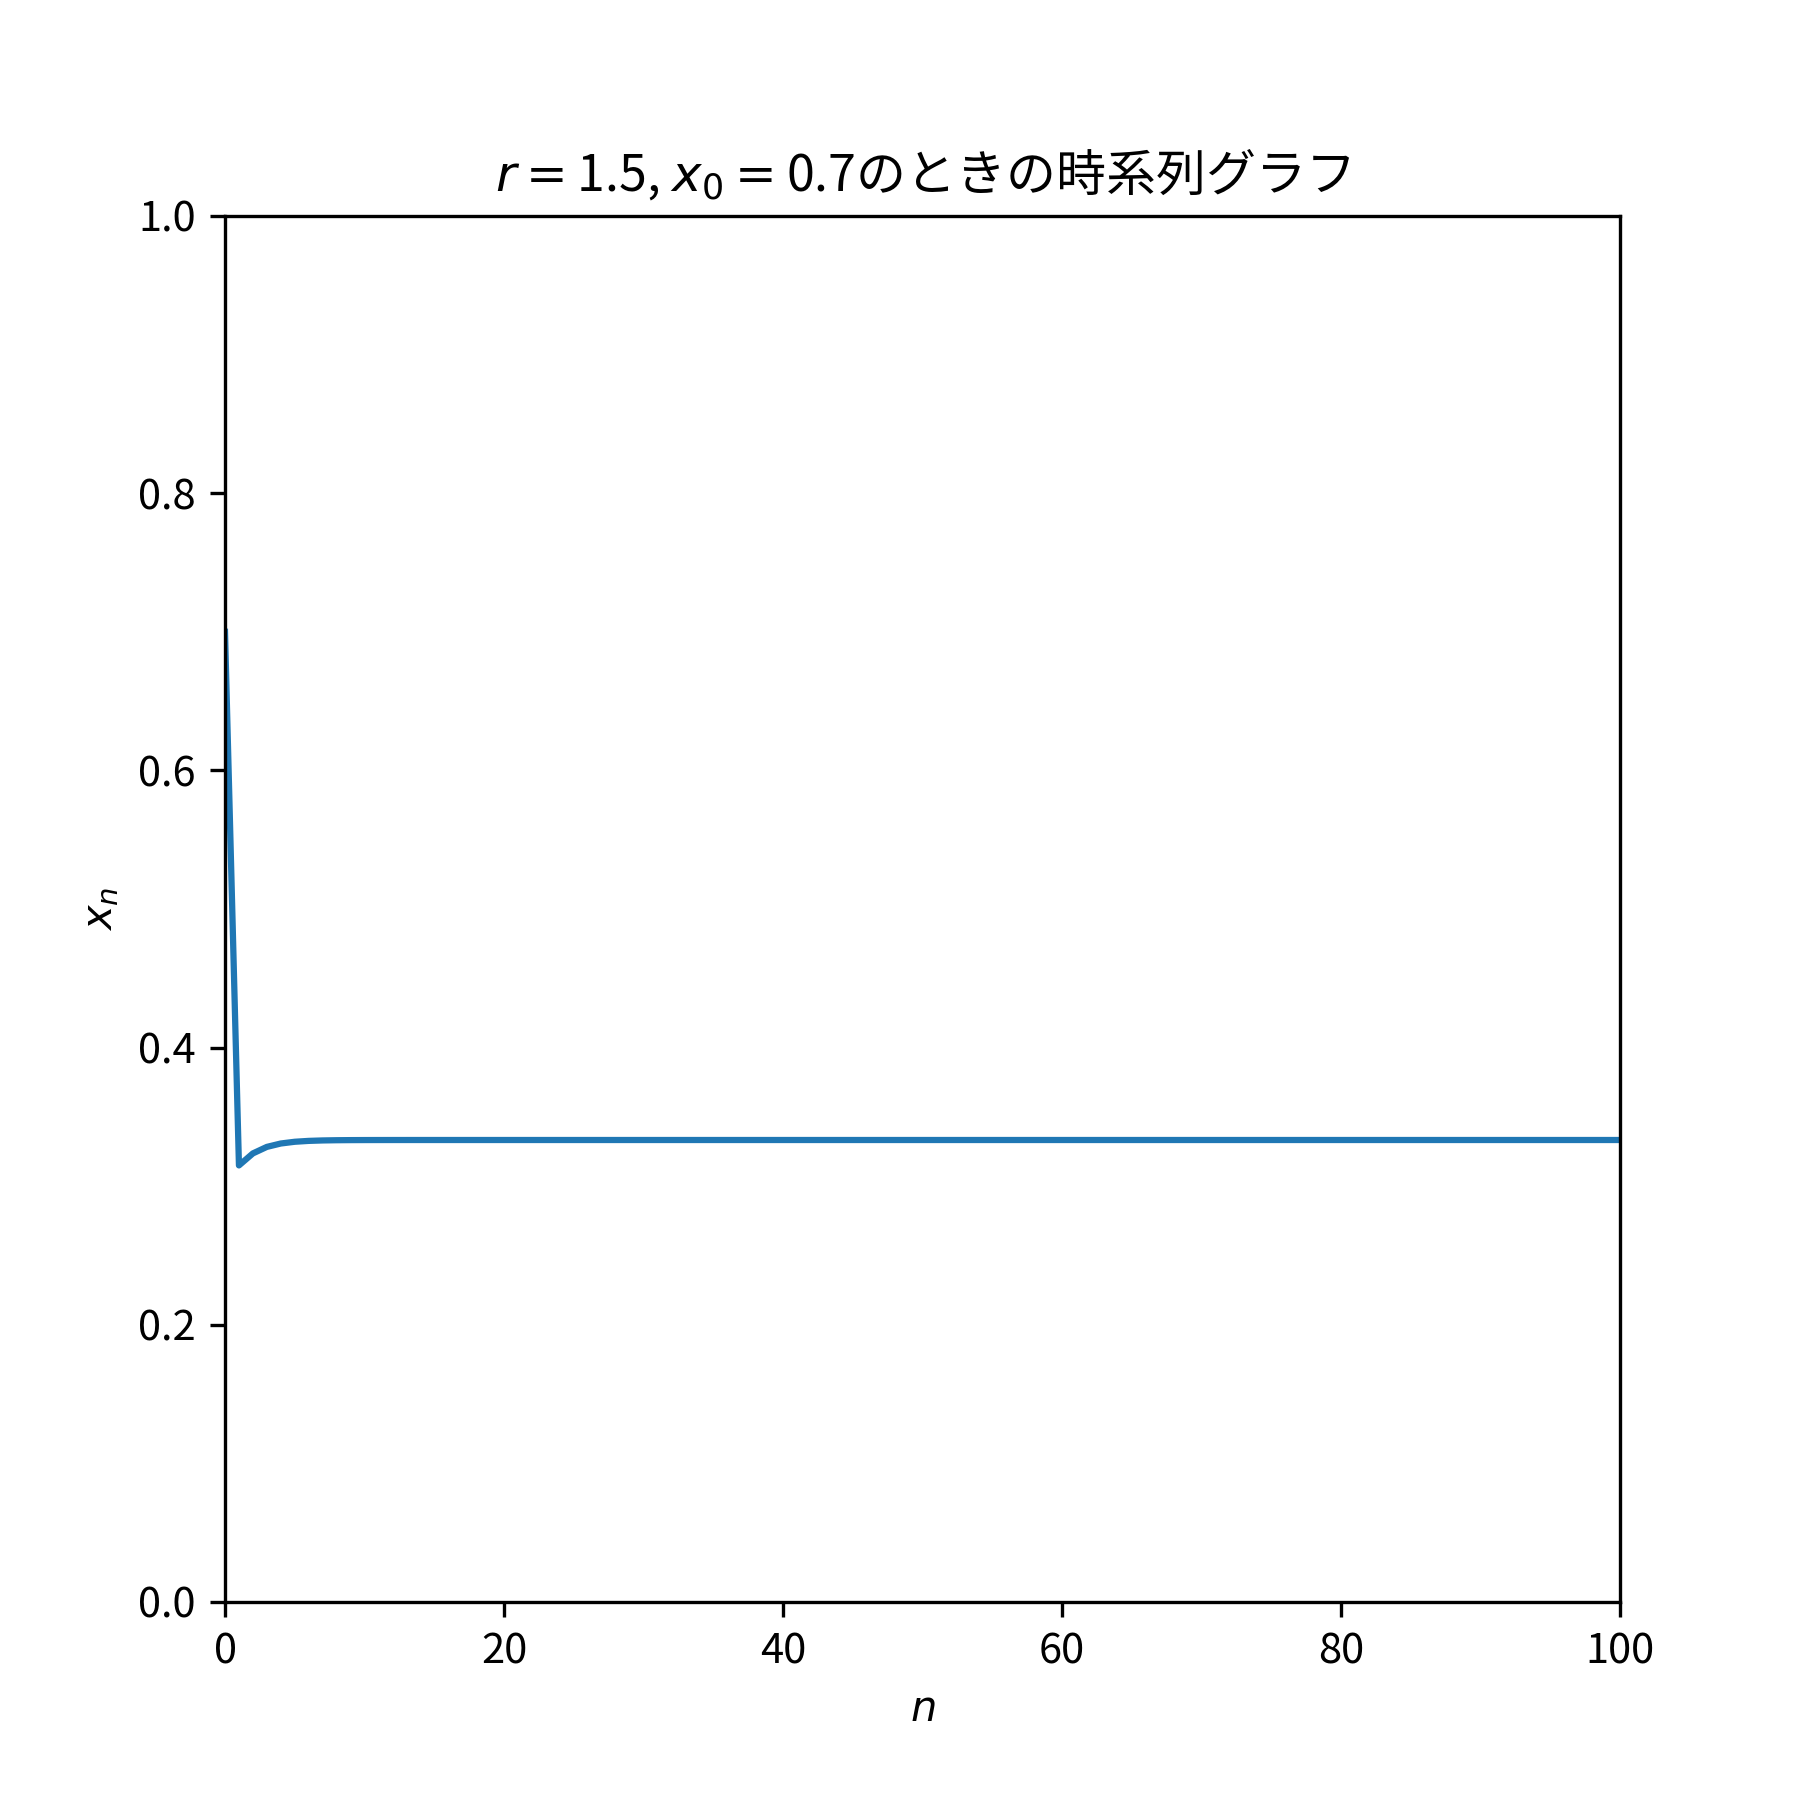
\includegraphics[keepaspectratio, scale=0.3]{images/Problem1/ctest2_1_1.png}
    \end{minipage} &
    \begin{minipage}[t]{0.45\hsize}
      \centering
      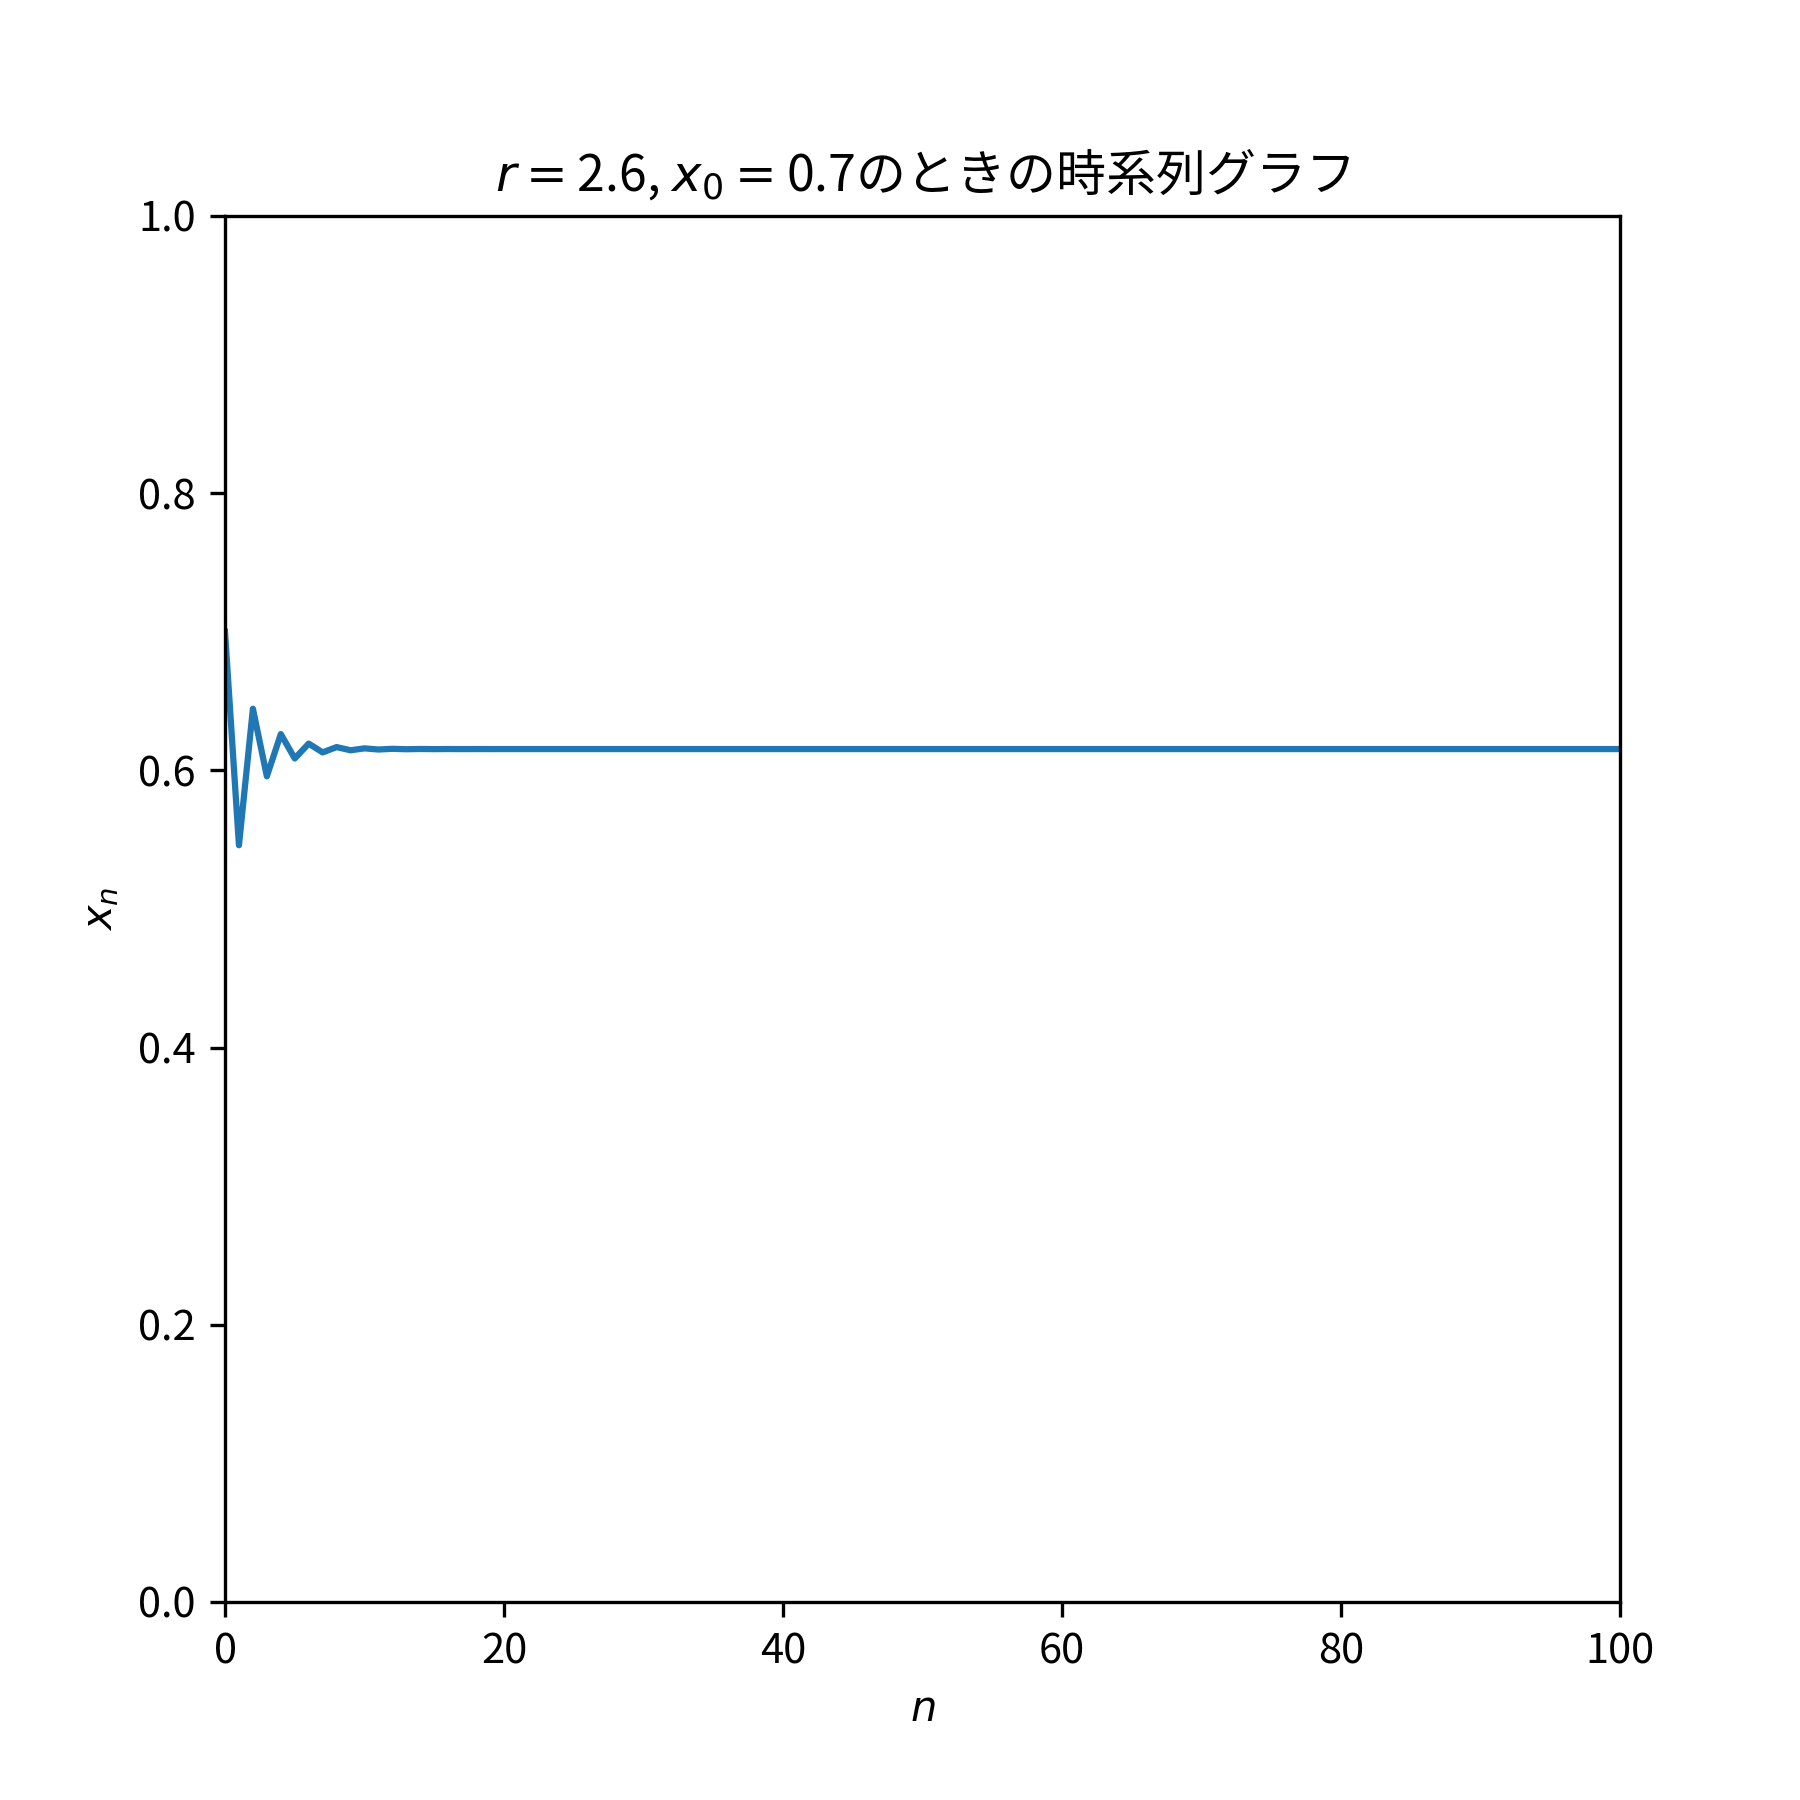
\includegraphics[keepaspectratio, scale=0.3]{images/Problem1/ctest2_2_1.png}
    \end{minipage} \\

    \begin{minipage}[t]{0.45\hsize}
      \centering
      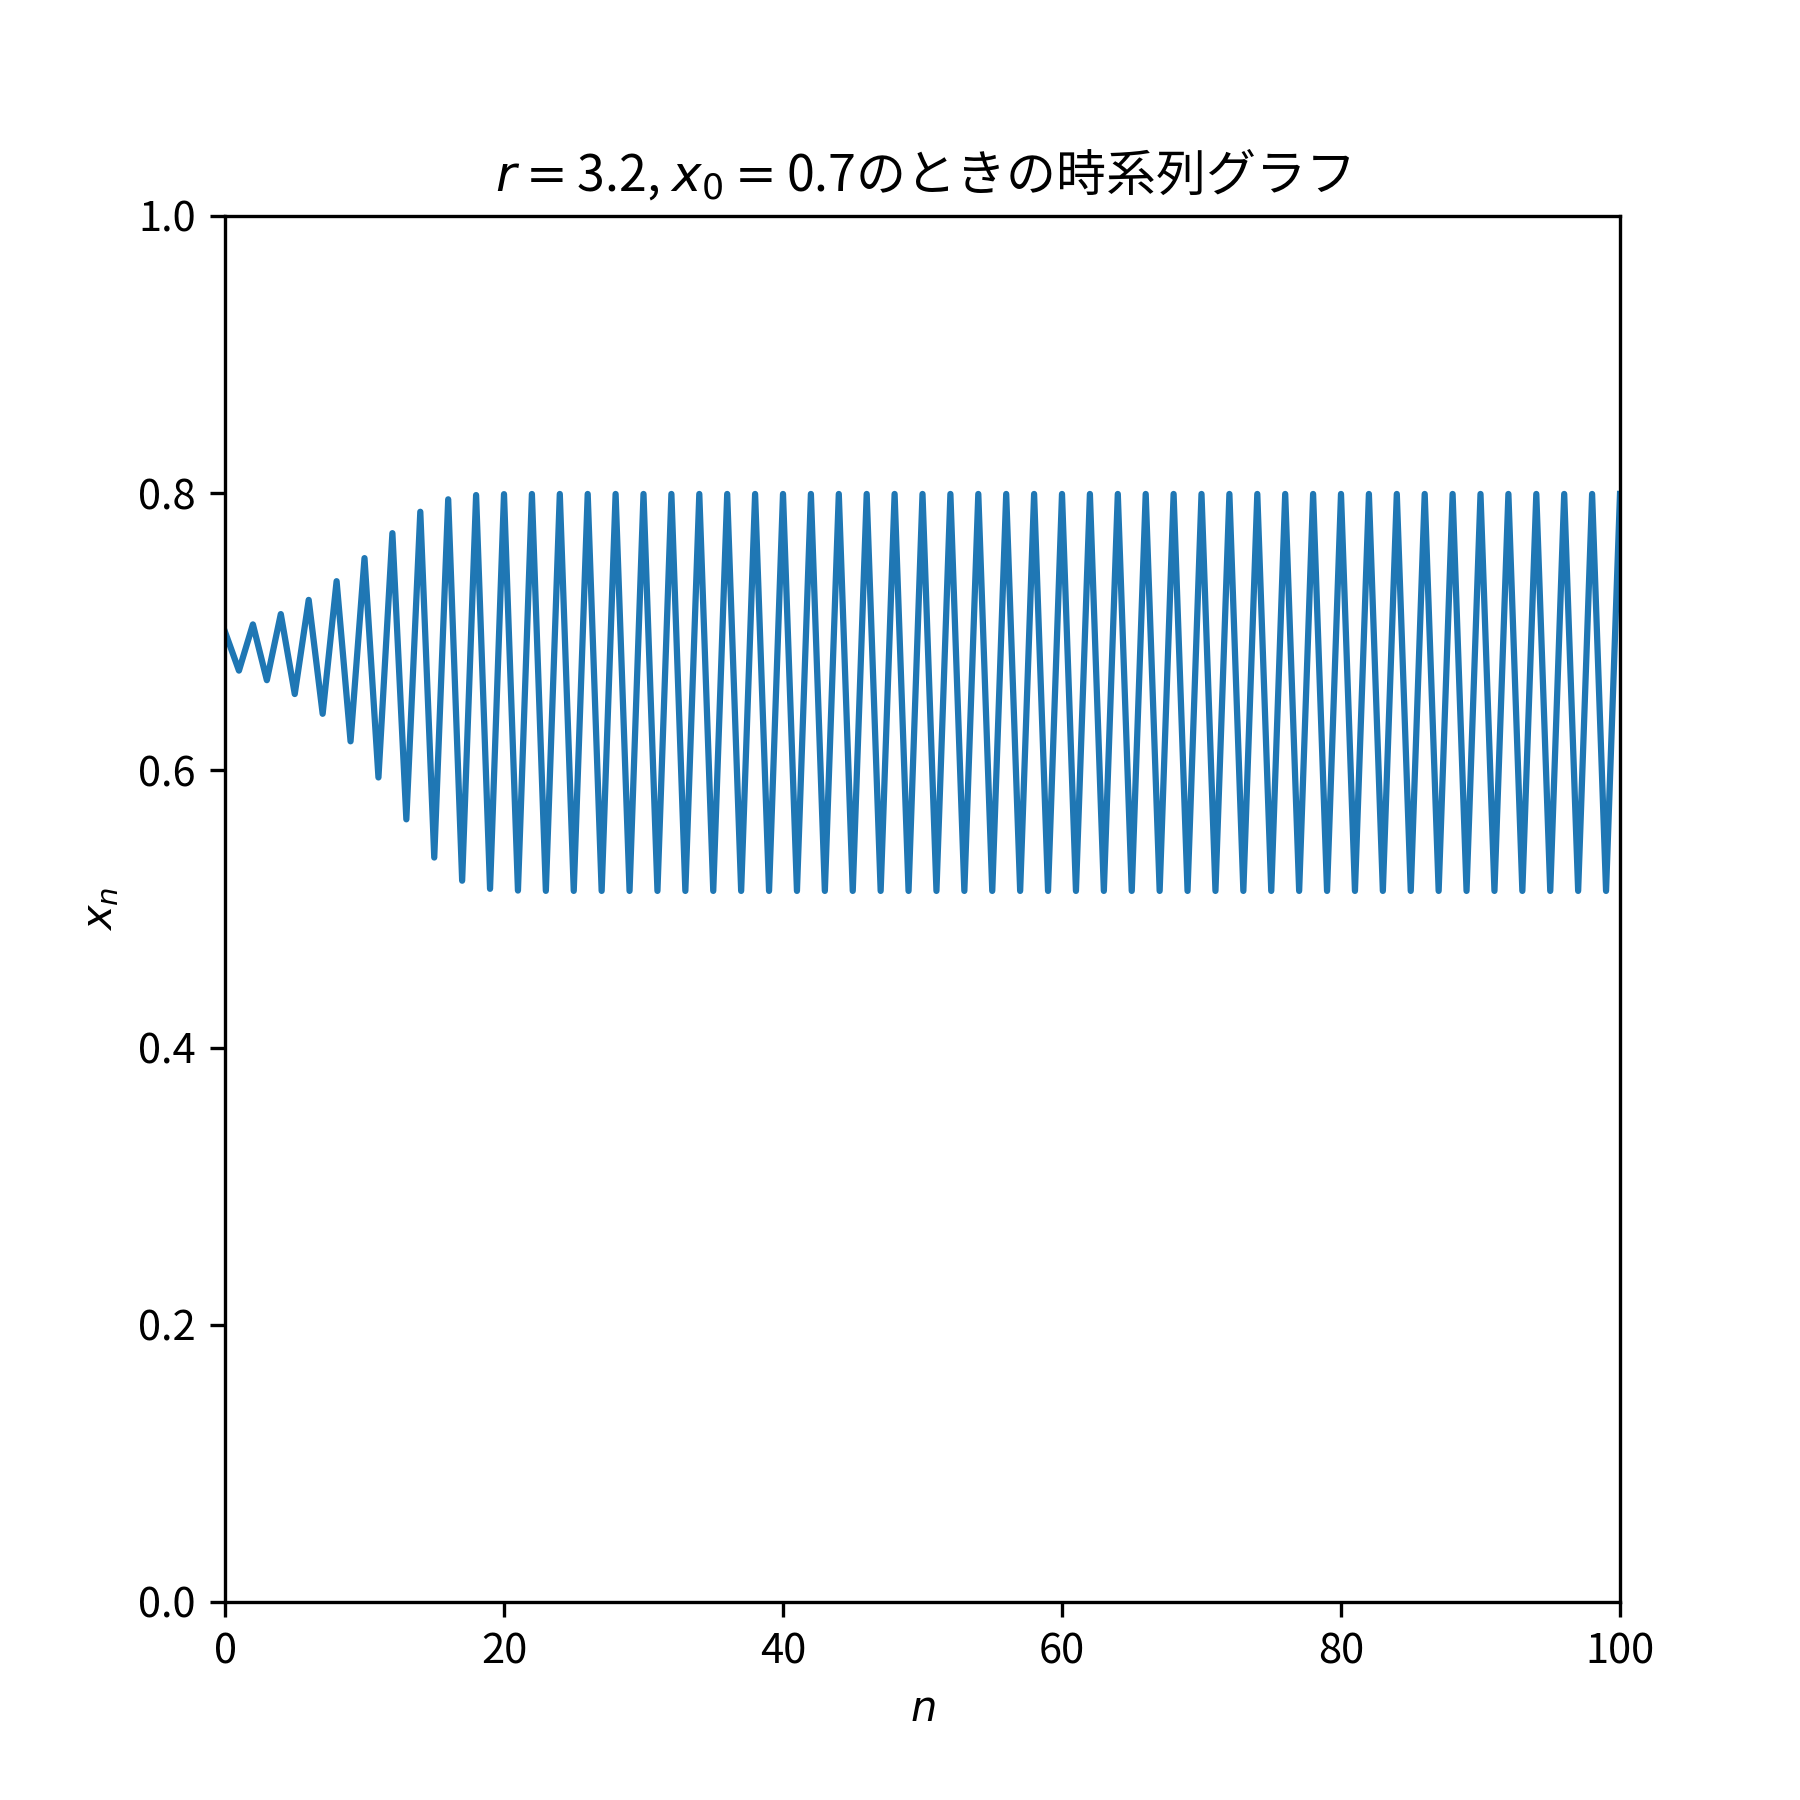
\includegraphics[keepaspectratio, scale=0.3]{images/Problem1/ctest2_3_1.png}
    \end{minipage} &
    \begin{minipage}[t]{0.45\hsize}
      \centering
      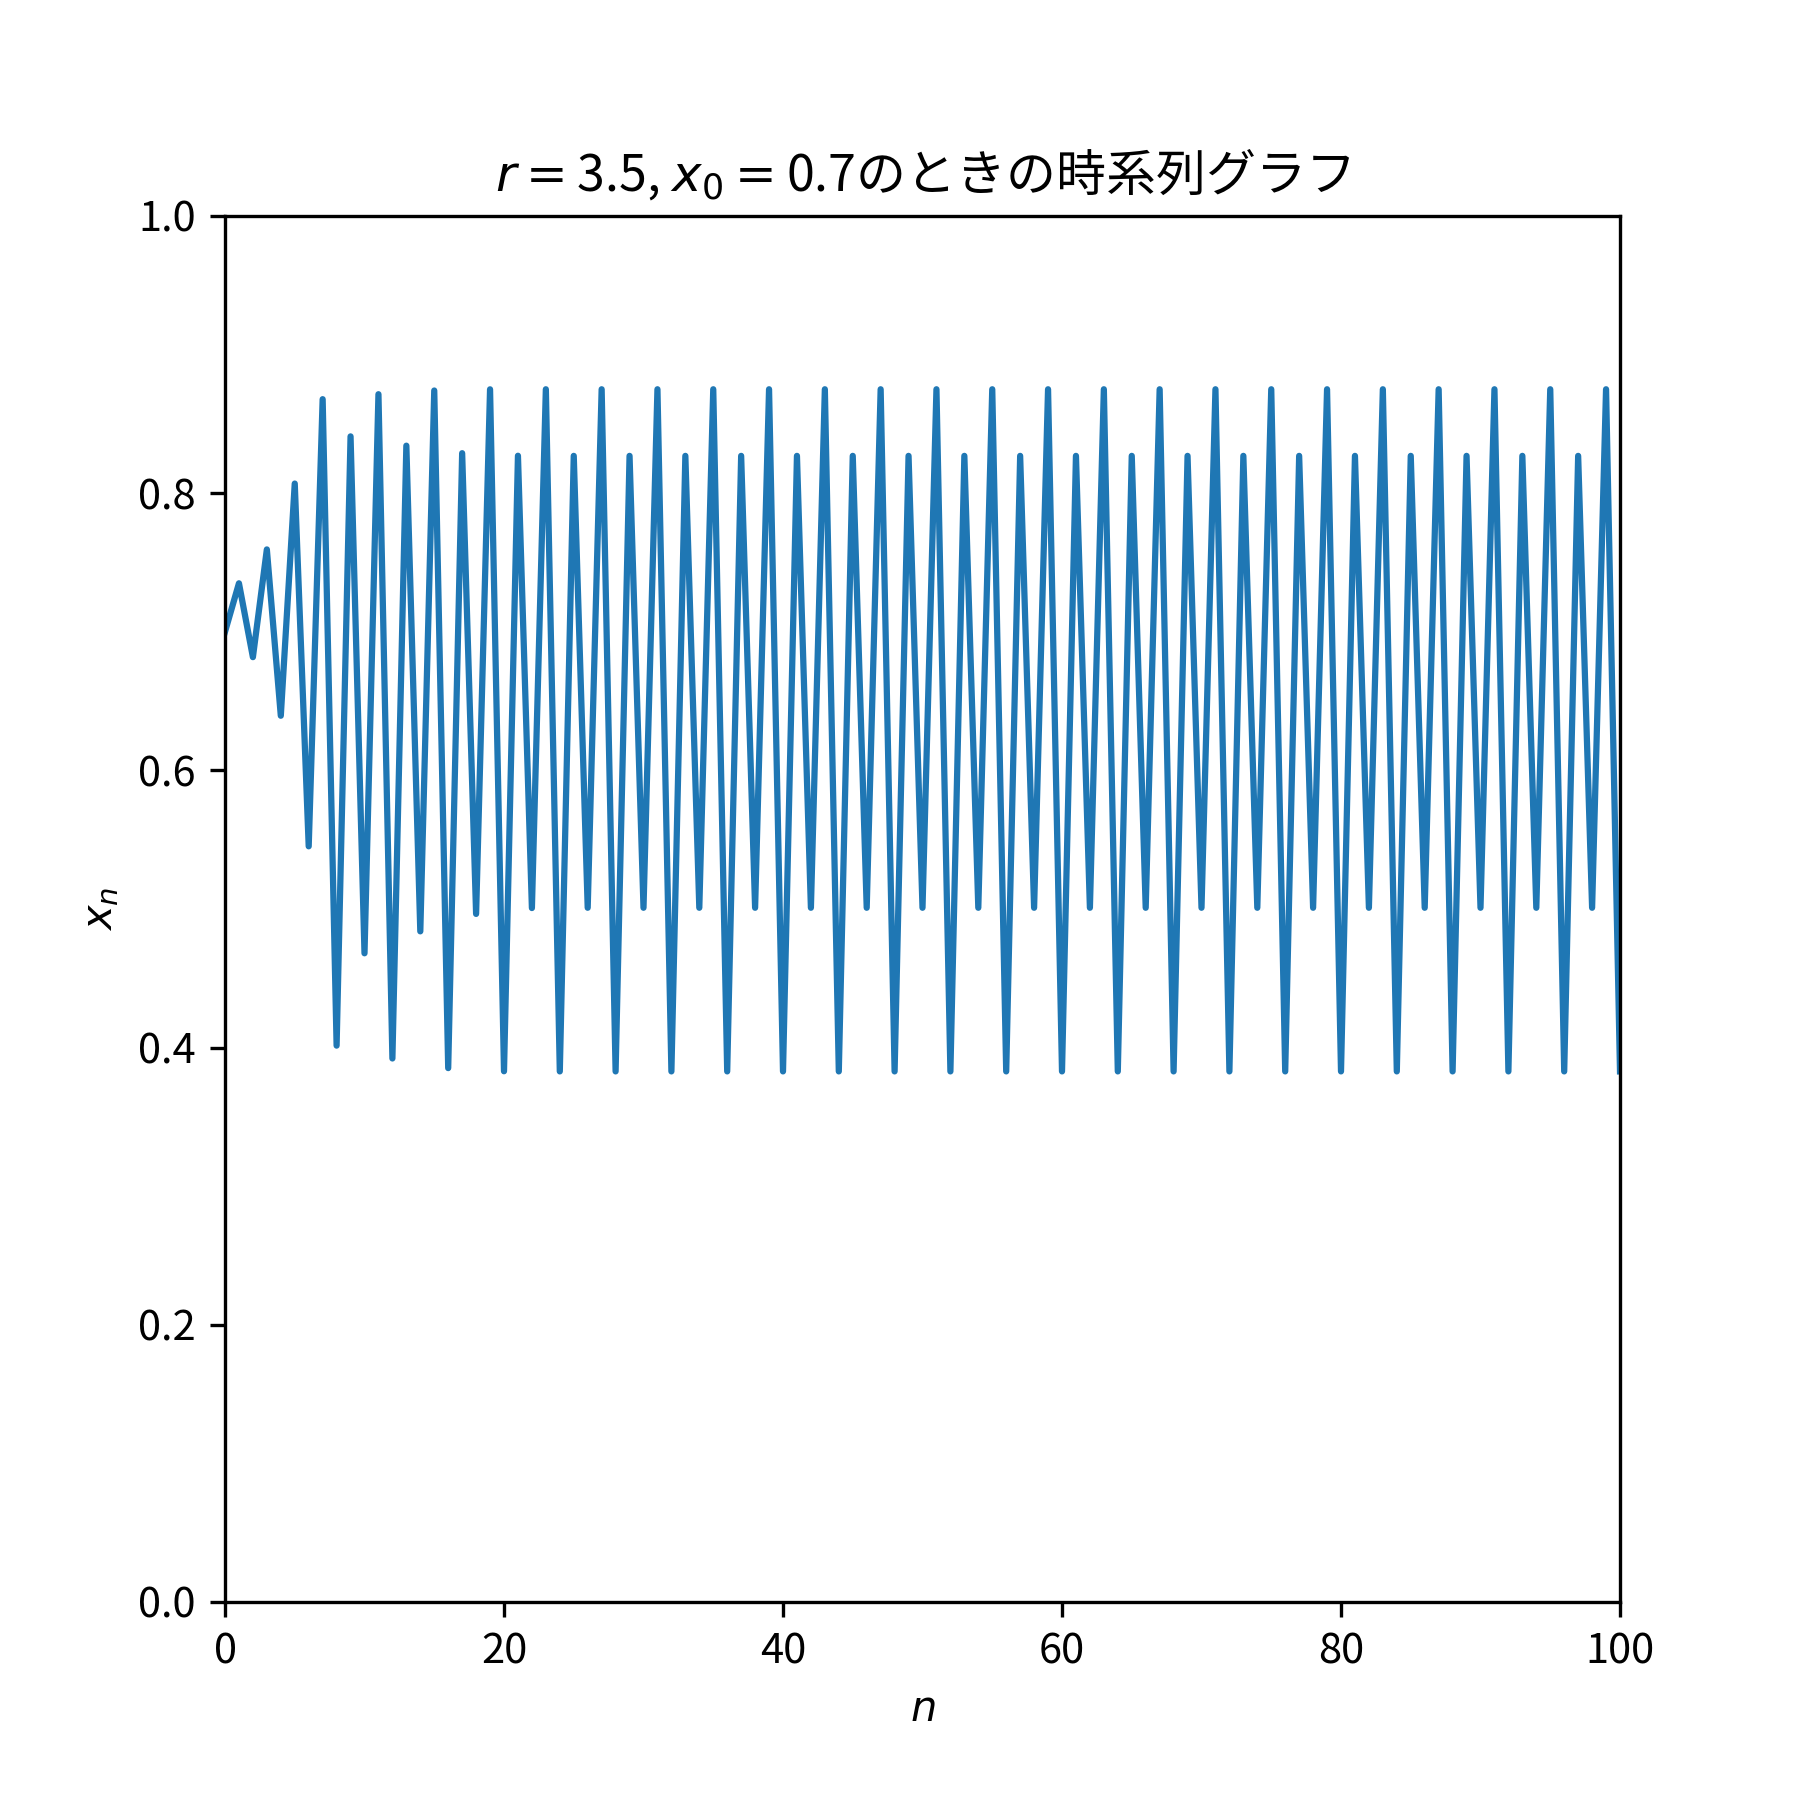
\includegraphics[keepaspectratio, scale=0.3]{images/Problem1/ctest2_4_1.png}
    \end{minipage} \\

    \begin{minipage}[t]{0.45\hsize}
      \centering
      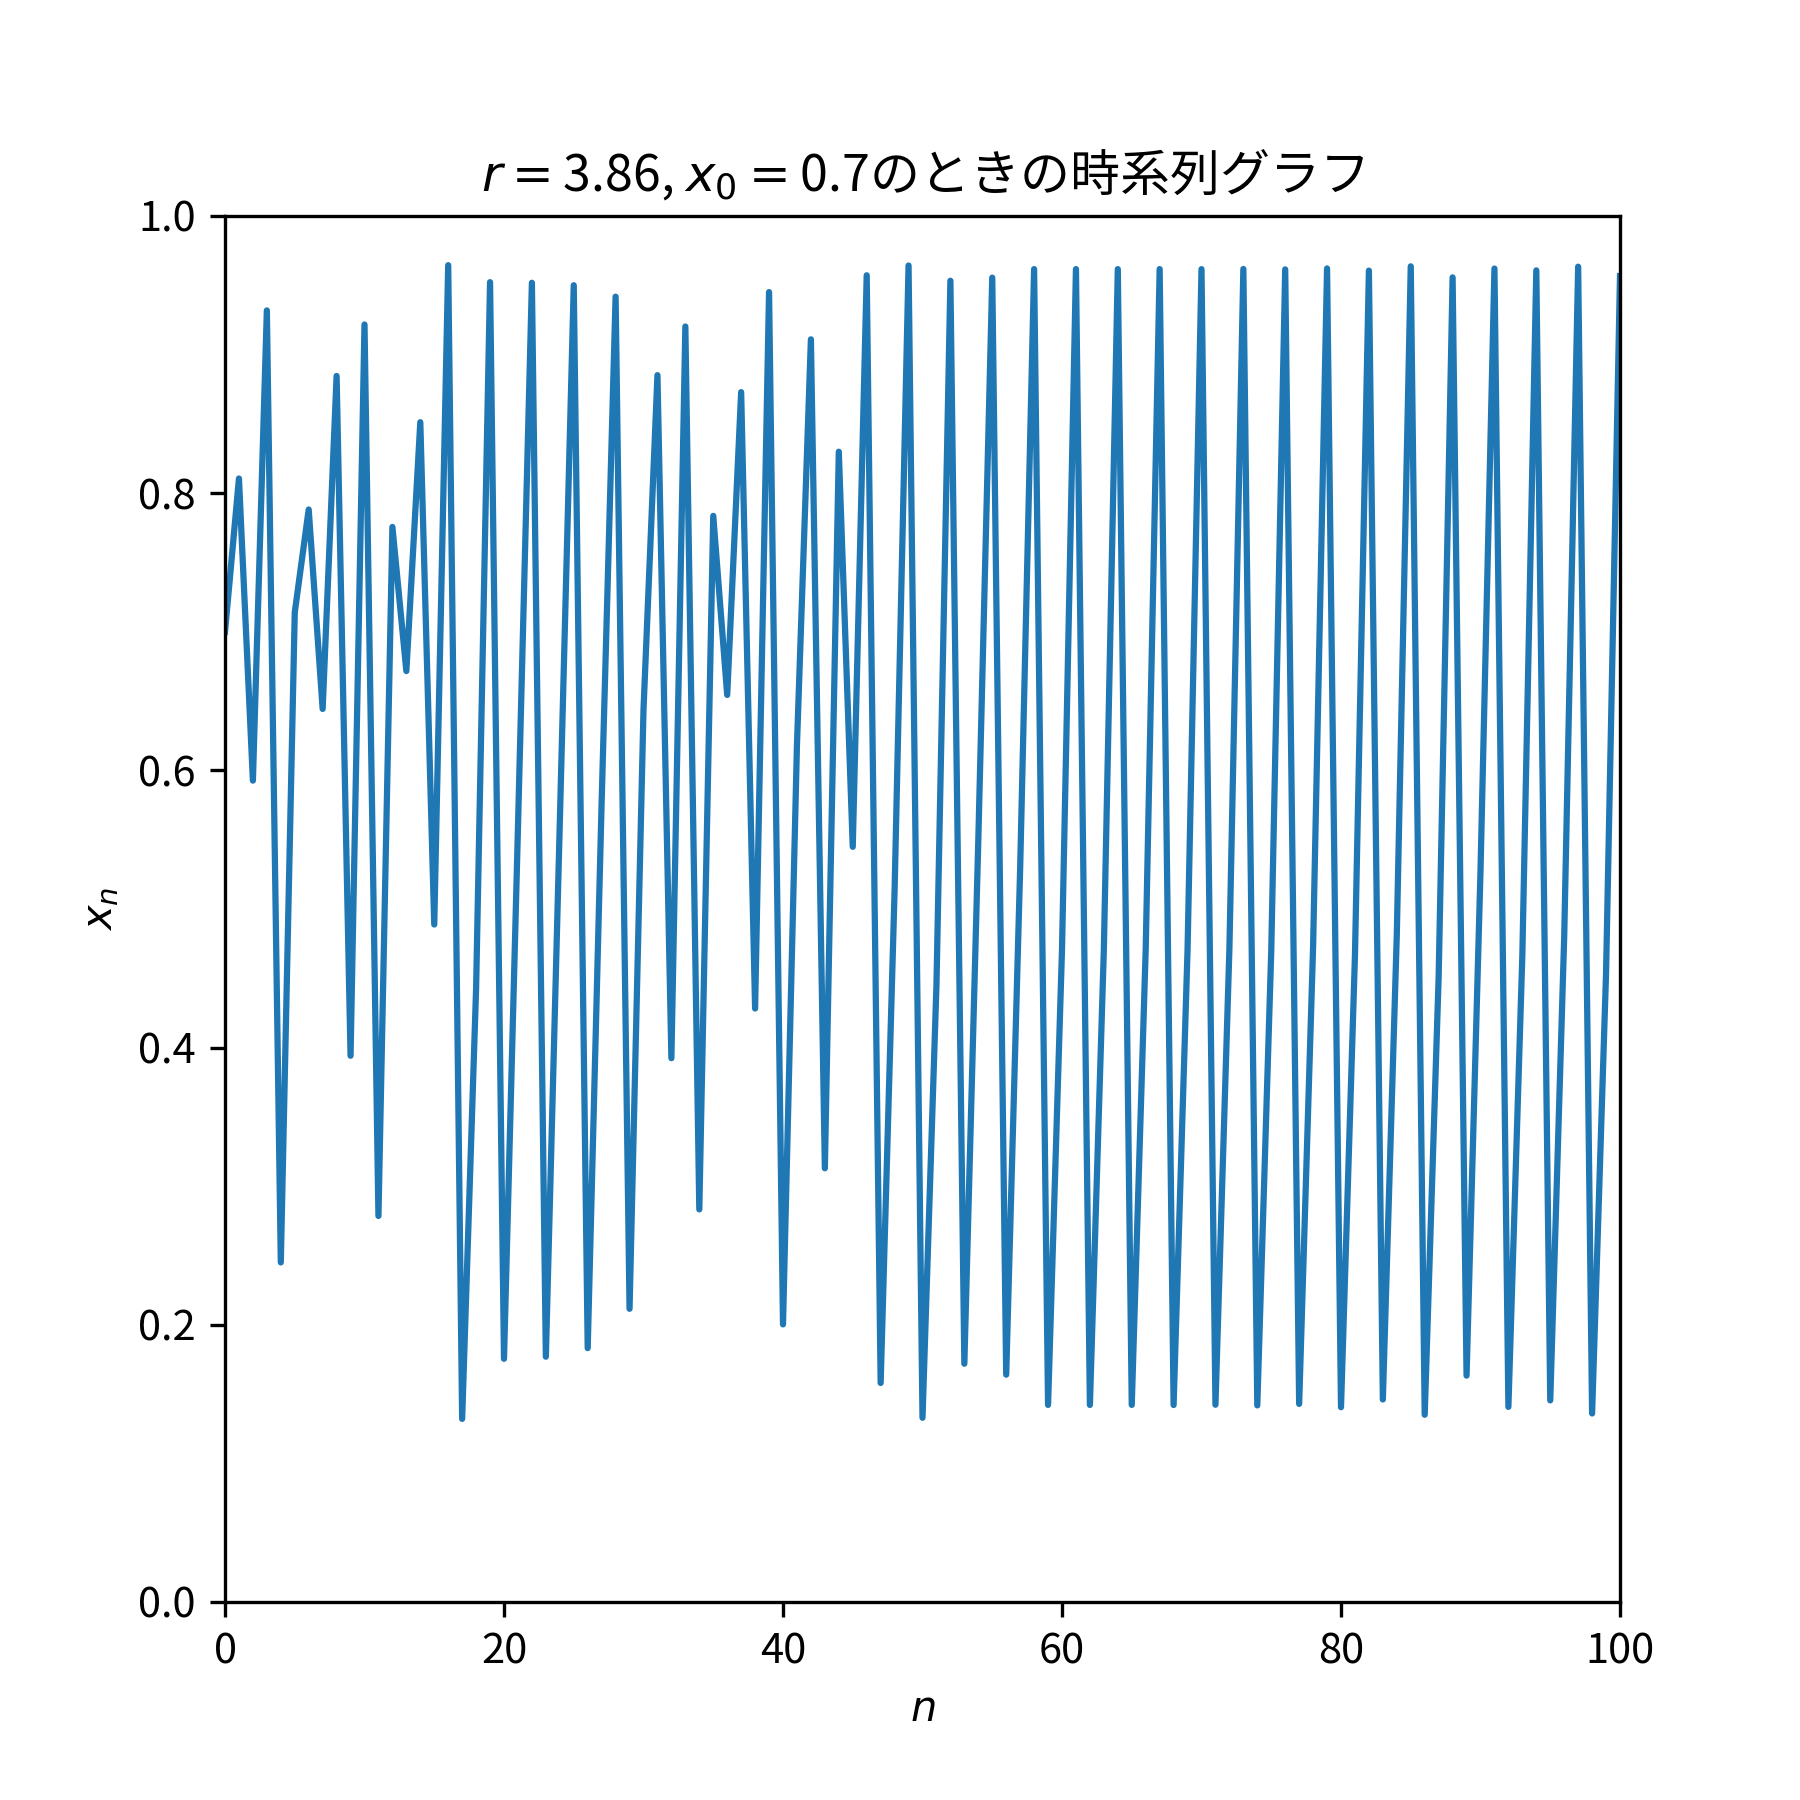
\includegraphics[keepaspectratio, scale=0.3]{images/Problem1/ctest2_5_1.png}
    \end{minipage} &
    \begin{minipage}[t]{0.45\hsize}
      \centering
      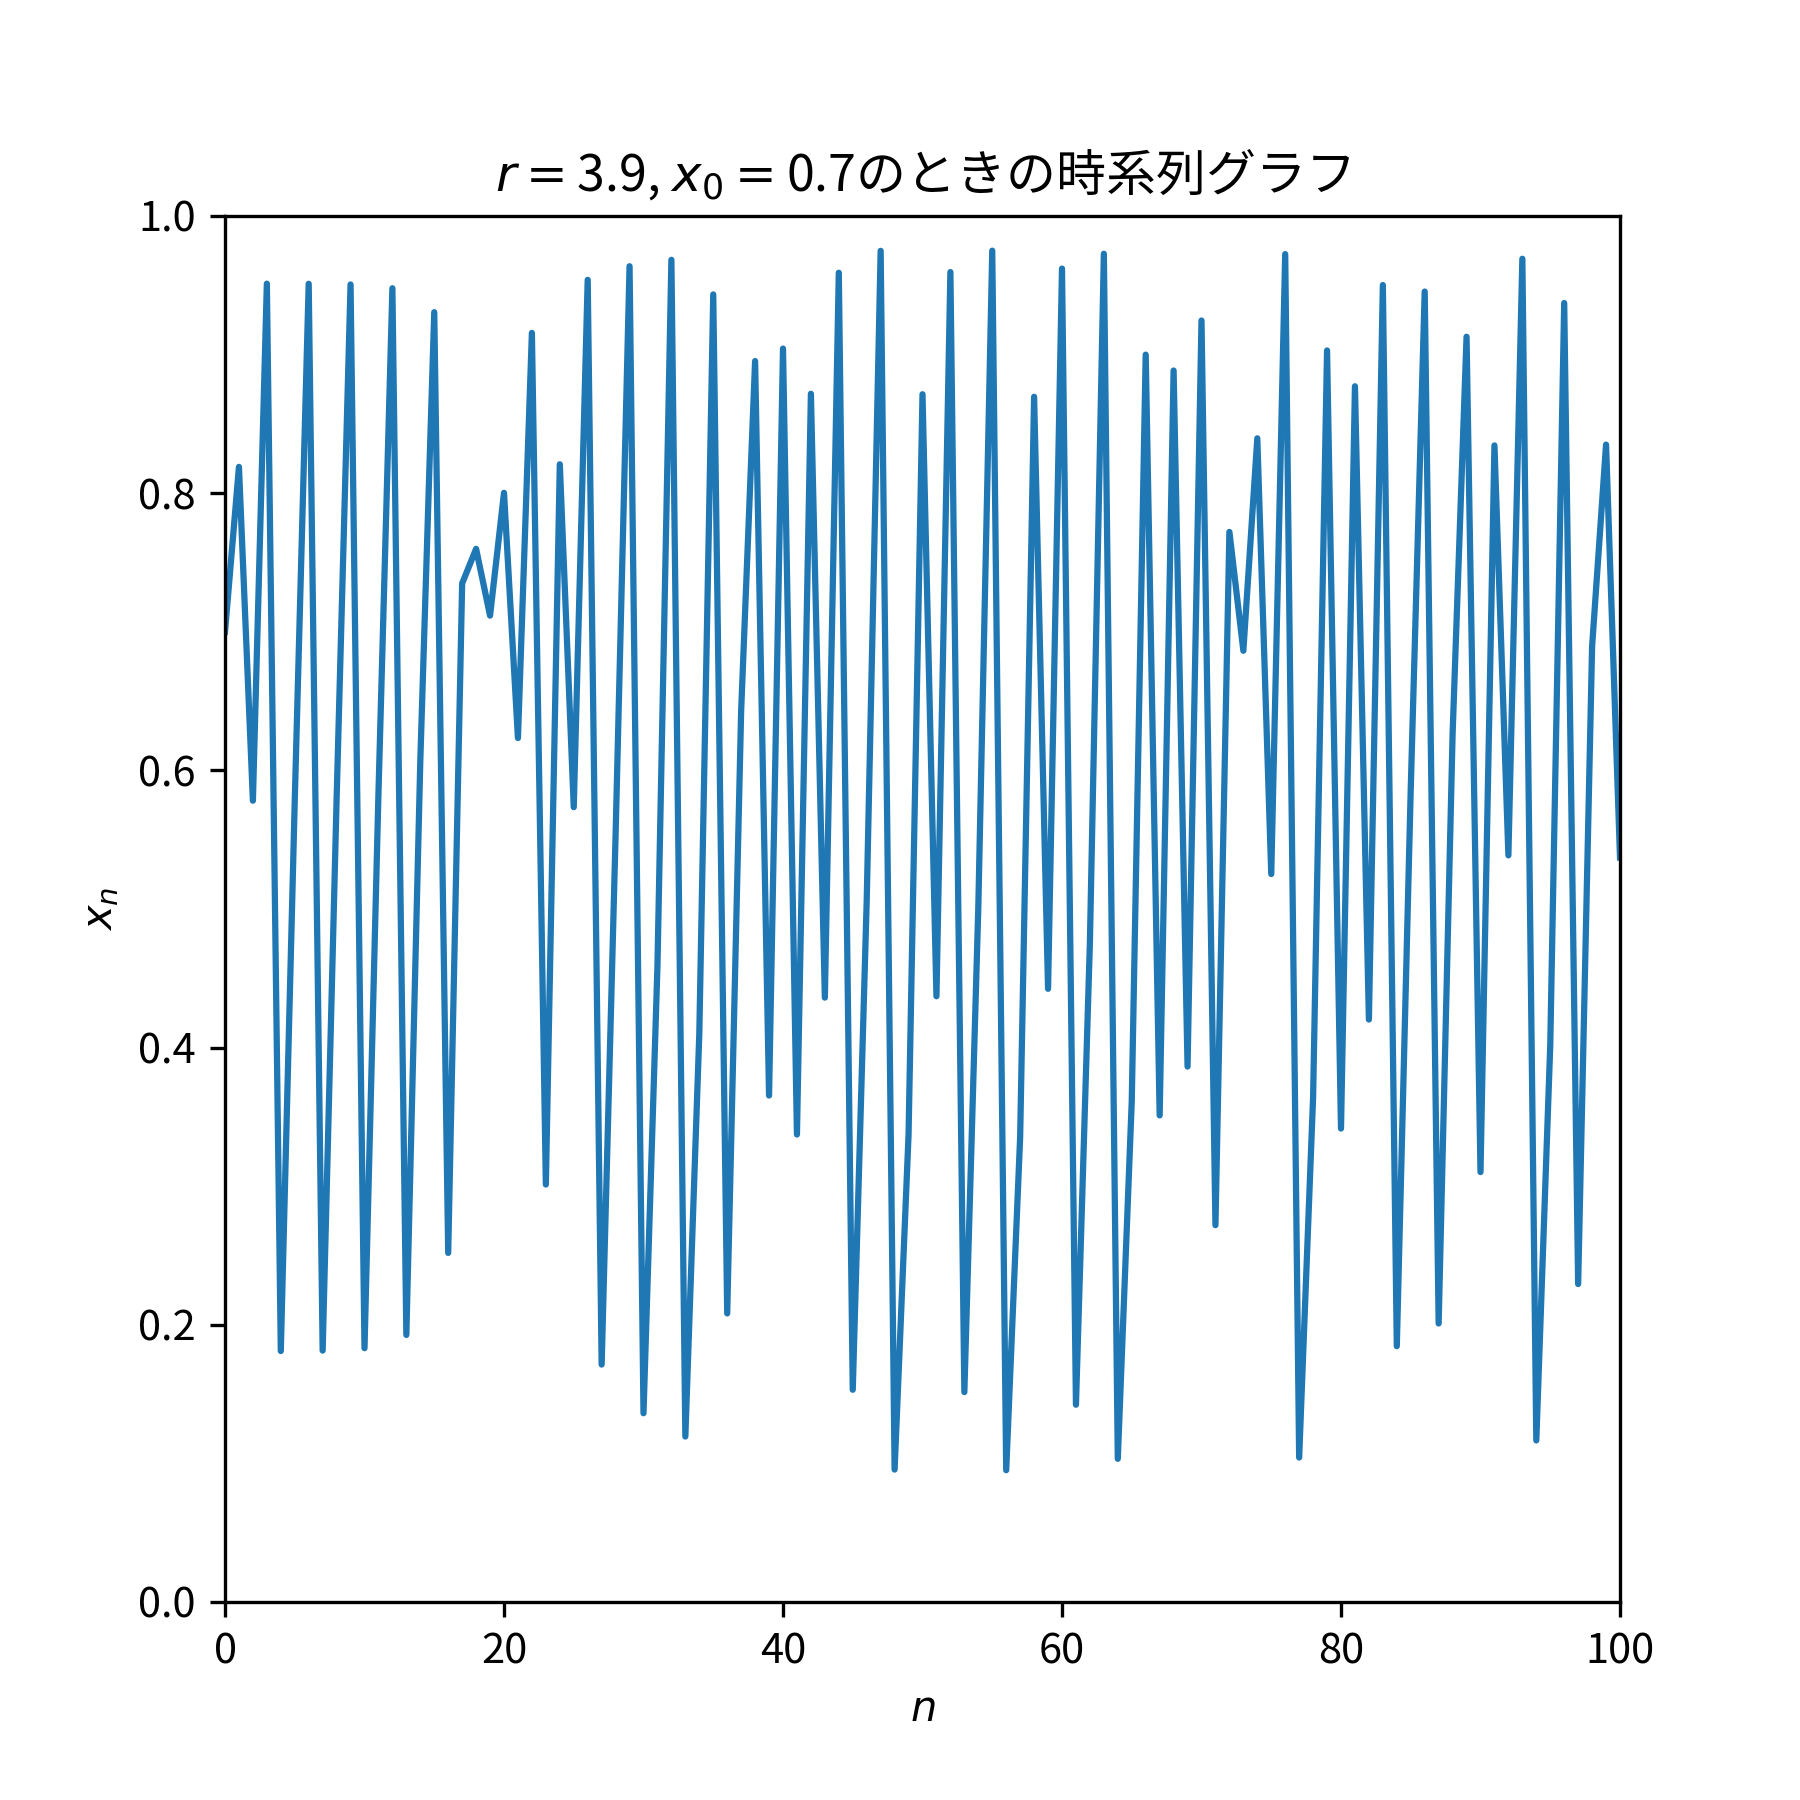
\includegraphics[keepaspectratio, scale=0.3]{images/Problem1/ctest2_6_1.png}
    \end{minipage}
  \end{tabular}
\end{figure}
結果:\\
時系列グラフは、ロジスティック回帰の各 $0 \leq n \leq 100$ のときの $x_n$ を計算しプロットしている。$x$ 軸は $n$ を、$y$ 軸には $x_n$ をとっている。この図から $r$ の値によって挙動が変わっているのが読み取れる。$r = 1.50, 2.60$ のときには $n$ を増加させていくと $x_n$ が収束していく。また、$r = 3.20, 3.50$ のときには $n$ を増加させていくと $x_n$ に周期性が見られるようになる。さらに、$r = 3.86, 3.90$ のときには $n$ を増加させていくと $x_n$ に周期性は現れることなく値が収束することもない。\\\\
考察:\\
この考察から、ロジスティック回帰は $r$ の値を変化させていくことでカオスの条件を満たす場合と満たさない場合があると考察した。\\


\subsection{課題2}
ロジスティク写像のリターンマップを描くためのプログラムを作成し、$r = 1.50, r = 2.60, r = 3.20,$ \\
$r = 3.50, r = 3.86, r = 3.90 のとき、x0 = 0.7$として個体数変動のリターンマッ
プを表示せよ。グラフには、$x_{n+1} = r(1 −x_n)x_n とx_{n+1} = x_n$ のグラフも表示すること。\\
画像:\\
\begin{figure}[htbp]
  \begin{tabular}{cc}
    \begin{minipage}[t]{0.45\hsize}
      \centering
      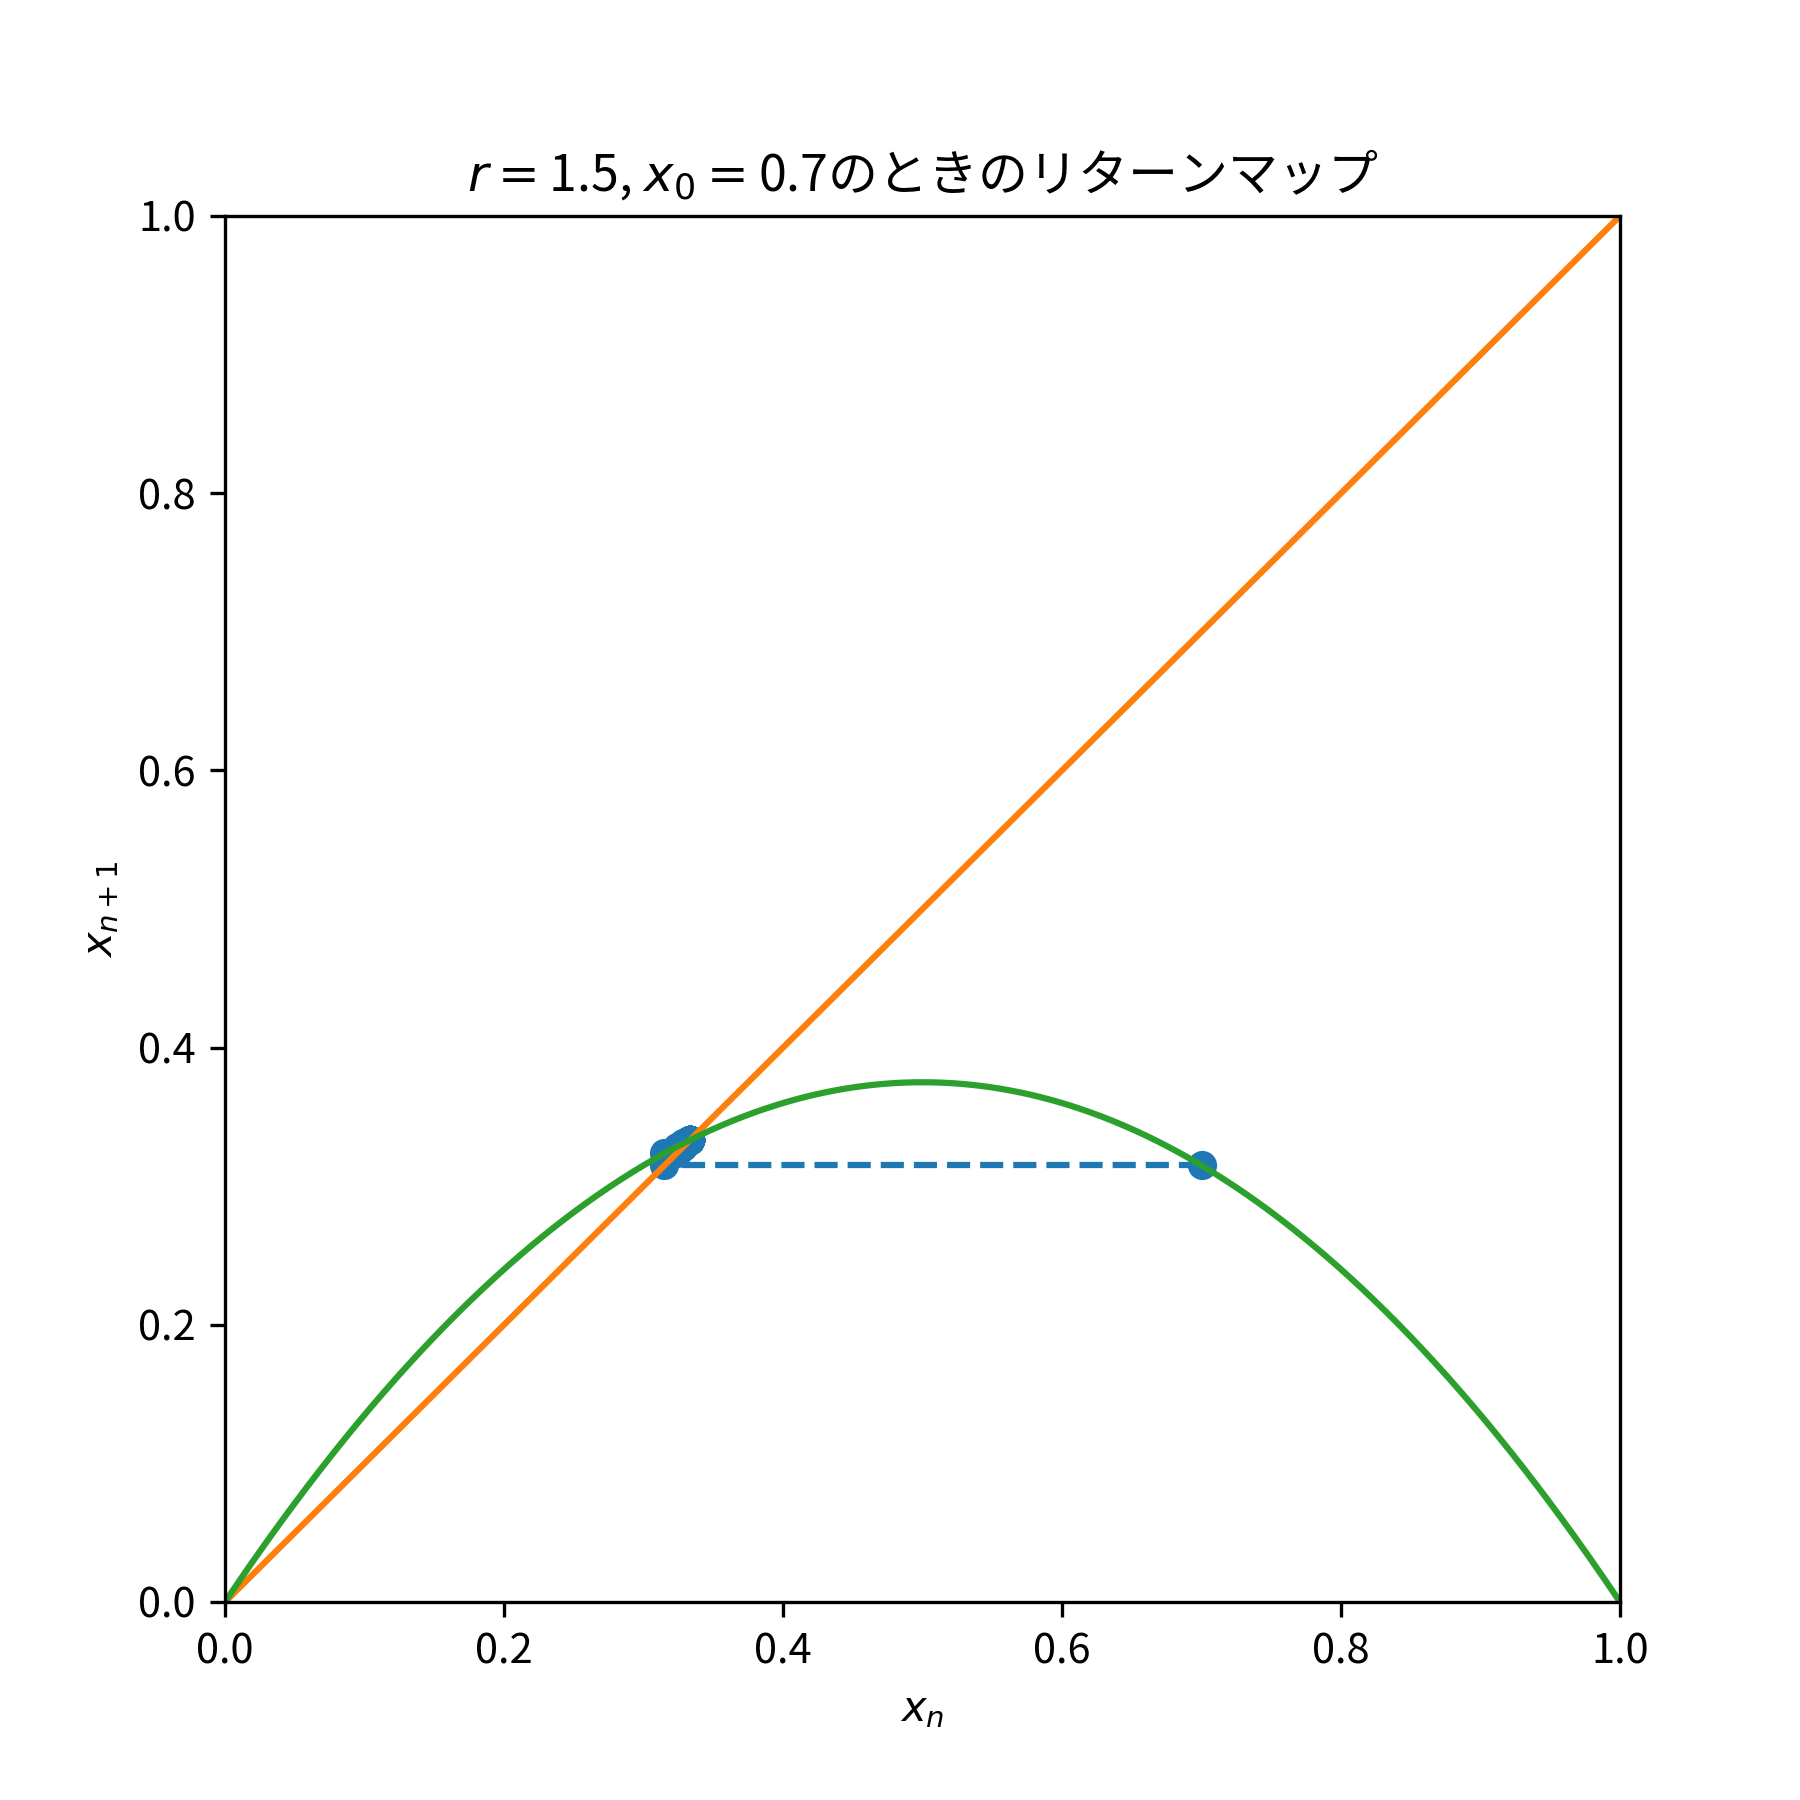
\includegraphics[keepaspectratio, scale=0.3]{images/Problem1/ctest2_1_2.png}
    \end{minipage} &
    \begin{minipage}[t]{0.45\hsize}
      \centering
      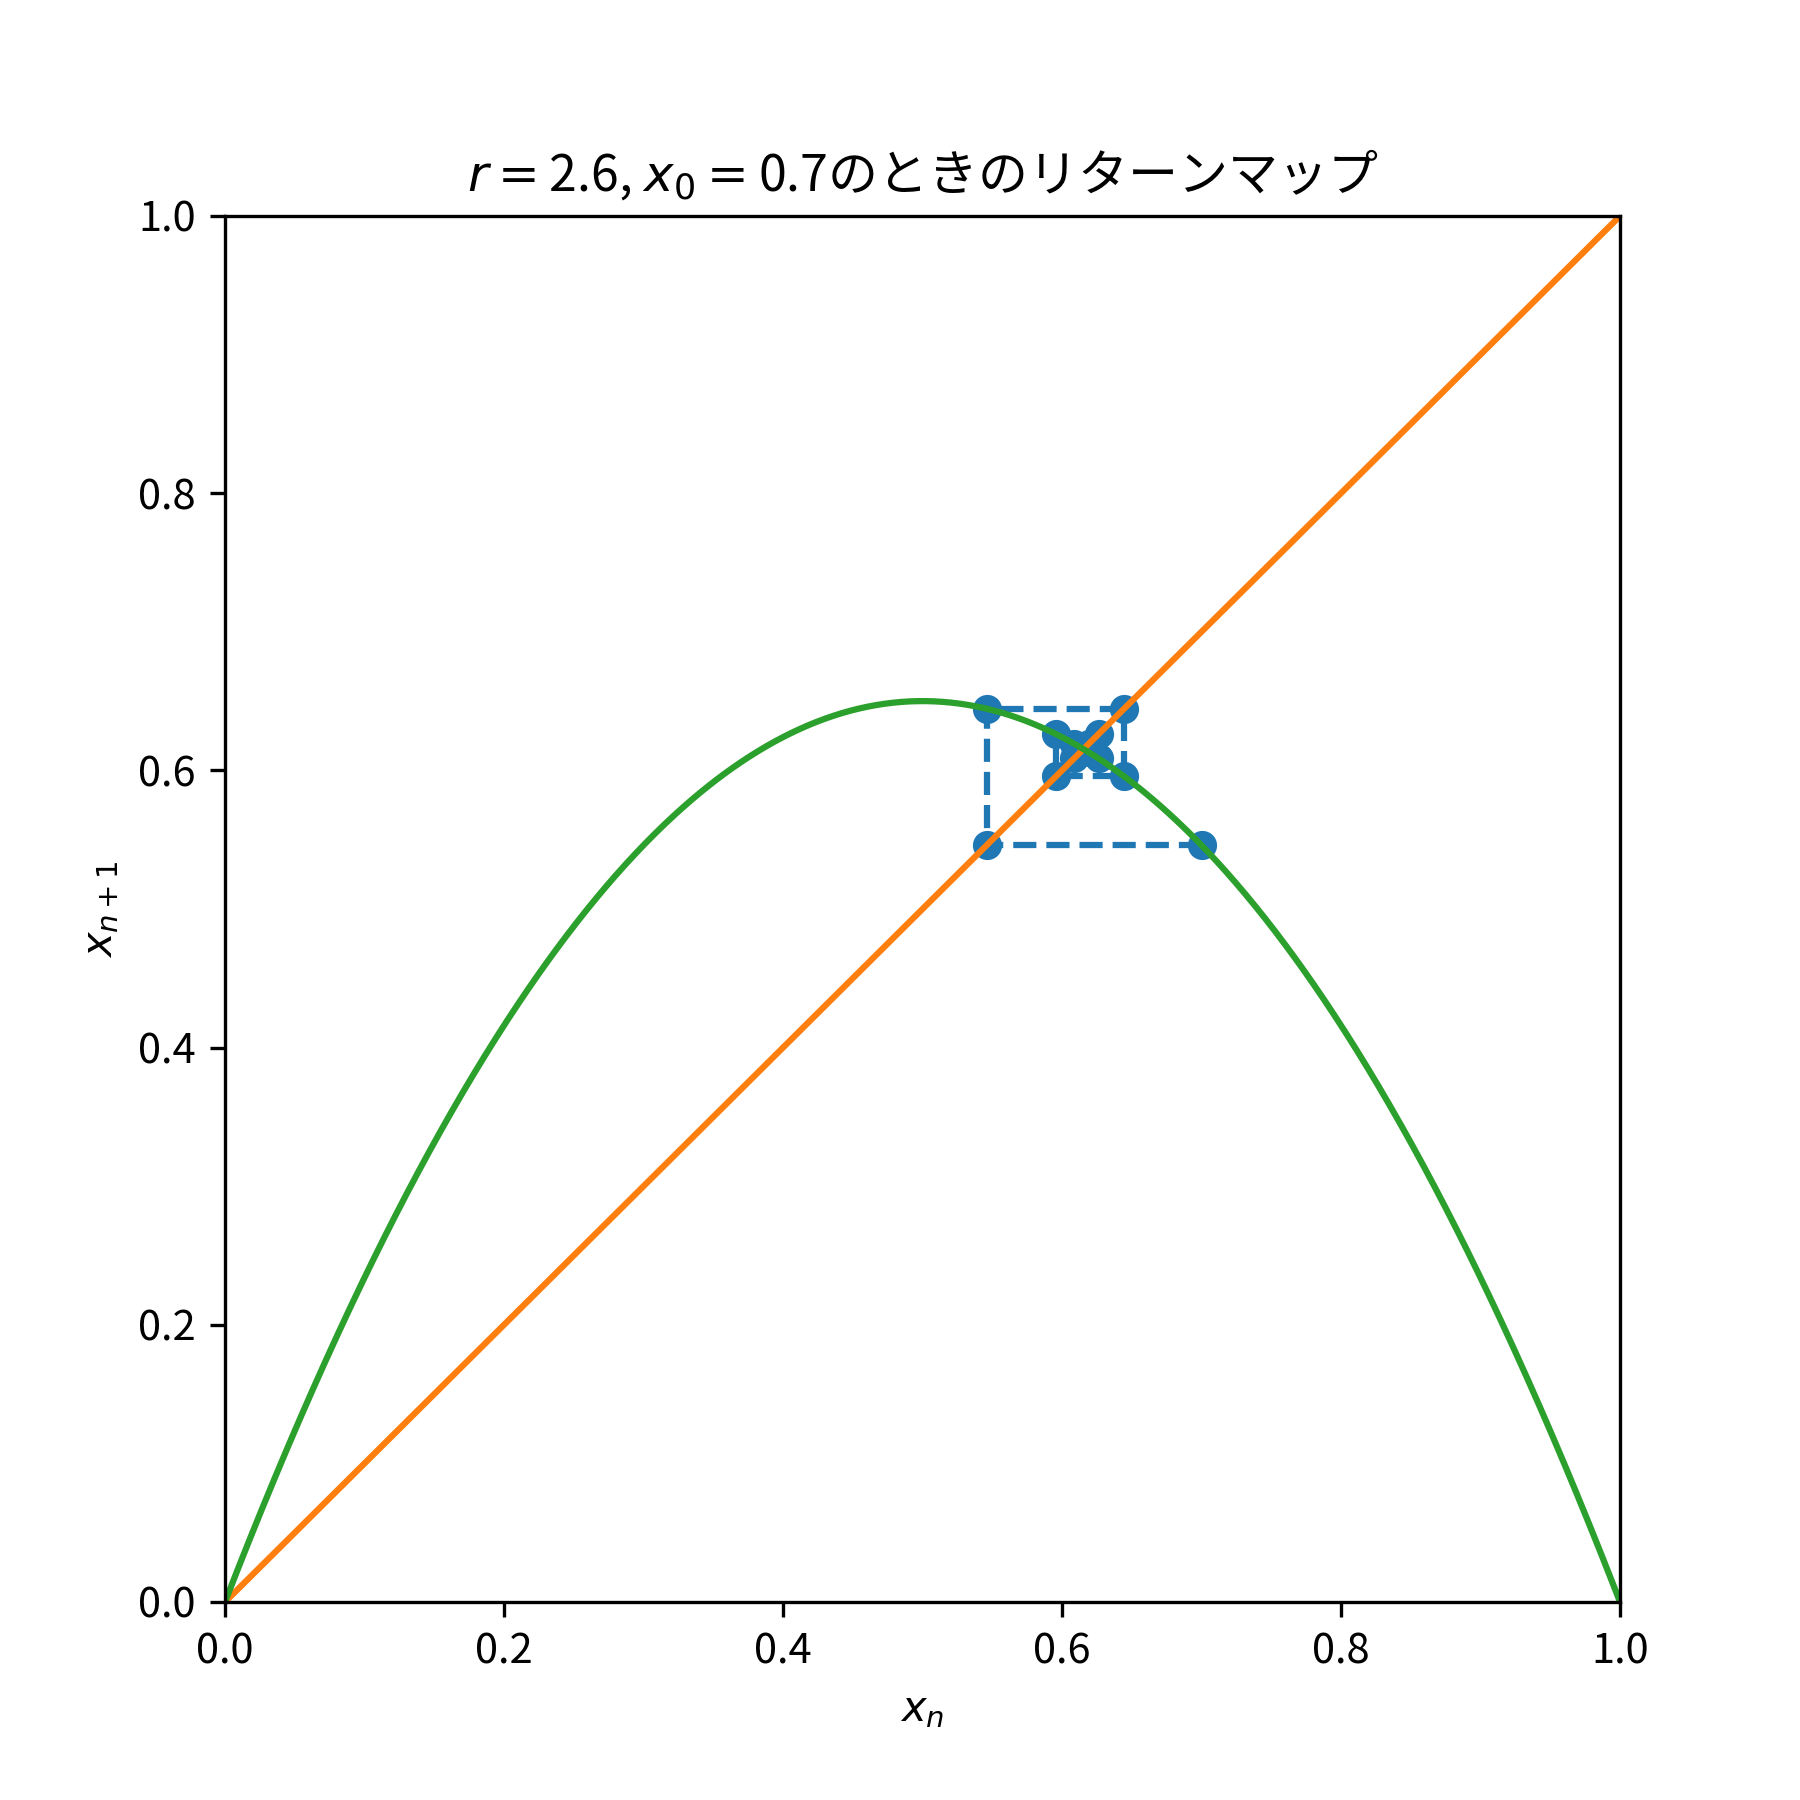
\includegraphics[keepaspectratio, scale=0.3]{images/Problem1/ctest2_2_2.png}
    \end{minipage} \\

    \begin{minipage}[t]{0.45\hsize}
      \centering
      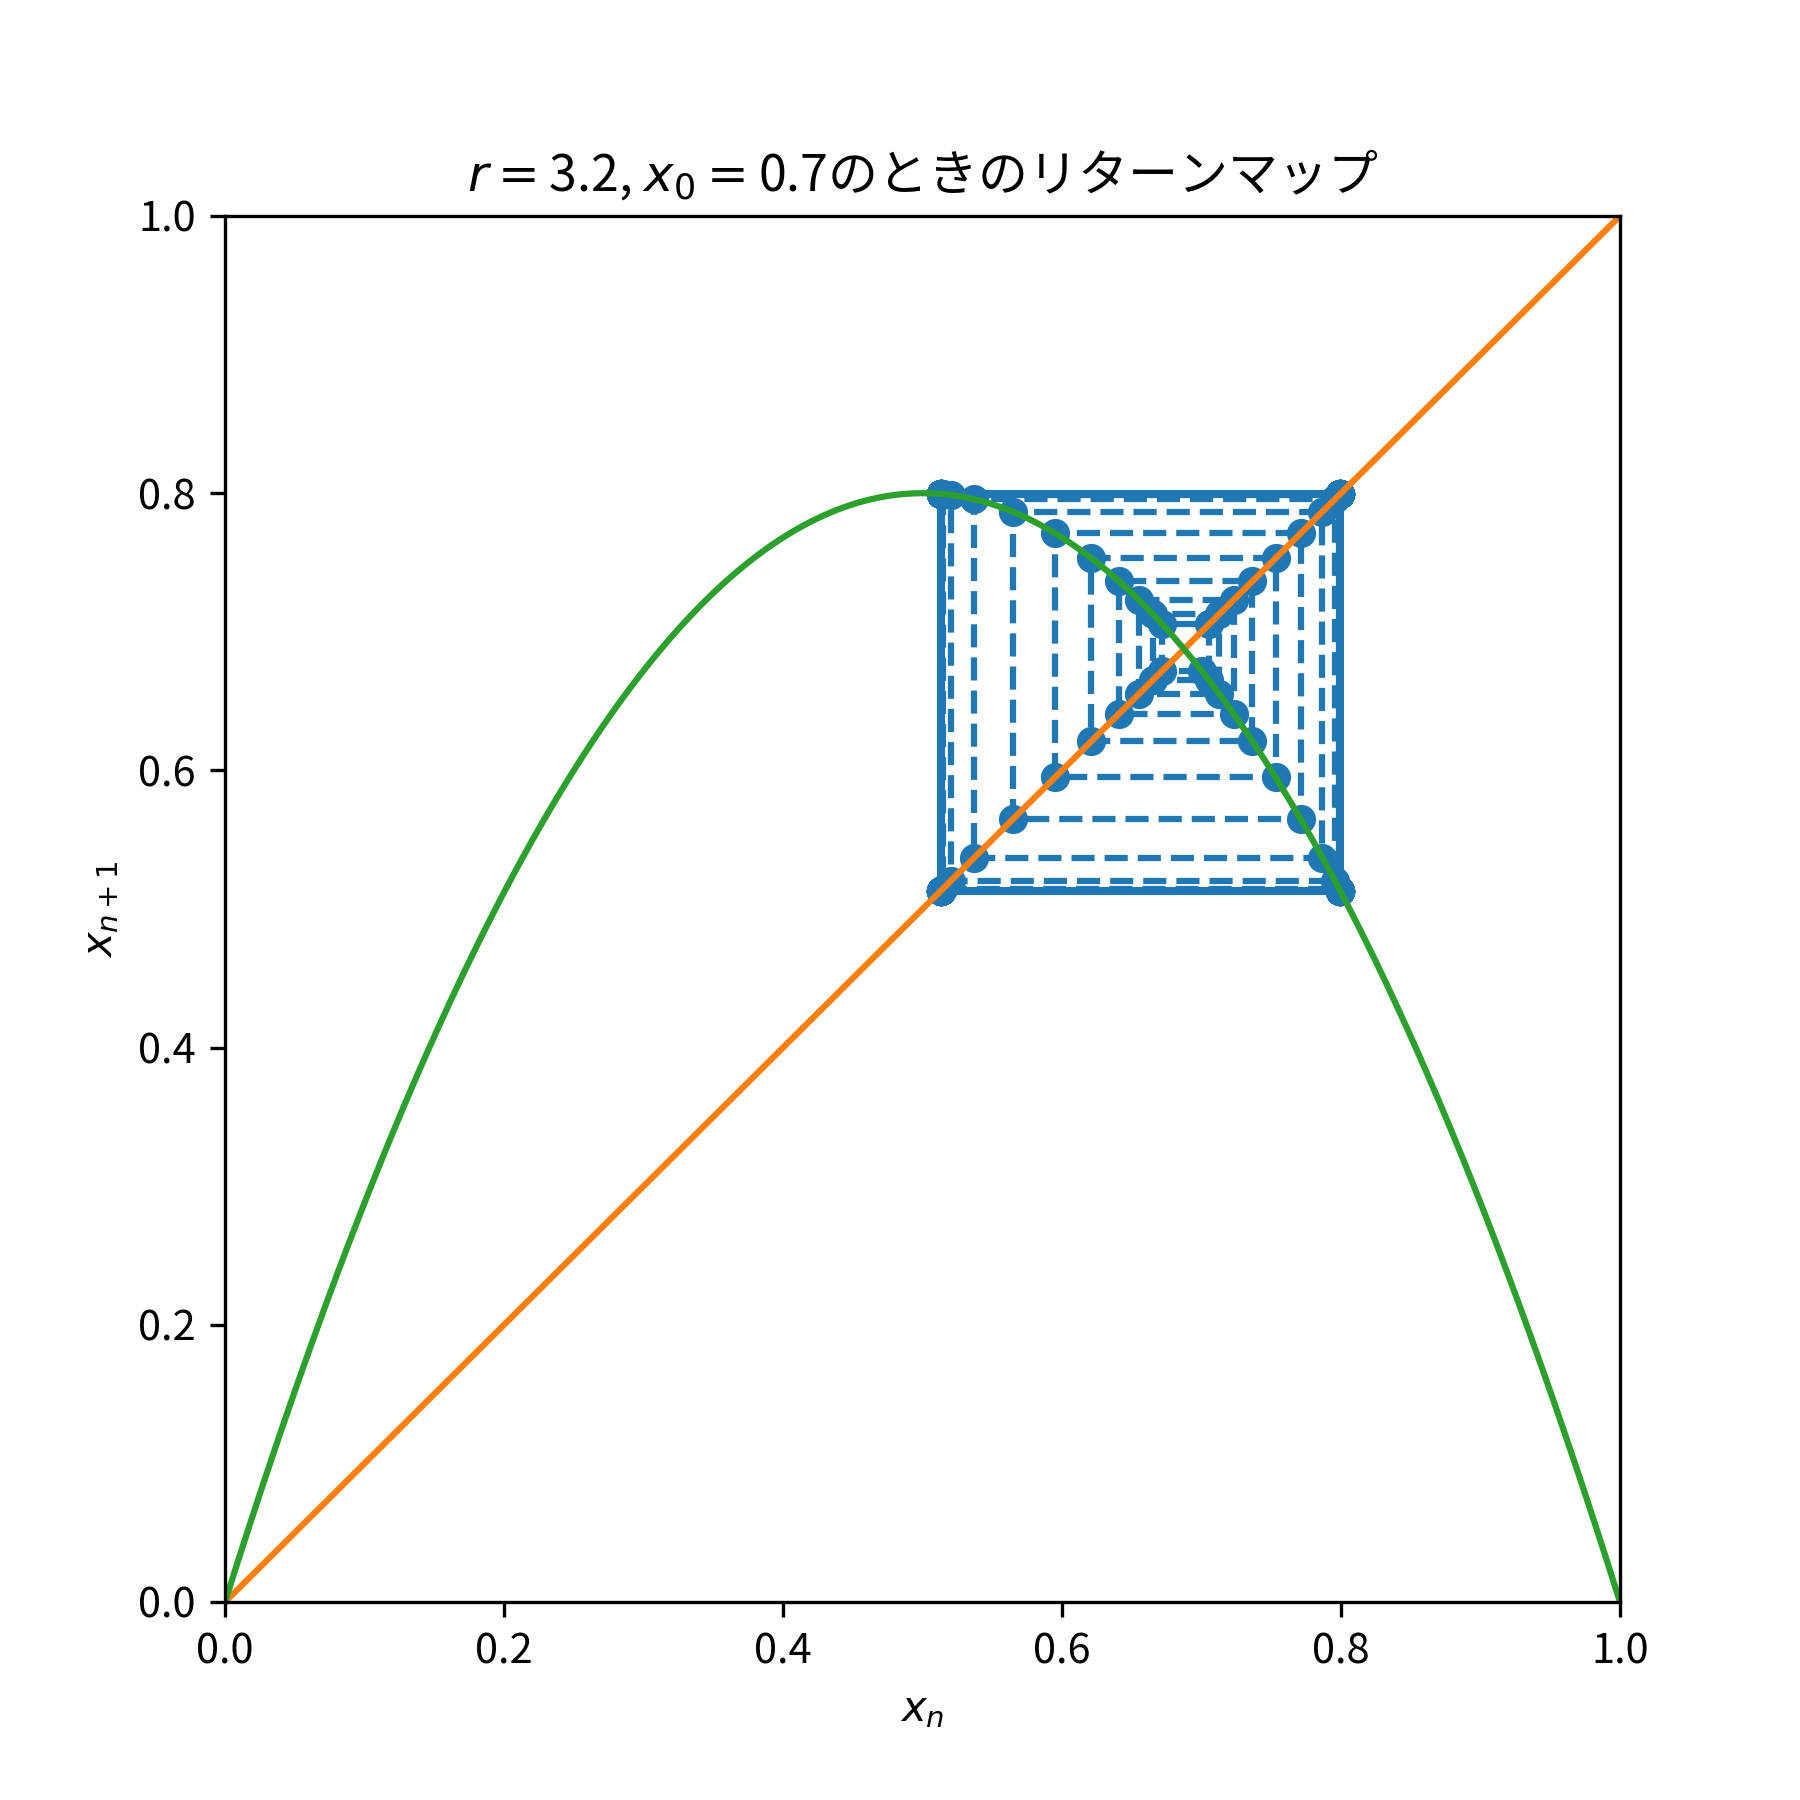
\includegraphics[keepaspectratio, scale=0.3]{images/Problem1/ctest2_3_2.png}
    \end{minipage} &
    \begin{minipage}[t]{0.45\hsize}
      \centering
      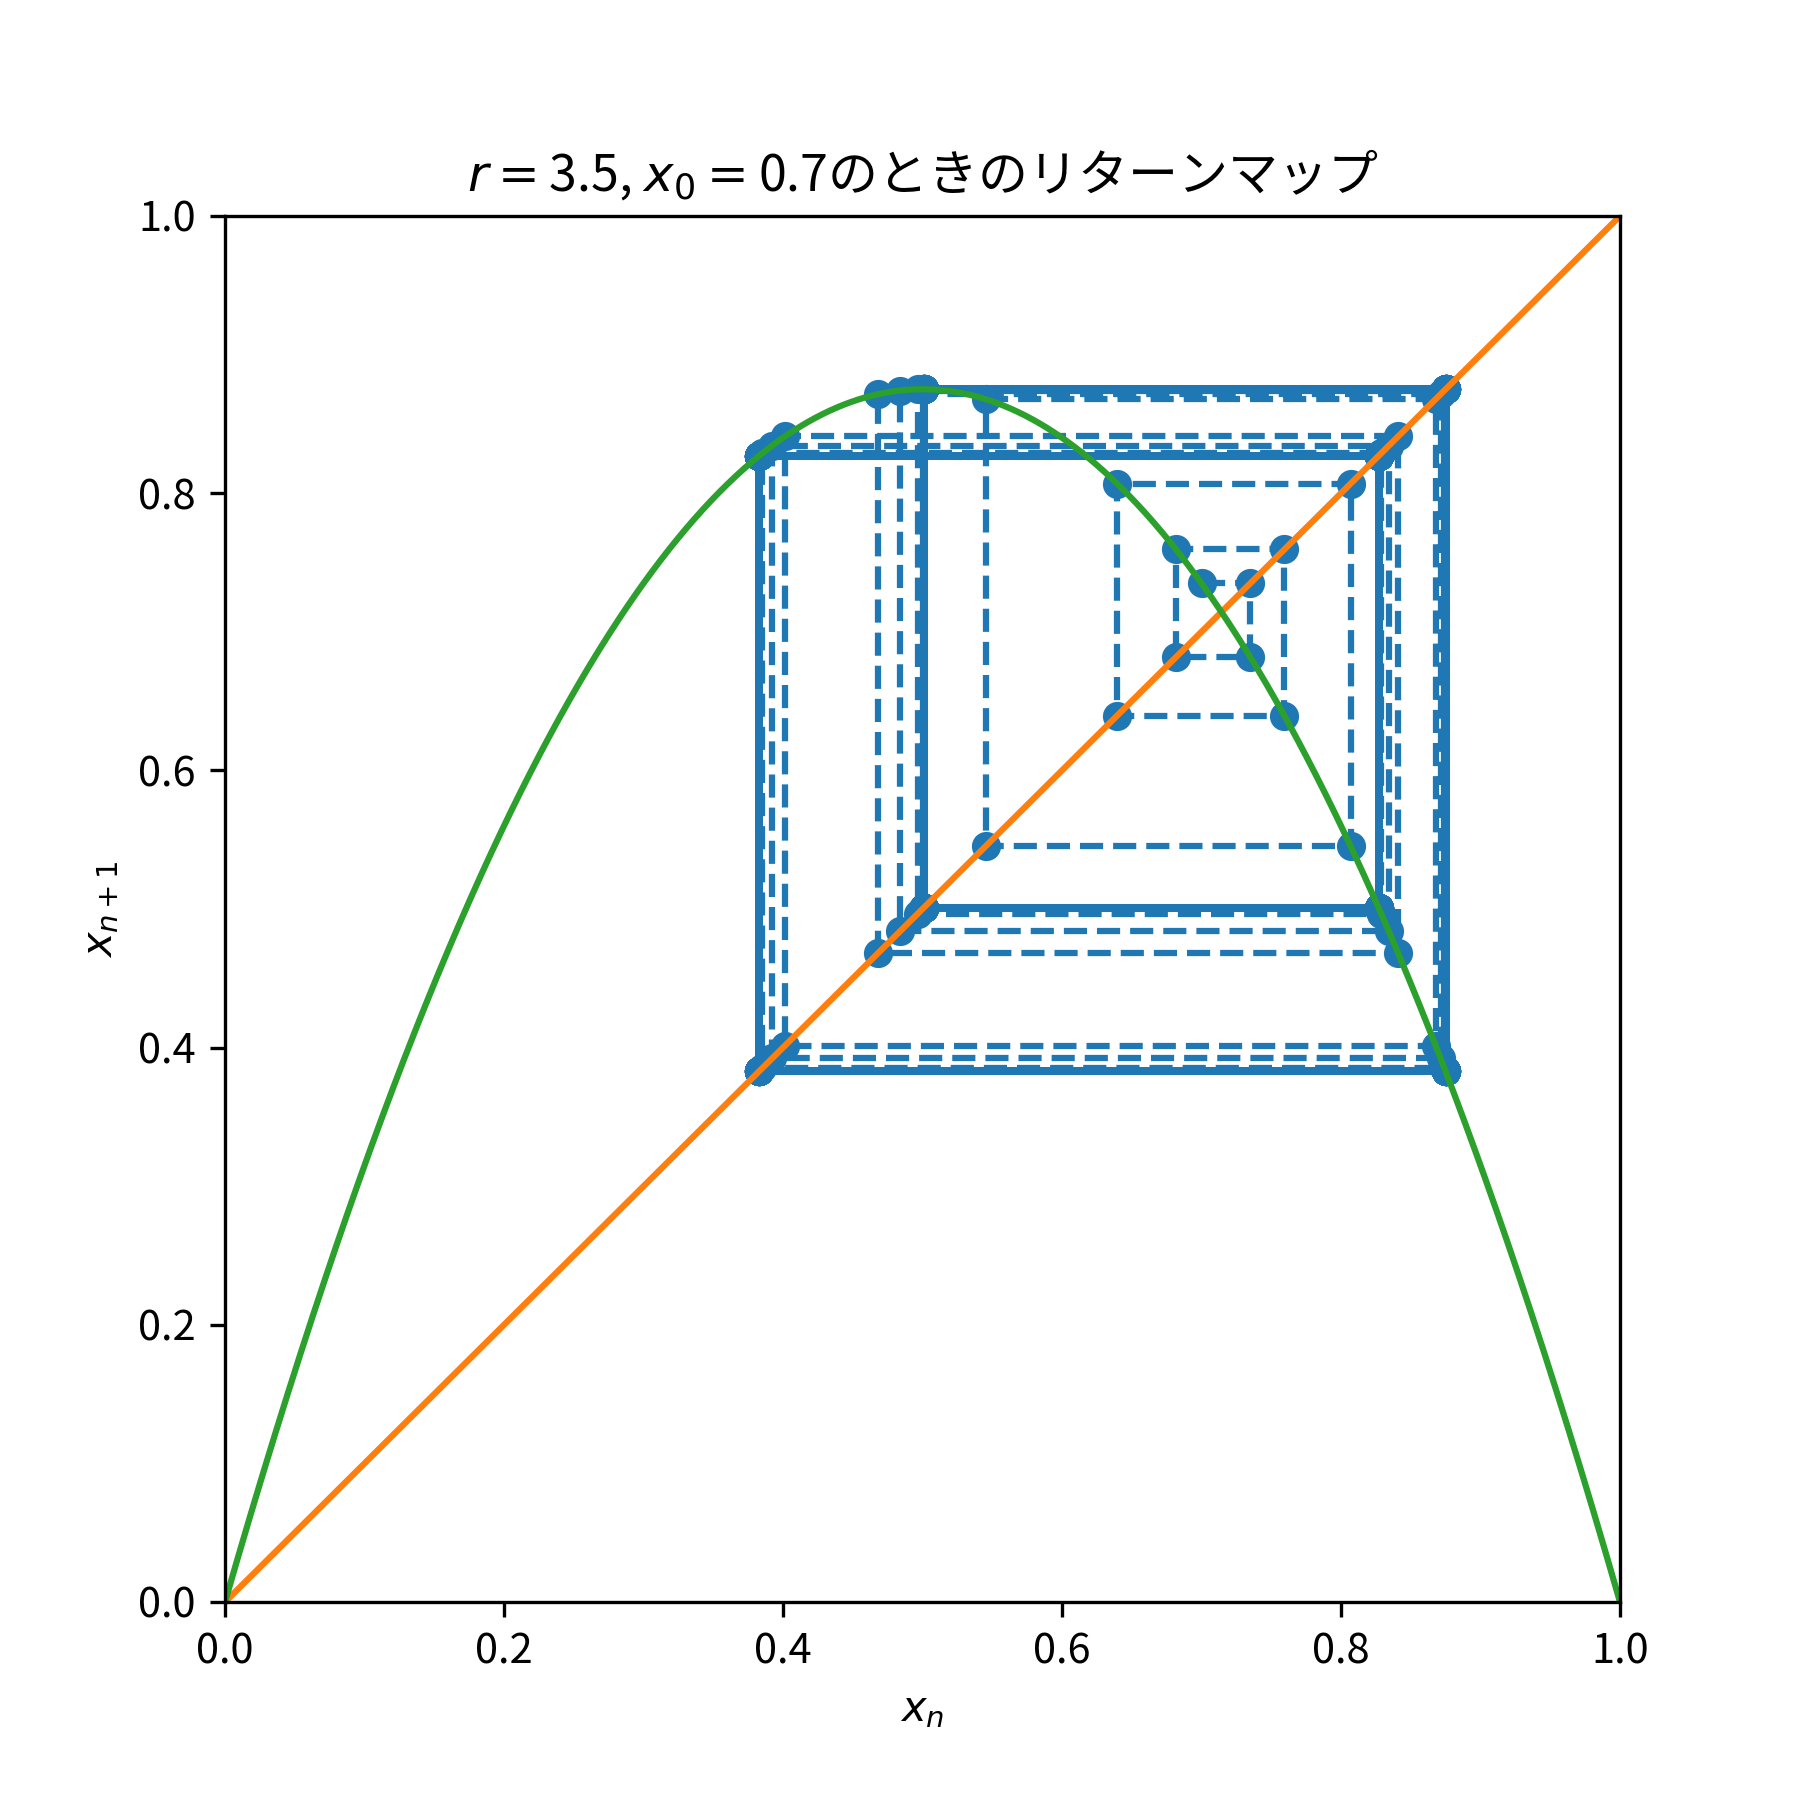
\includegraphics[keepaspectratio, scale=0.3]{images/Problem1/ctest2_4_2.png}
    \end{minipage} \\

    \begin{minipage}[t]{0.45\hsize}
      \centering
      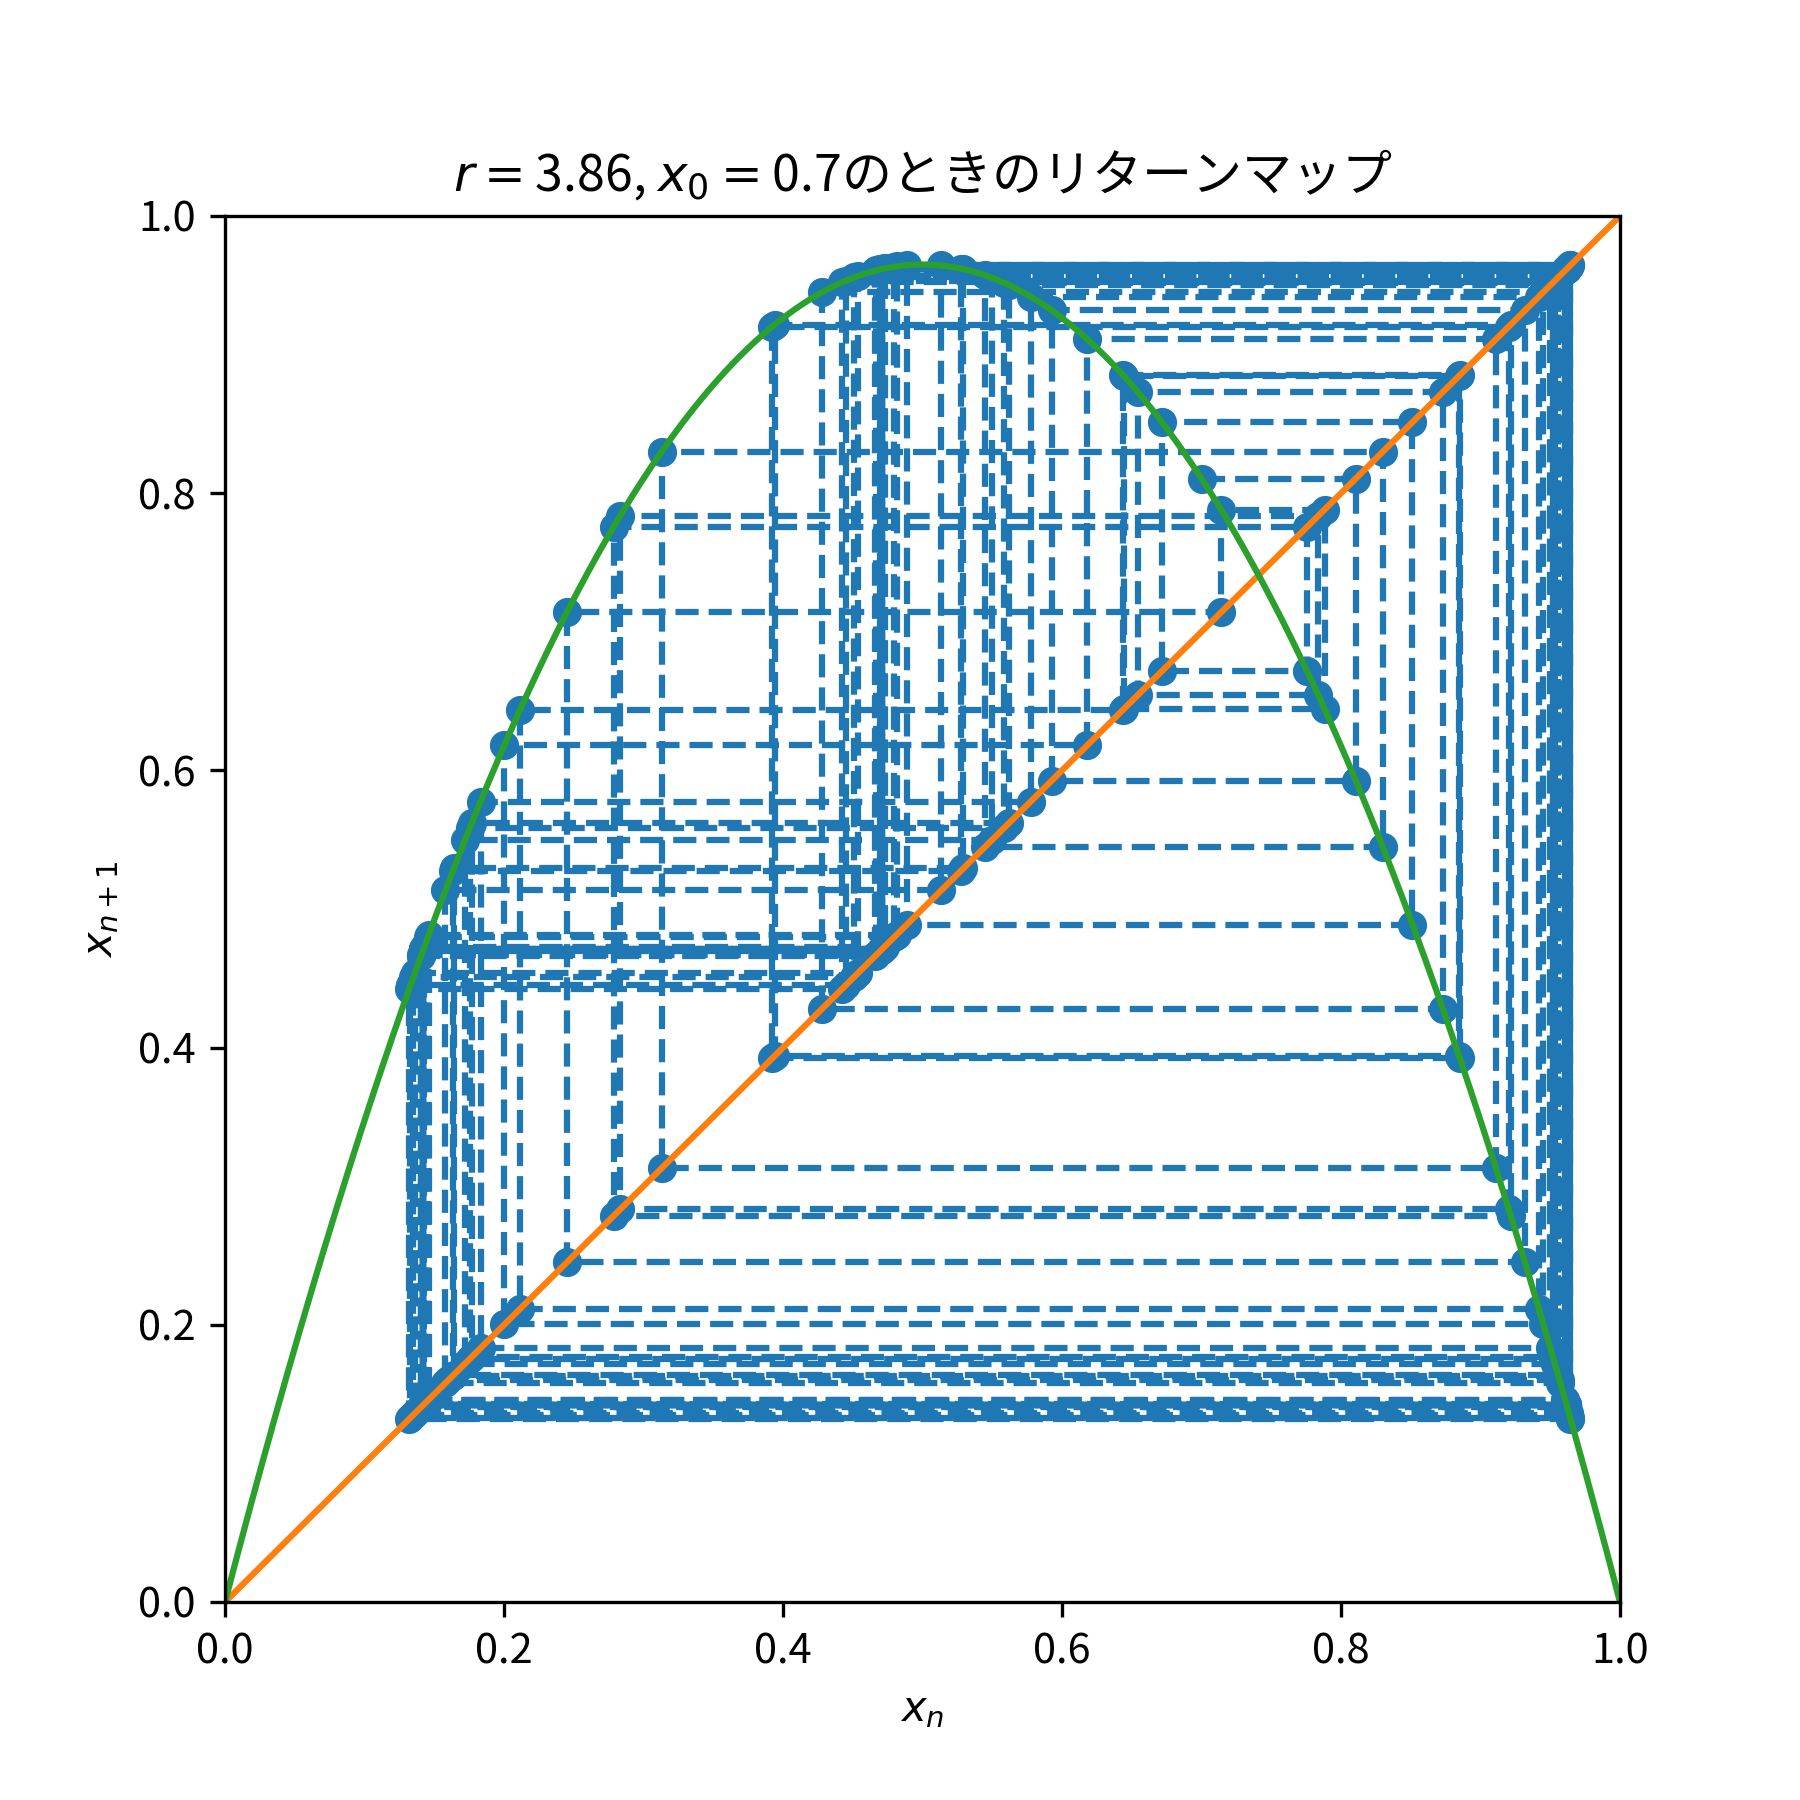
\includegraphics[keepaspectratio, scale=0.3]{images/Problem1/ctest2_5_2.png}
    \end{minipage} &
    \begin{minipage}[t]{0.45\hsize}
      \centering
      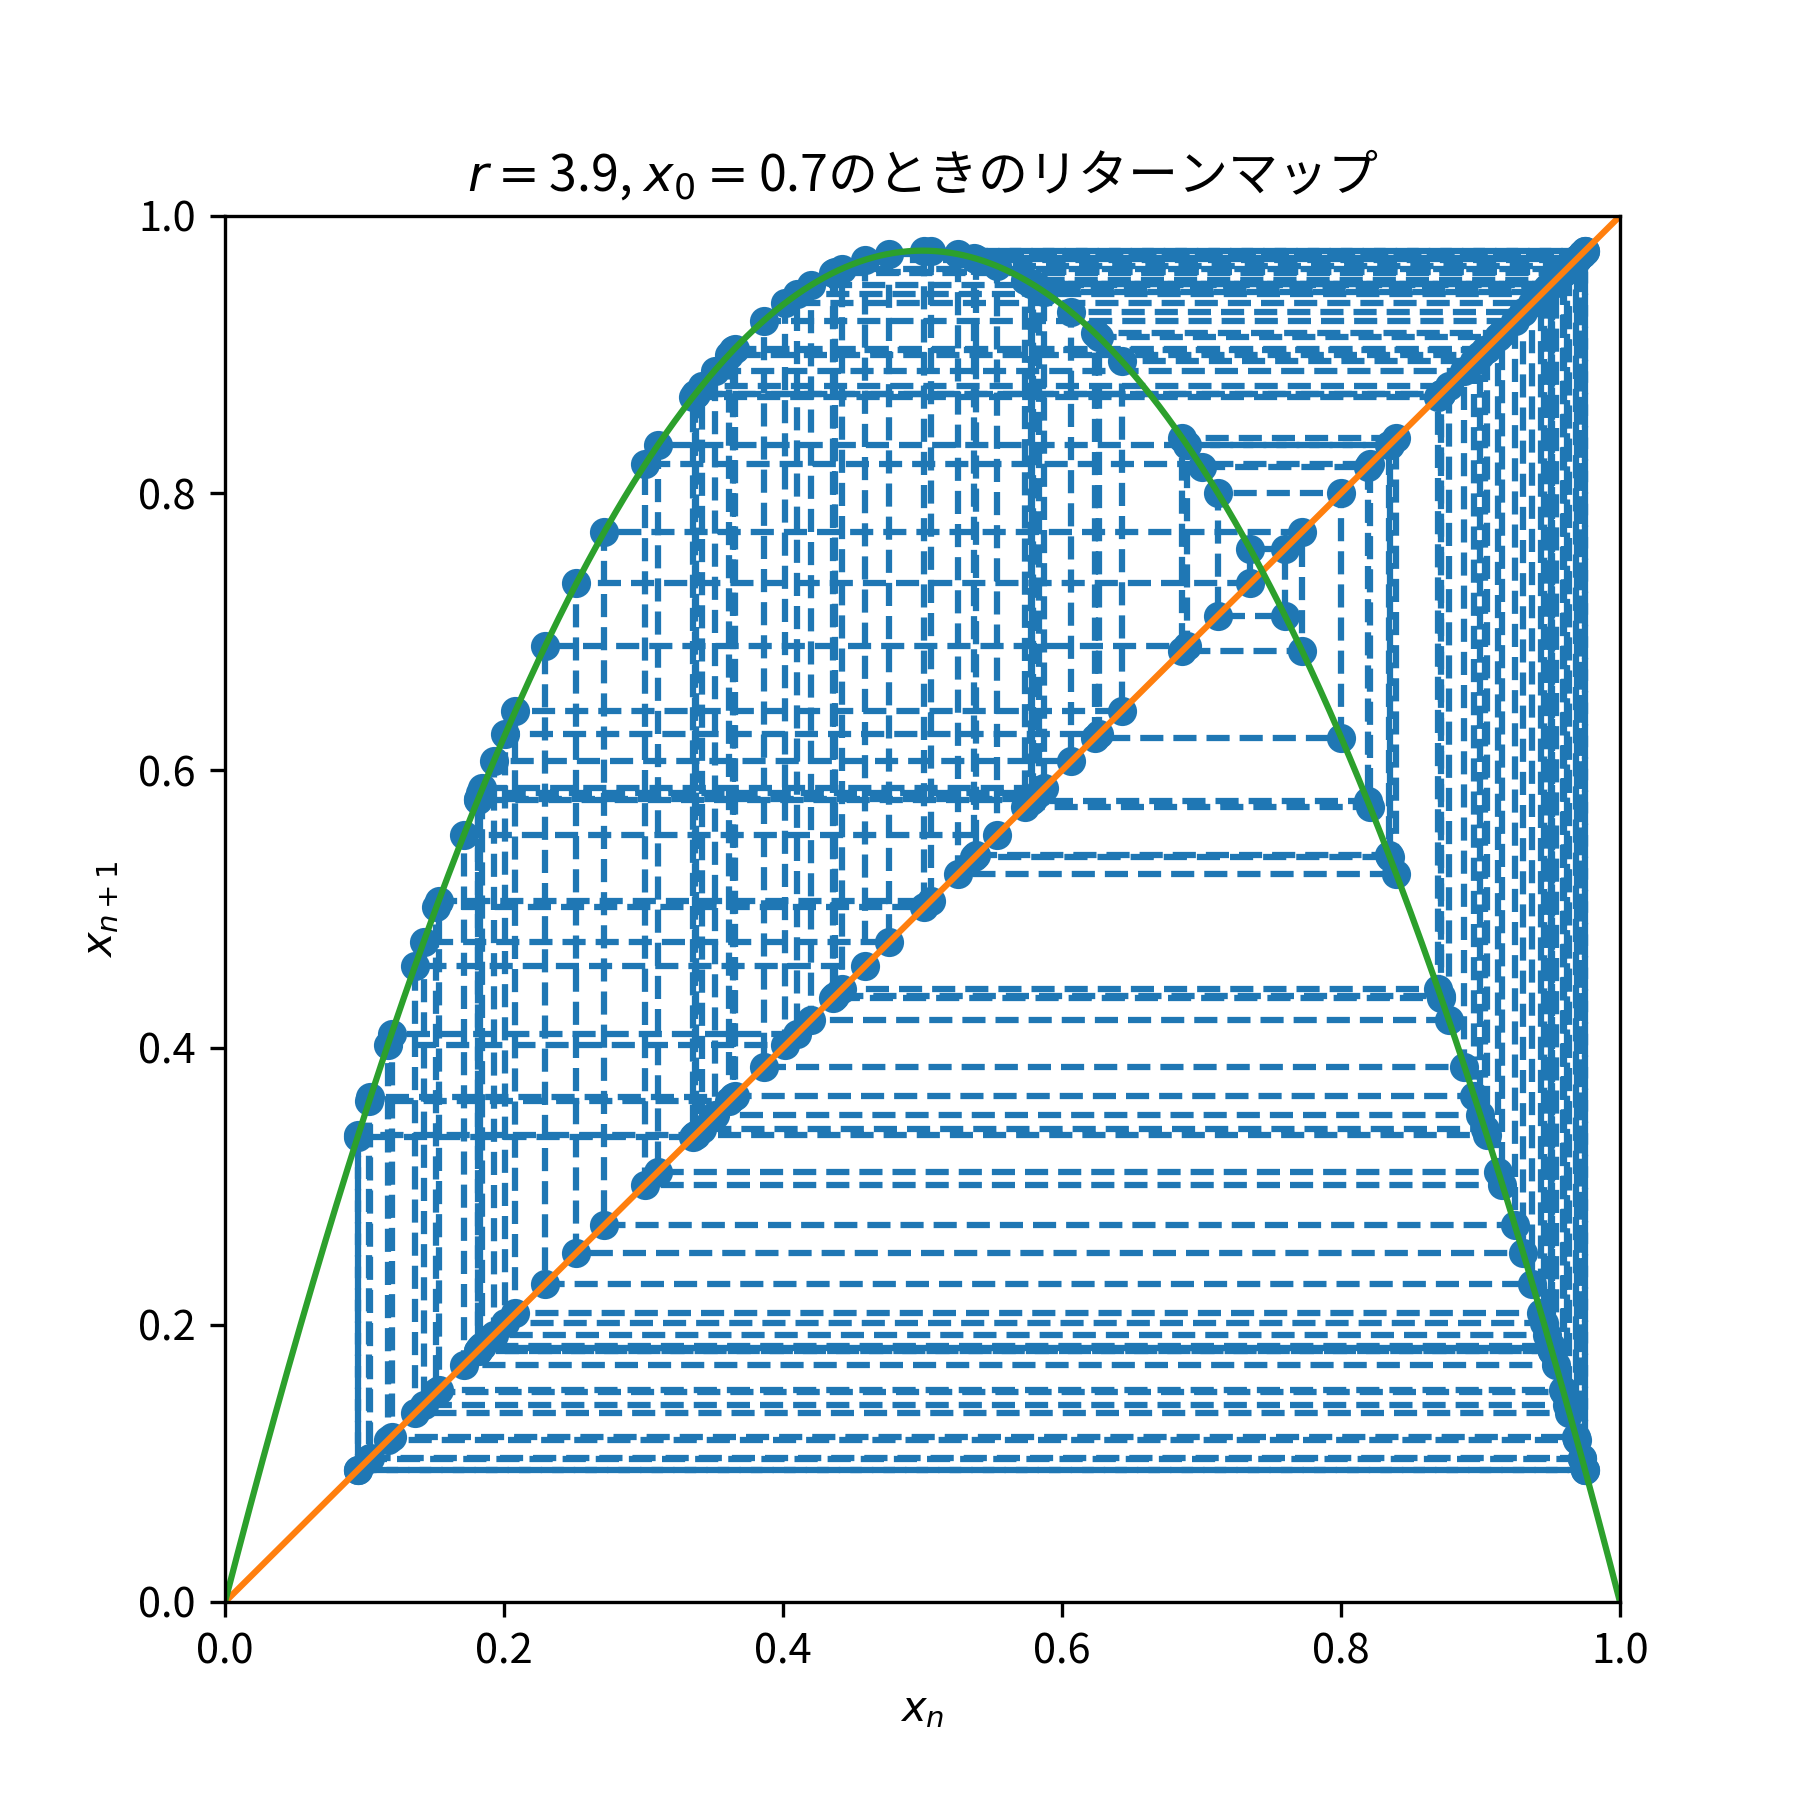
\includegraphics[keepaspectratio, scale=0.3]{images/Problem1/ctest2_6_2.png}
    \end{minipage}
  \end{tabular}
\end{figure}

結果:\\
リターンマップは、オレンジの線分が $x_{n+1} = x_n$ を示していて緑の線分が$x_{n+1} = r(1 −x_n)x_n$ を示している。時系列グラフをもとにリターンマップが描かれていくため、特徴としては似ている部分が多い。 $r = 1.50, 2.60$ のときは値が収束していき、その他では値が反復したり一切反復しないものなどがあり値は収束しない。\\\\

考察:\\
課題1, 課題2の結果から $x_{n+1} = r(1 −x_n)x_n$ と $x_{n+1} = x_n$、 $x_0$ の位置関係によって値が収束するかどうか、またカオスの状態かそうでないかが判断できるであろうと考察した。
\subsection{ソースコード}
\begin{lstlisting}[caption=week1.py]
  from matplotlib import pyplot as plt
  import numpy as np
  
  
  class Task1():
      def __init__(self, r, s) -> None:
          self.x = 0.7
          self.r = r
          self.s = s
          self.xn = np.linspace(0, 1, 1000)
          self.fig = plt.figure(figsize=(12, 6))
          self.filepath = 'Week1/images/'
  
      def logistic(self) -> list:
          "ロジスティック回帰の計算"
          calc_x = self.x
          x_array = [calc_x]
          for n in range(1, 102):
              calc_x = self.r * (1 - calc_x) * calc_x
              x_array.append(calc_x)
          return x_array
  
      def plot_time_graph(self) -> None:
          "時系列グラフの描画"
          ax2 = self.fig.add_subplot(1, 2, 2)
          n = list(range(0, 101))
          ax2.plot(n, self.logistic()[:101])
          ax2.set_title("$r = $" + str(self.r) + ", $x_0 = $" +
                        str(self.x) + 'のときの時系列グラフ')
          ax2.set_xlim(0, 100)
          ax2.set_ylim(0, 1)
          ax2.set_xlabel("$n$")
          ax2.set_ylabel("$x_n$")
  
      def plot_time_graph_only(self) -> None:
          "時系列グラフの描画のみ"
          self.fig = plt.figure(figsize=(6, 6))
          n = list(range(0, 101))
          plt.plot(n, self.logistic()[:101])
          plt.title("$r = $" + str(self.r) + ", $x_0 = $" +
                    str(self.x) + 'のときの時系列グラフ')
          plt.xlim(0, 100)
          plt.ylim(0, 1)
          plt.xlabel("$n$")
          plt.ylabel("$x_n$")
          plt.savefig(self.filepath + self.s + '_1', dpi=300)
  
      def plot_return_map(self) -> None:
          "リターンマップの描画"
          ax1 = self.fig.add_subplot(1, 2, 1)
          xn_array = []
          for i in self.xn:
              xn_array.append(self.r * (1 - i) * i)
          # クモの巣図用の配列
          n = self.logistic()
          spiper_plot_x = []
          spiper_plot_y = []
          for i in range(1, len(n)):
              spiper_plot_x.append(n[i - 1])
              spiper_plot_x.append(n[i])
              spiper_plot_y.append(n[i])
              spiper_plot_y.append(n[i])
  
          ax1.plot(spiper_plot_x, spiper_plot_y, marker='o', linestyle='dashed')
          ax1.plot(self.xn, self.xn)
          ax1.plot(self.xn, xn_array)
          ax1.set_title("$r = $" + str(self.r) + ", $x_0 = $" +
                        str(self.x) + 'のときのリターンマップ')
          ax1.set_xlim(0, 1)
          ax1.set_ylim(0, 1)
          ax1.set_xlabel("$x_n$")
          ax1.set_ylabel("$x_{n+1}$")
  
      def plot_return_map_only(self) -> None:
          "リターンマップの描画のみ"
          self.fig = plt.figure(figsize=(6, 6))
          xn_array = []
          for i in self.xn:
              xn_array.append(self.r * (1 - i) * i)
          # クモの巣図用の配列
          n = self.logistic()
          spiper_plot_x = []
          spiper_plot_y = []
          for i in range(1, len(n)):
              spiper_plot_x.append(n[i - 1])
              spiper_plot_x.append(n[i])
              spiper_plot_y.append(n[i])
              spiper_plot_y.append(n[i])
  
          plt.plot(spiper_plot_x, spiper_plot_y, marker='o', linestyle='dashed')
          plt.plot(self.xn, self.xn)
          plt.plot(self.xn, xn_array)
          plt.title("$r = $" + str(self.r) + ", $x_0 = $" +
                    str(self.x) + 'のときのリターンマップ')
          plt.xlim(0, 1)
          plt.ylim(0, 1)
          plt.xlabel("$x_n$")
          plt.ylabel("$x_{n+1}$")
          plt.savefig(self.filepath + self.s + '_2', dpi=300)
  
      def do_plot(self) -> None:
          self.plot_delta_time_graph()
          self.plot_return_map()
  
      def show_graph(self) -> None:
          plt.savefig(self.filepath + self.s, dpi=300)
          # plt.show()
  
  
  r = [1.50, 2.60, 3.20, 3.50, 3.86, 3.90]
  for i in range(len(r)):
      demo = Task1(r[i], 'ctest2_{}'.format(i + 1))
      demo.do_plot()
      demo.show_graph()
  
  for i in range(len(r)):
      for_report = Task1(r[i], 'ctest2_{}'.format(i + 1))
      for_report.plot_time_graph_only()
      for_report.plot_return_map_only()
  
\end{lstlisting}
\section{レポート課題2}
\subsection{課題1}
ジスティク写像で$r = 1.50, r = 2.60, r = 3.20, r = 3.50, r = 3.86, r = 3.90$として、初期値$x_0$を$0$から$1$まで$0.001$きざみで変化させたときの、$x_{200}$の値がどうなっているかグラフ化せよ。また、$x_n$が$150 < n < 200$の場合もグラフ化せよ。出力形式は授業資料を参照すること。\par
画像:
\begin{figure}[h]
  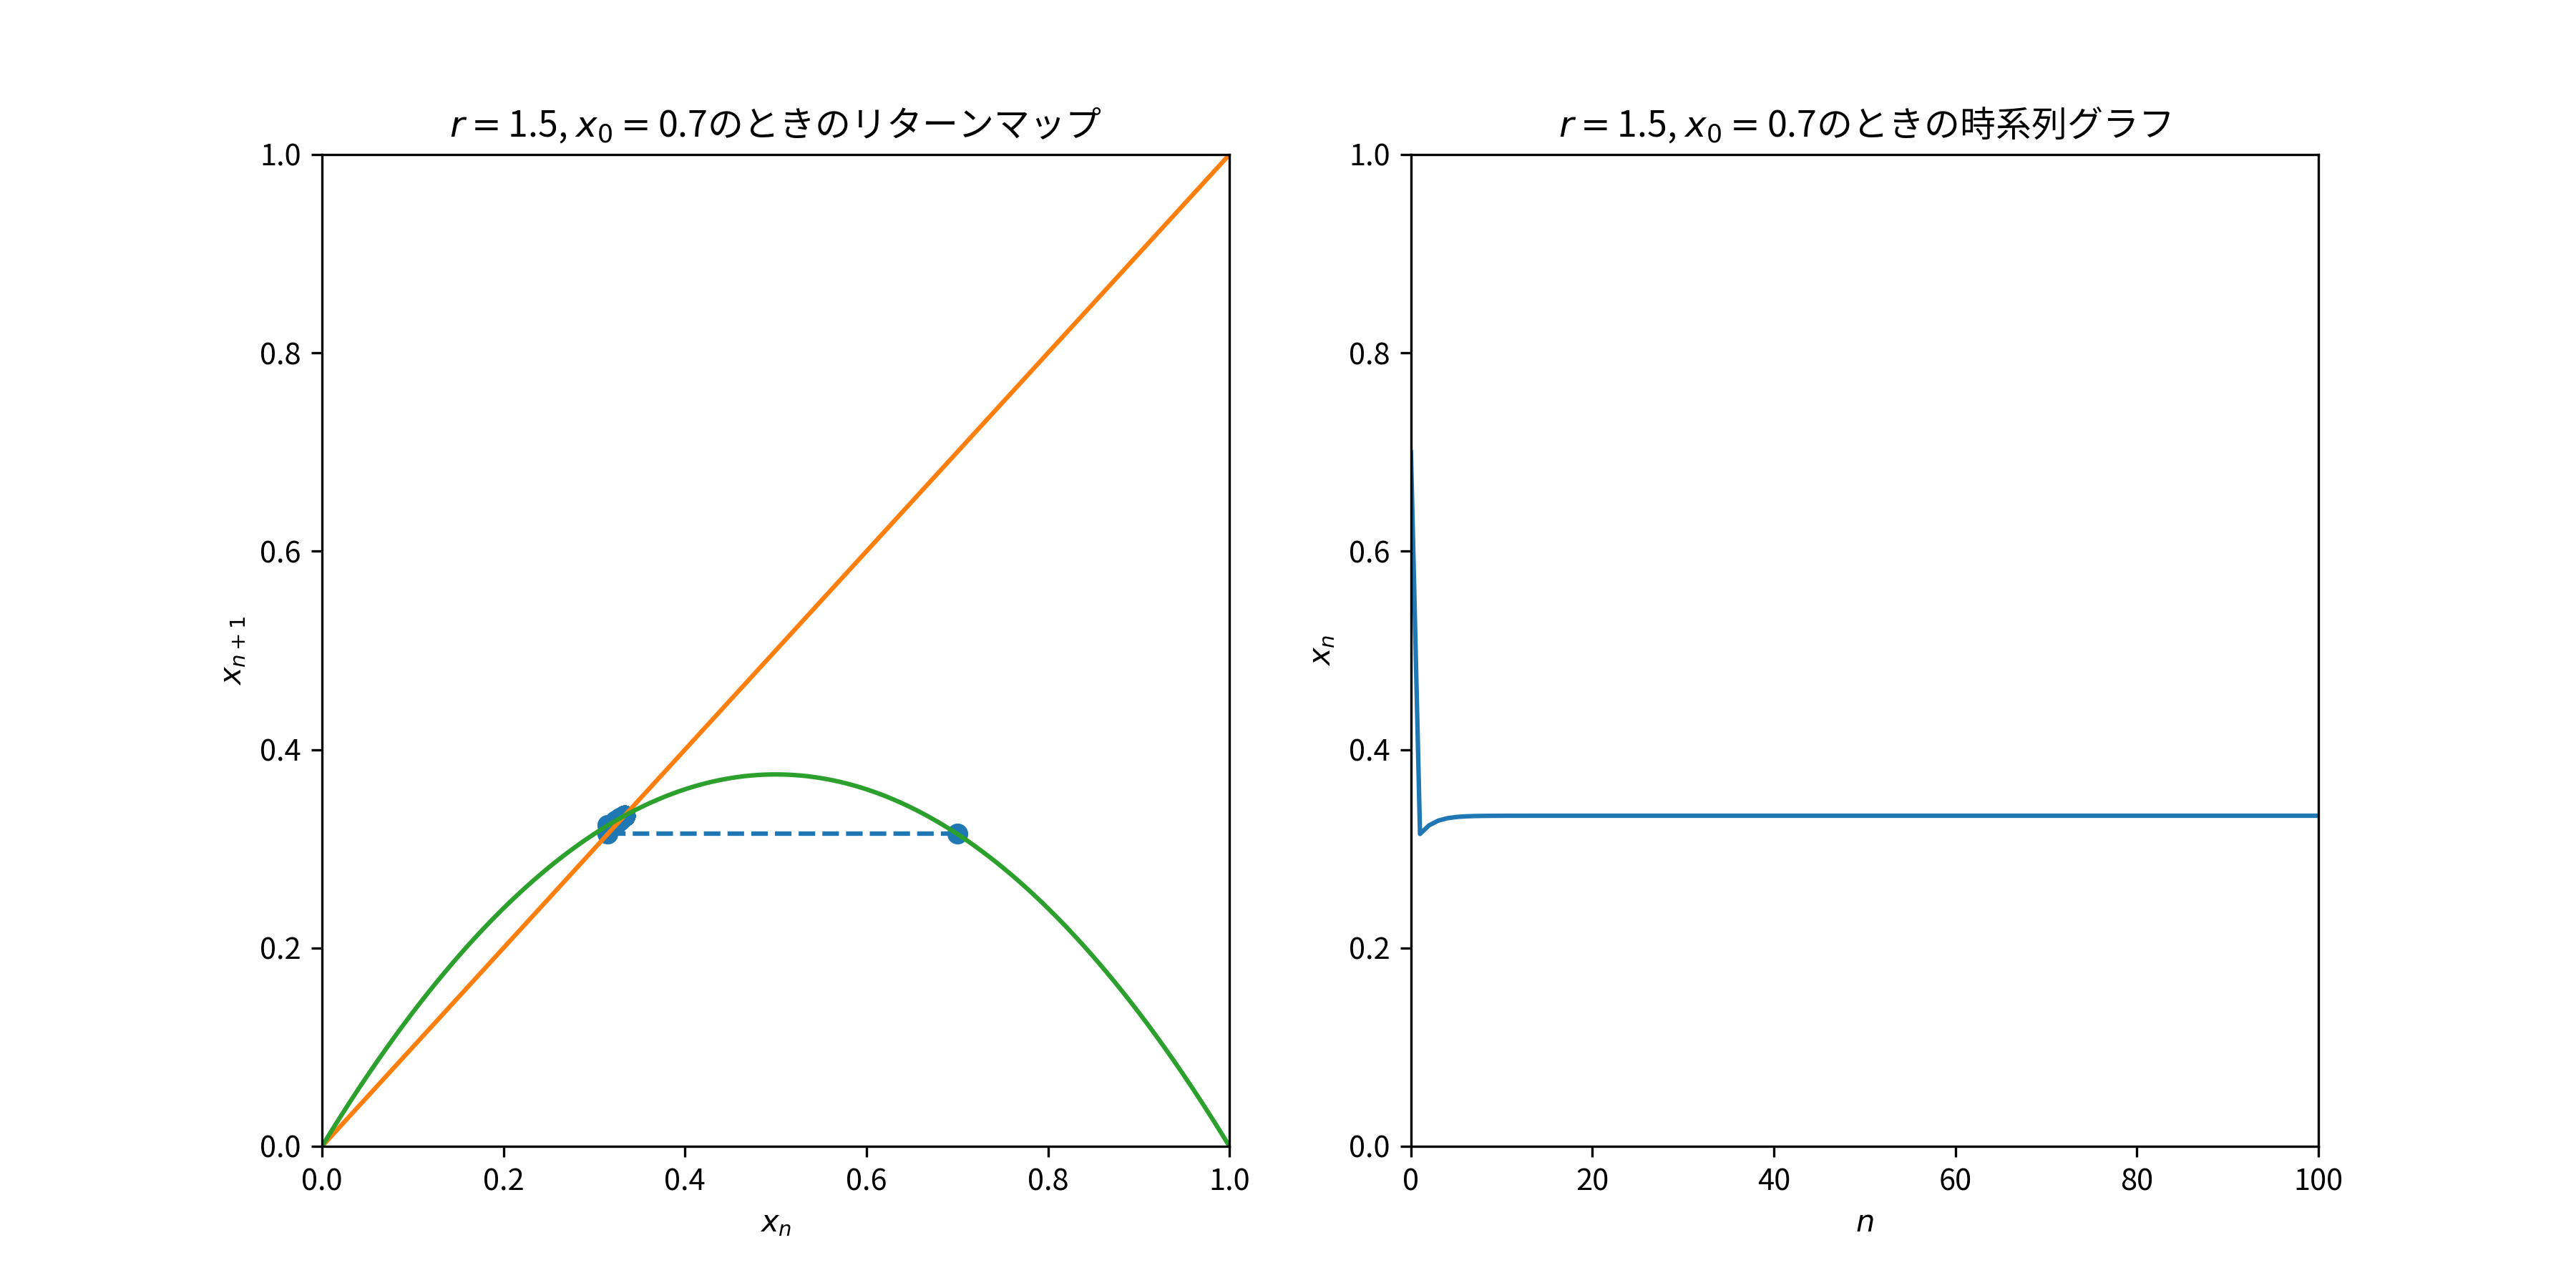
\includegraphics[width=15cm]{images/ctest2_1.png}
\end{figure}

解説:\par
この図は左にリターンマップ、右に時系列グラフをプロットした図をレポートの

\subsection{課題2}
課題1 で得られた結果から初期値鋭敏性を説明せよ。
\section{レポート課題3}
\subsection{課題1}
ロジスティク写像の初期変動の影響がないリターンマップを描くためのプログラムを作成し、個体数変動のリターンマップを表示せよ。このとき $r$ は、$r = 1.50, r = 2.60, r = 3.20, r = 3.50, r = 3.86, r = 3.90$ のとし、初期値$x_0$はランダムに与えなさい。グラフは、授業資料を参考として、 $x_{n+1} = r(1 − x_n)x_n、x_{n+1} = x_n$ も同時に描画し、縦軸と横軸は $0~1$ の範囲で出力すること。\\
画像:\\
\begin{figure}[htbp]
  \begin{tabular}{cc}
    \begin{minipage}[t]{0.45\hsize}
      \centering
      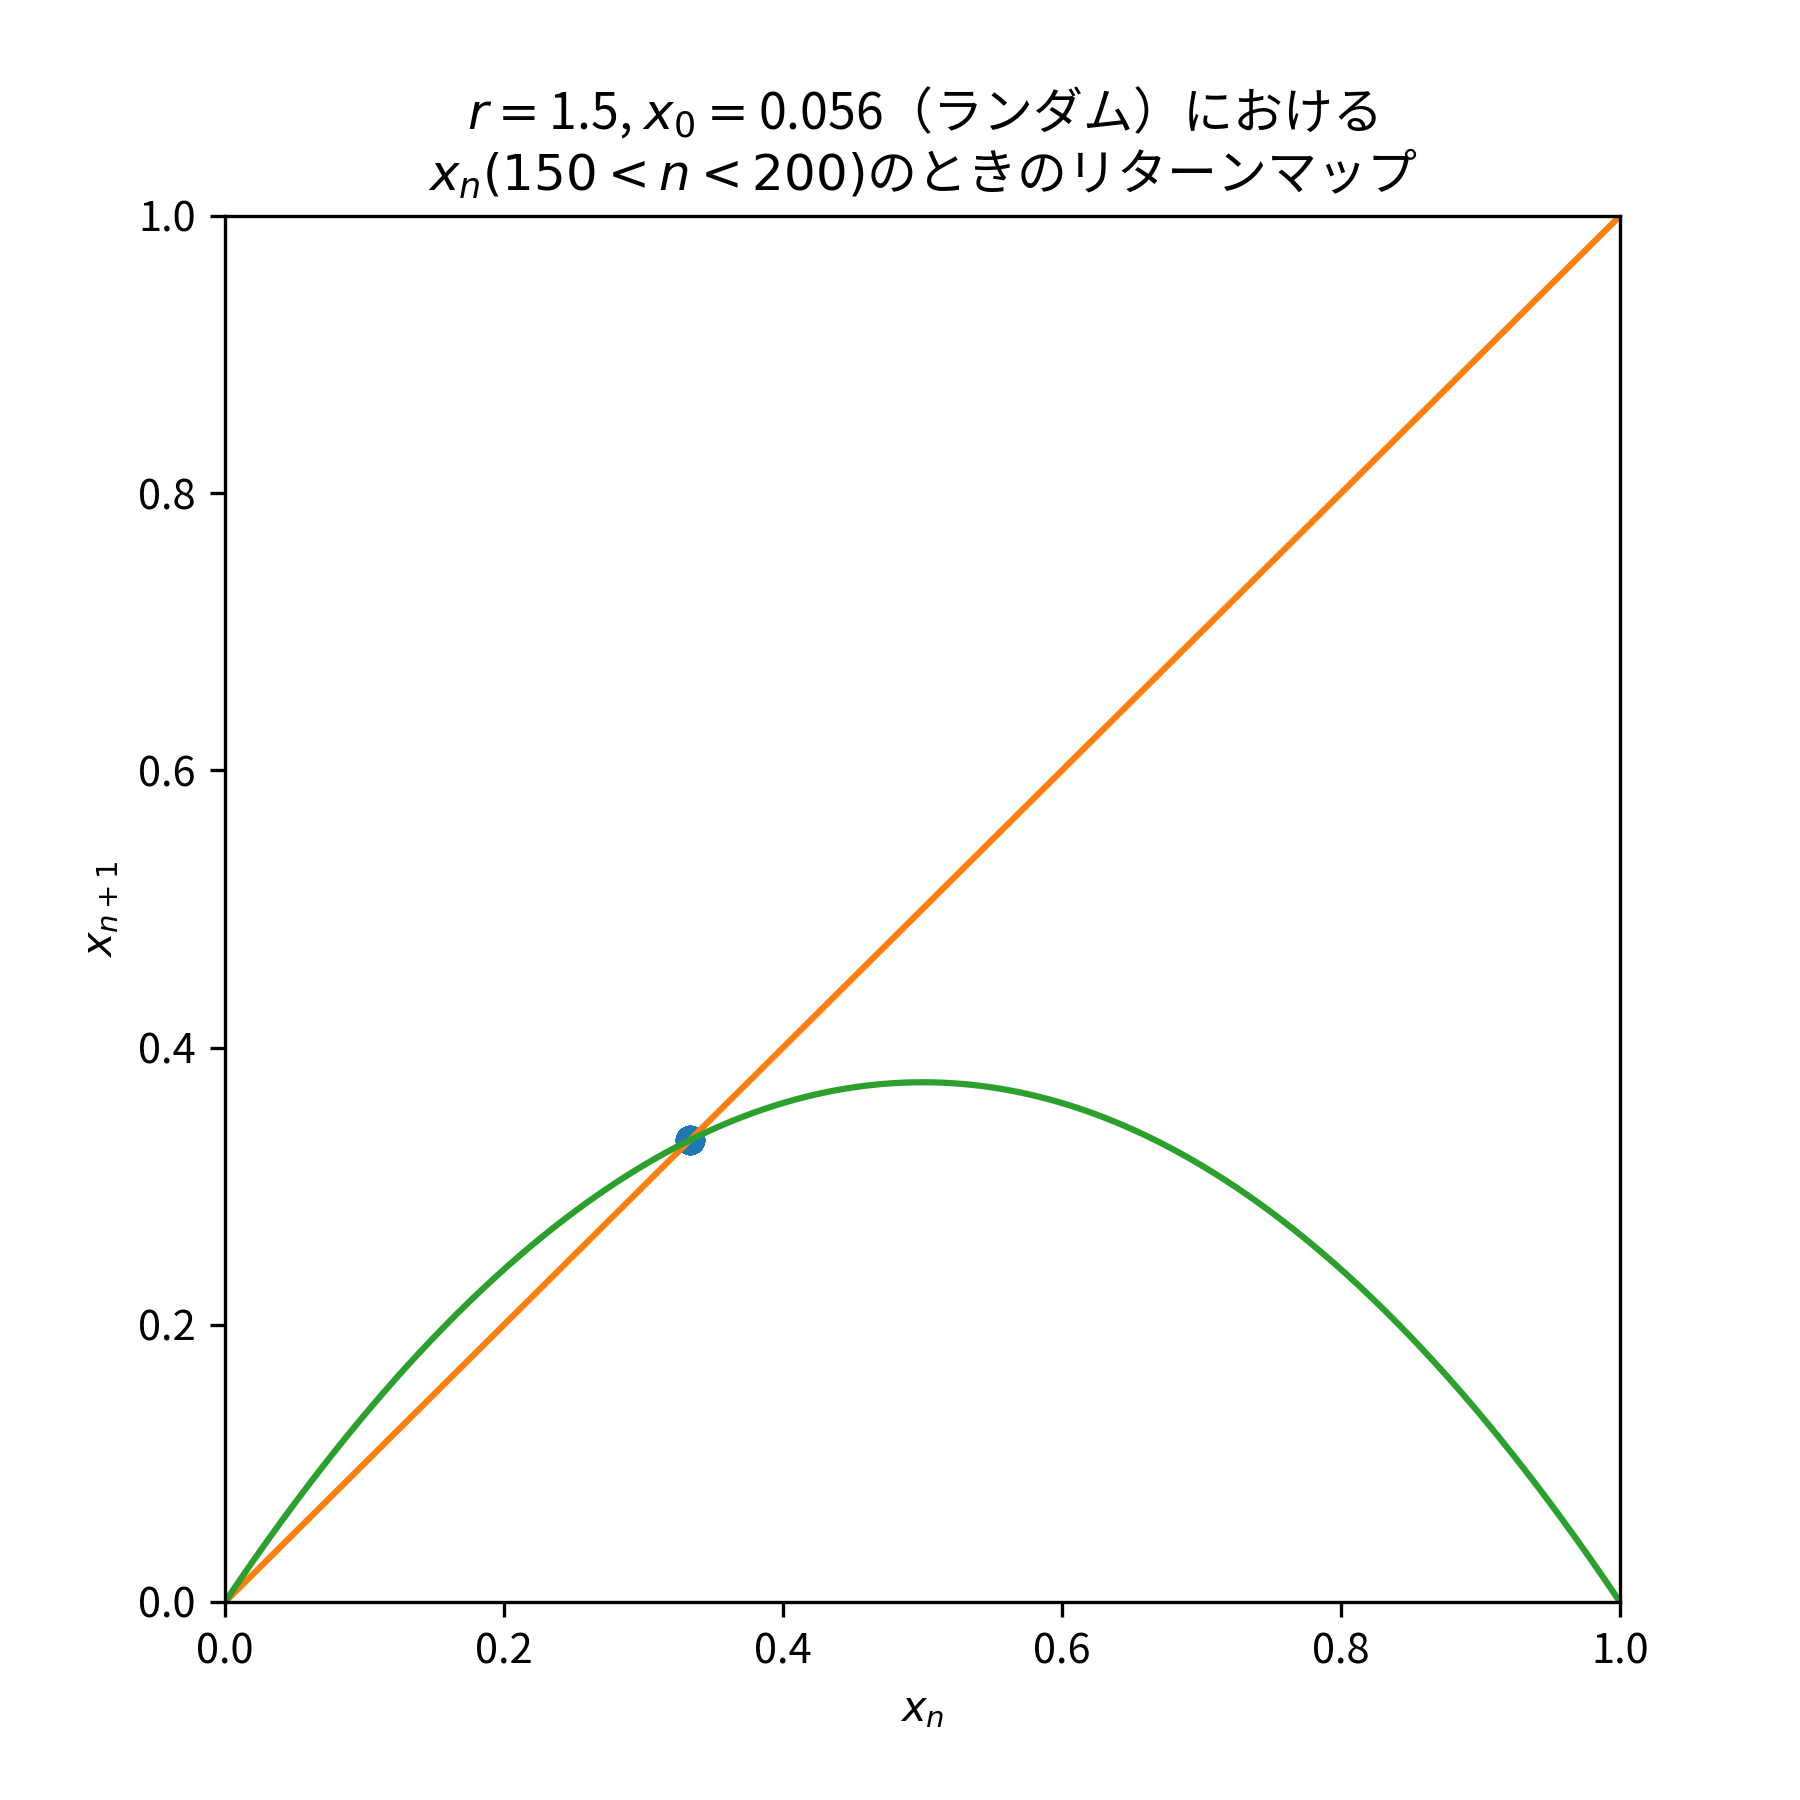
\includegraphics[keepaspectratio, scale=0.3]{images/Problem3/report4_1.png}
    \end{minipage} &
    \begin{minipage}[t]{0.45\hsize}
      \centering
      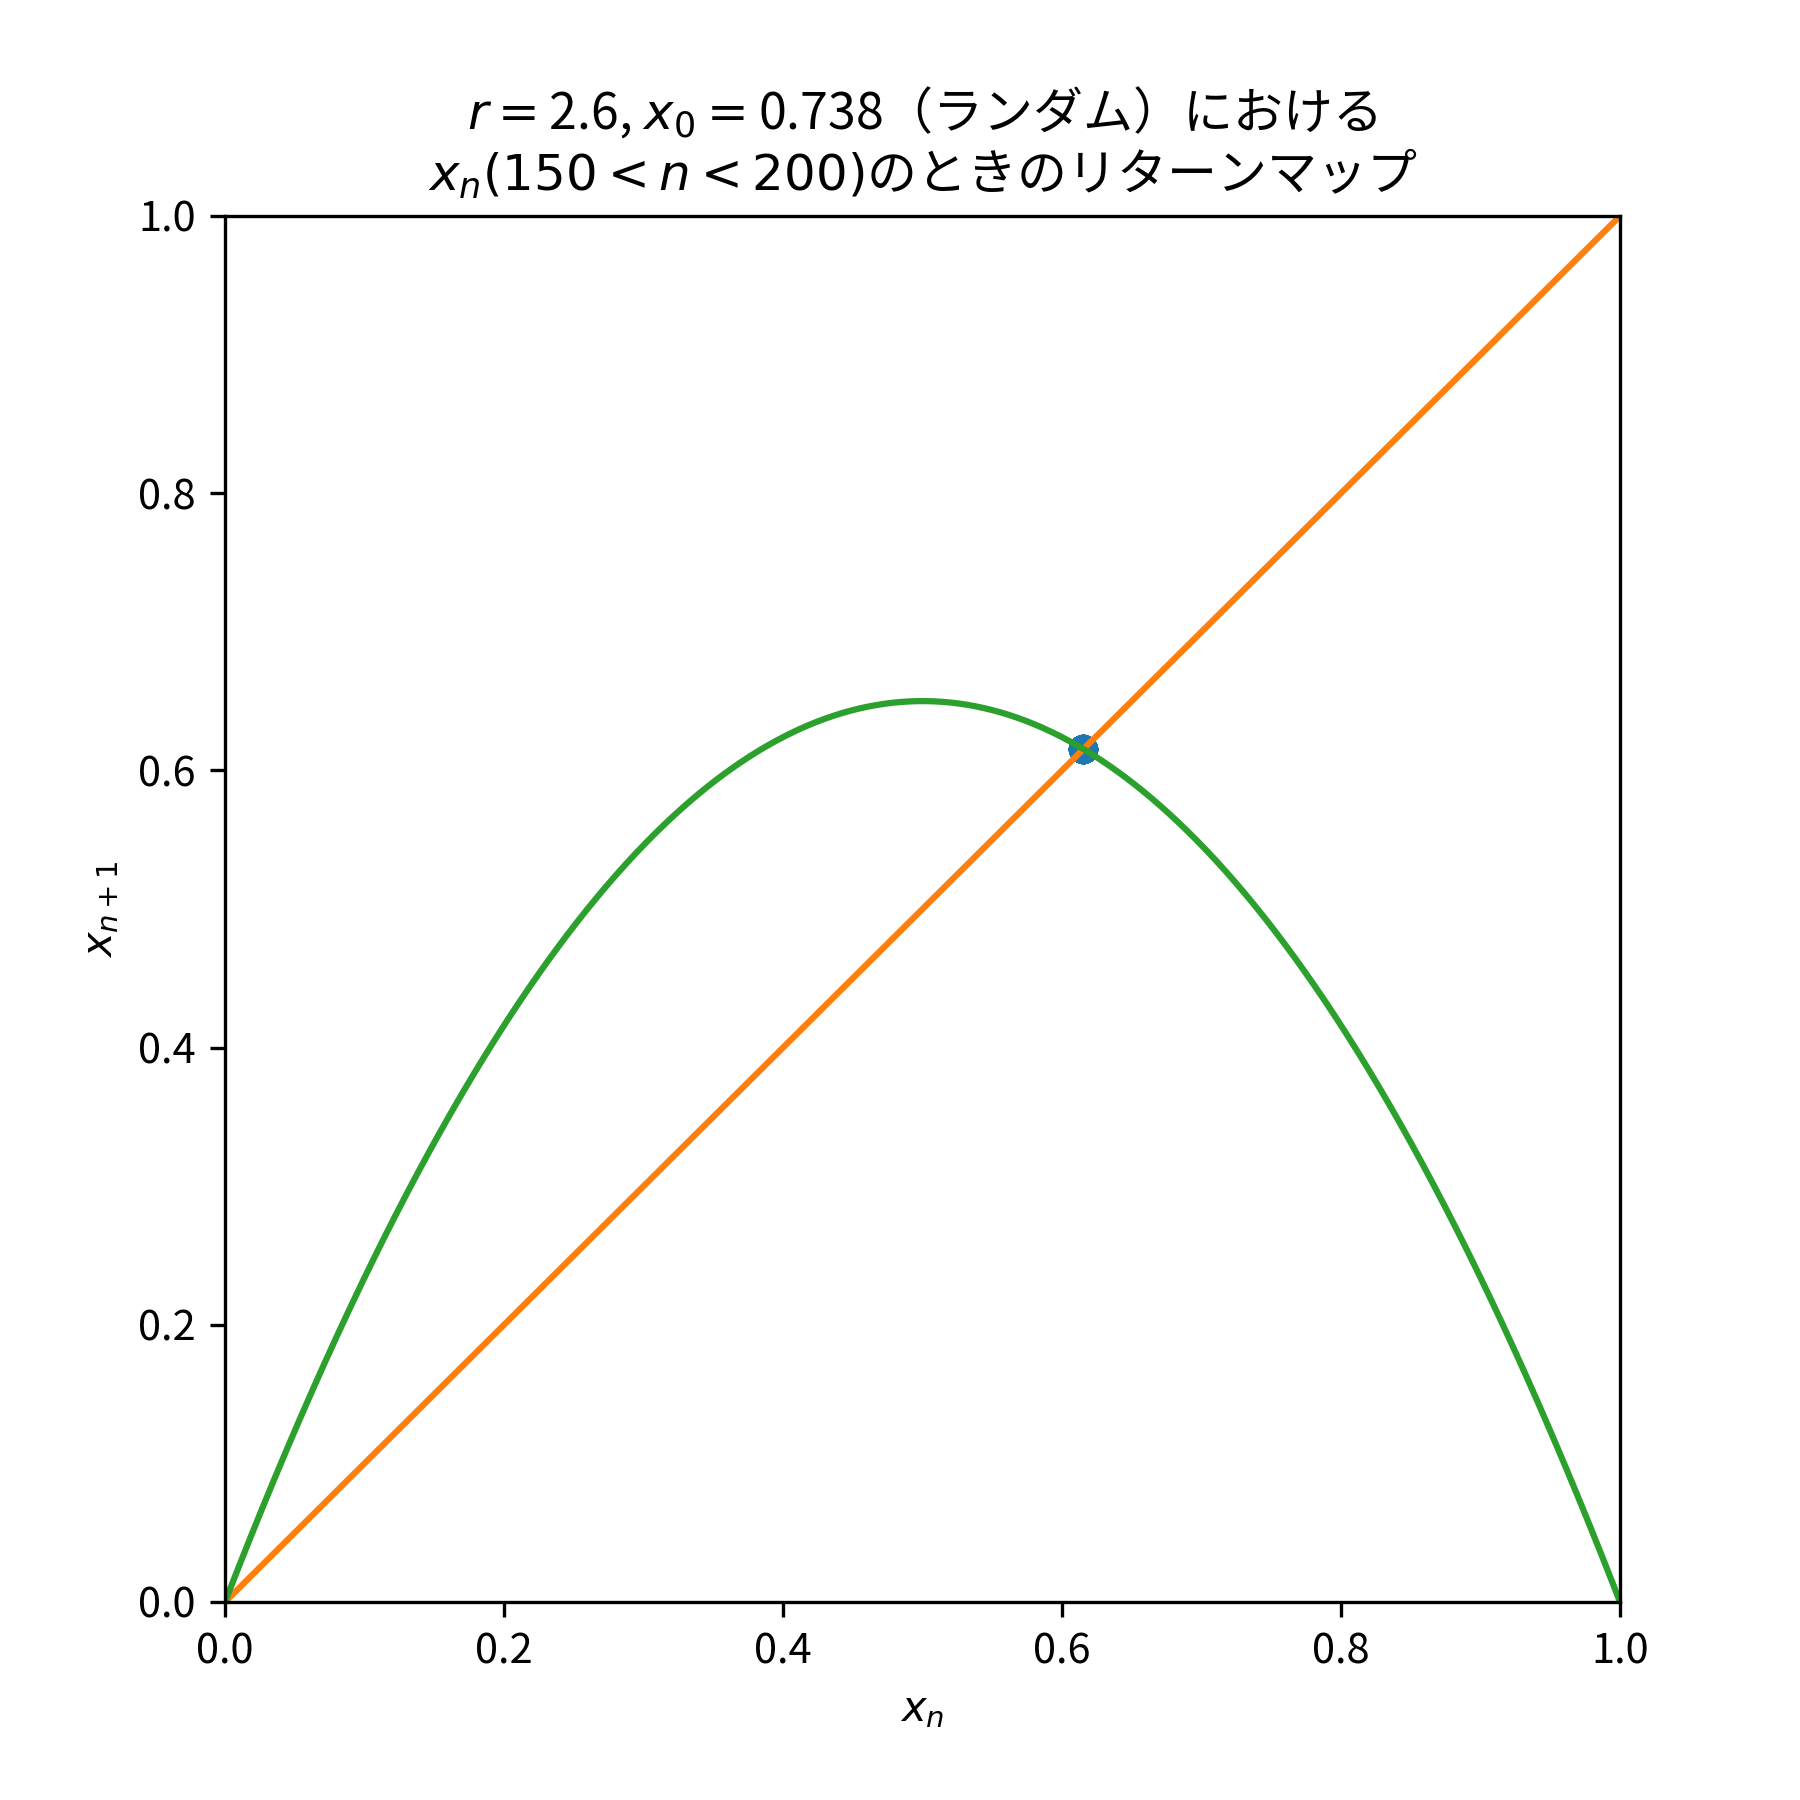
\includegraphics[keepaspectratio, scale=0.3]{images/Problem3/report4_2.png}
    \end{minipage} \\

    \begin{minipage}[t]{0.45\hsize}
      \centering
      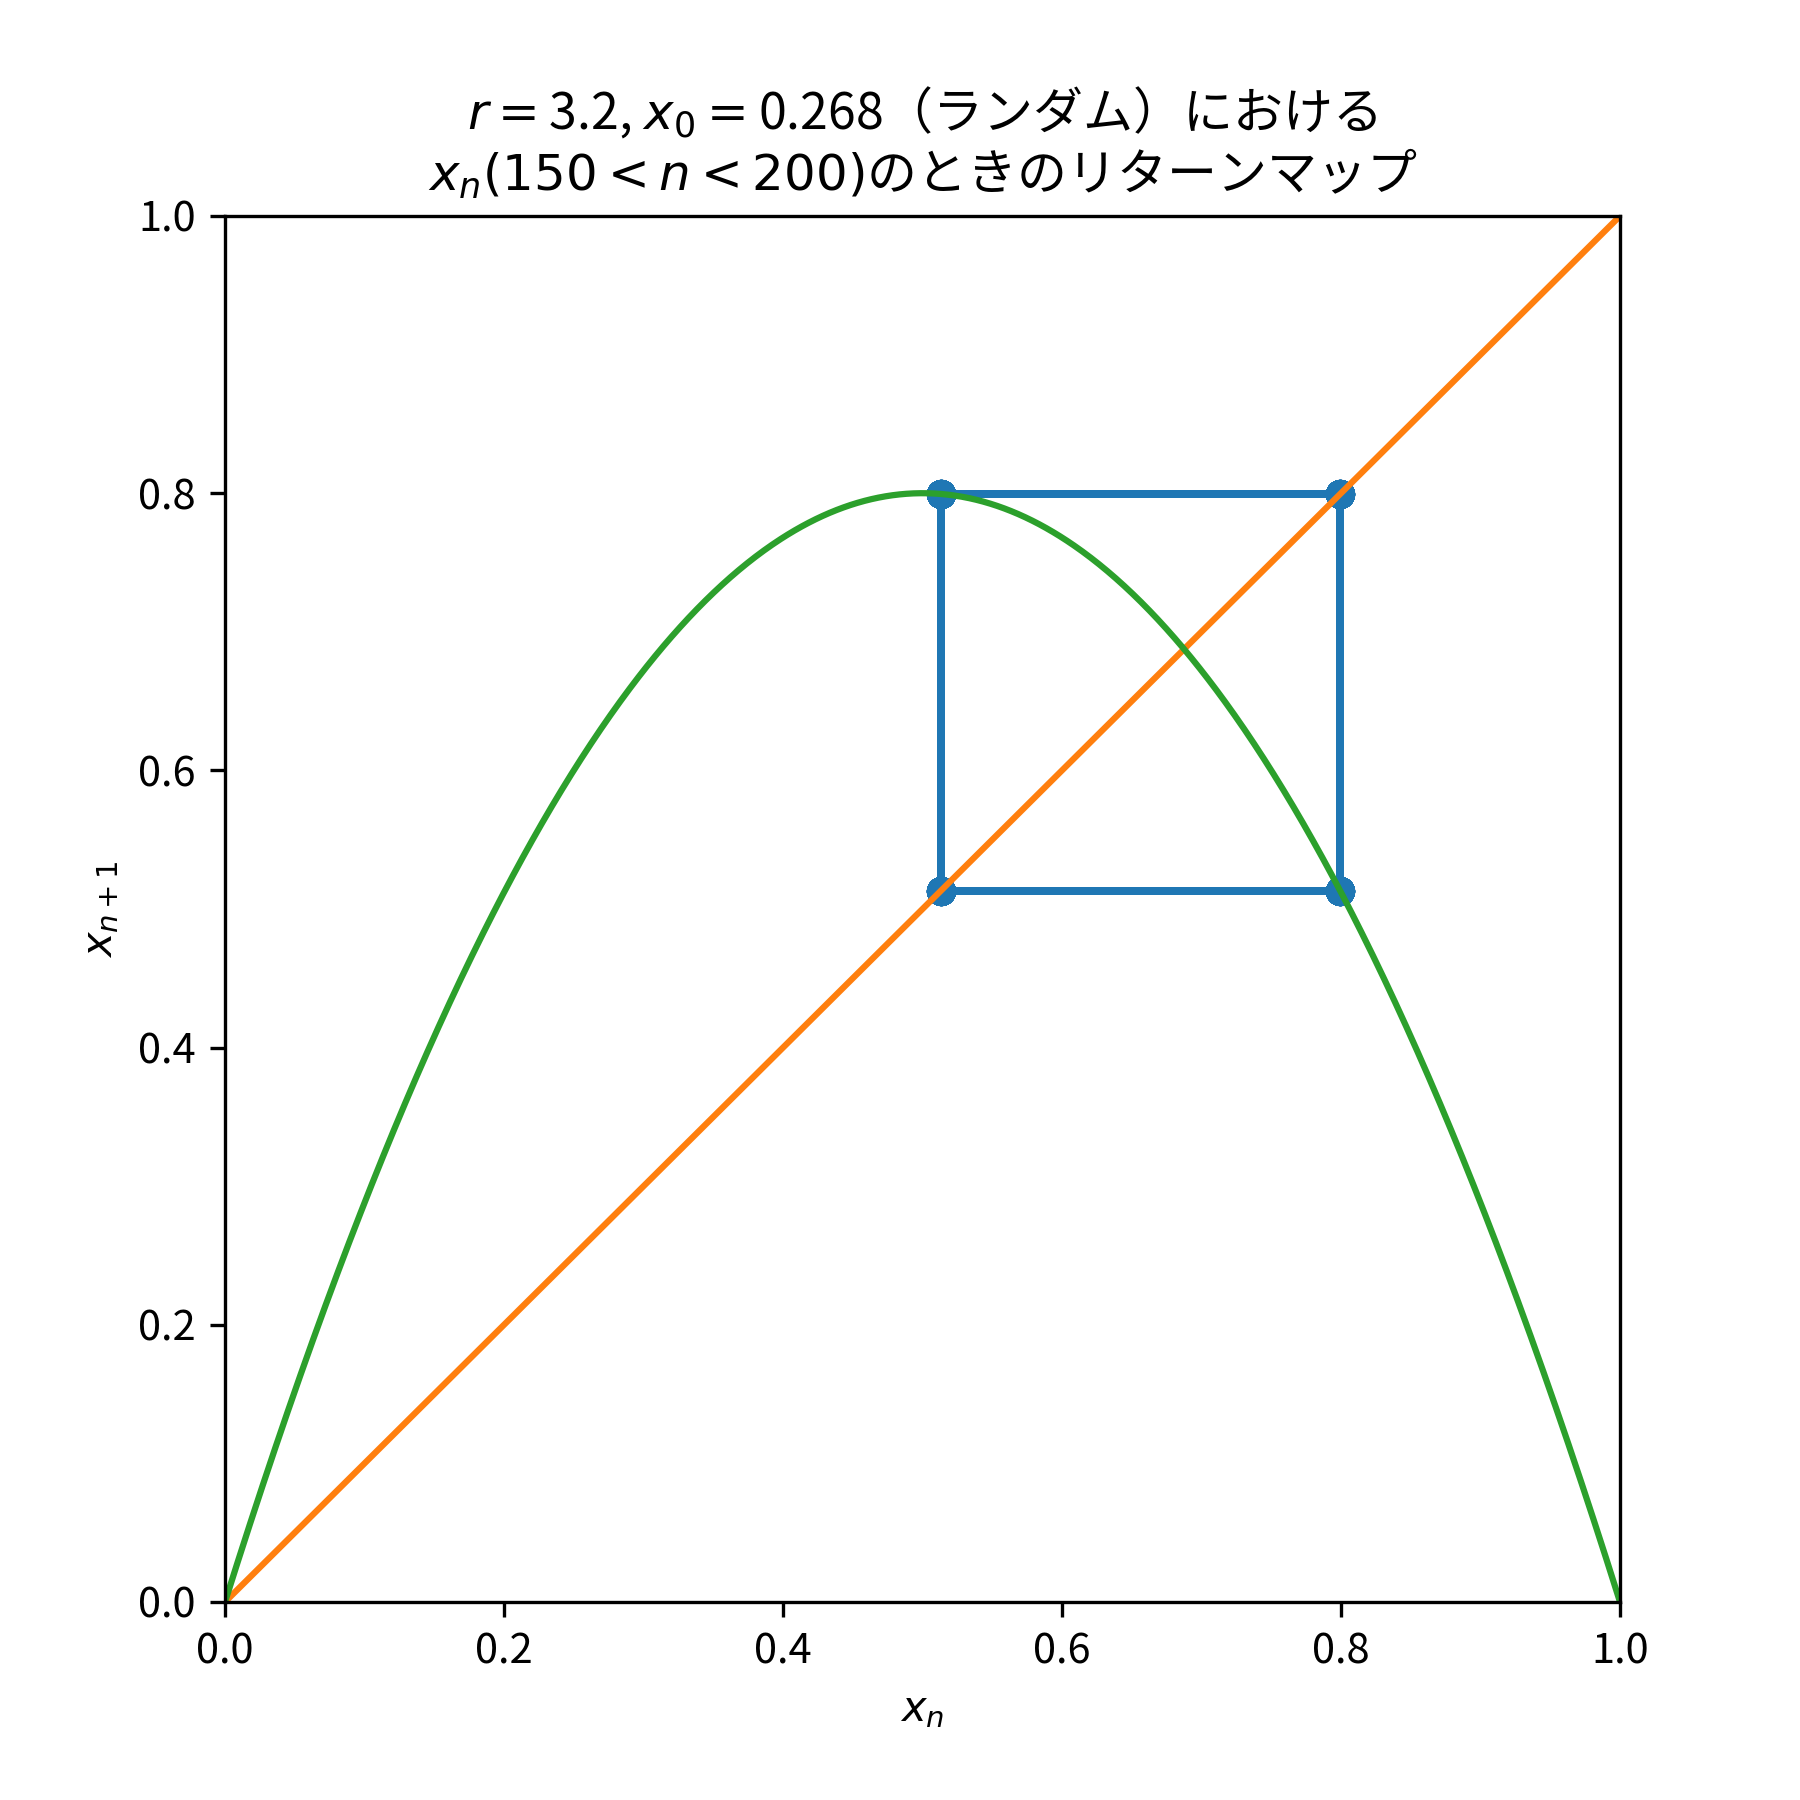
\includegraphics[keepaspectratio, scale=0.3]{images/Problem3/report4_3.png}
    \end{minipage} &
    \begin{minipage}[t]{0.45\hsize}
      \centering
      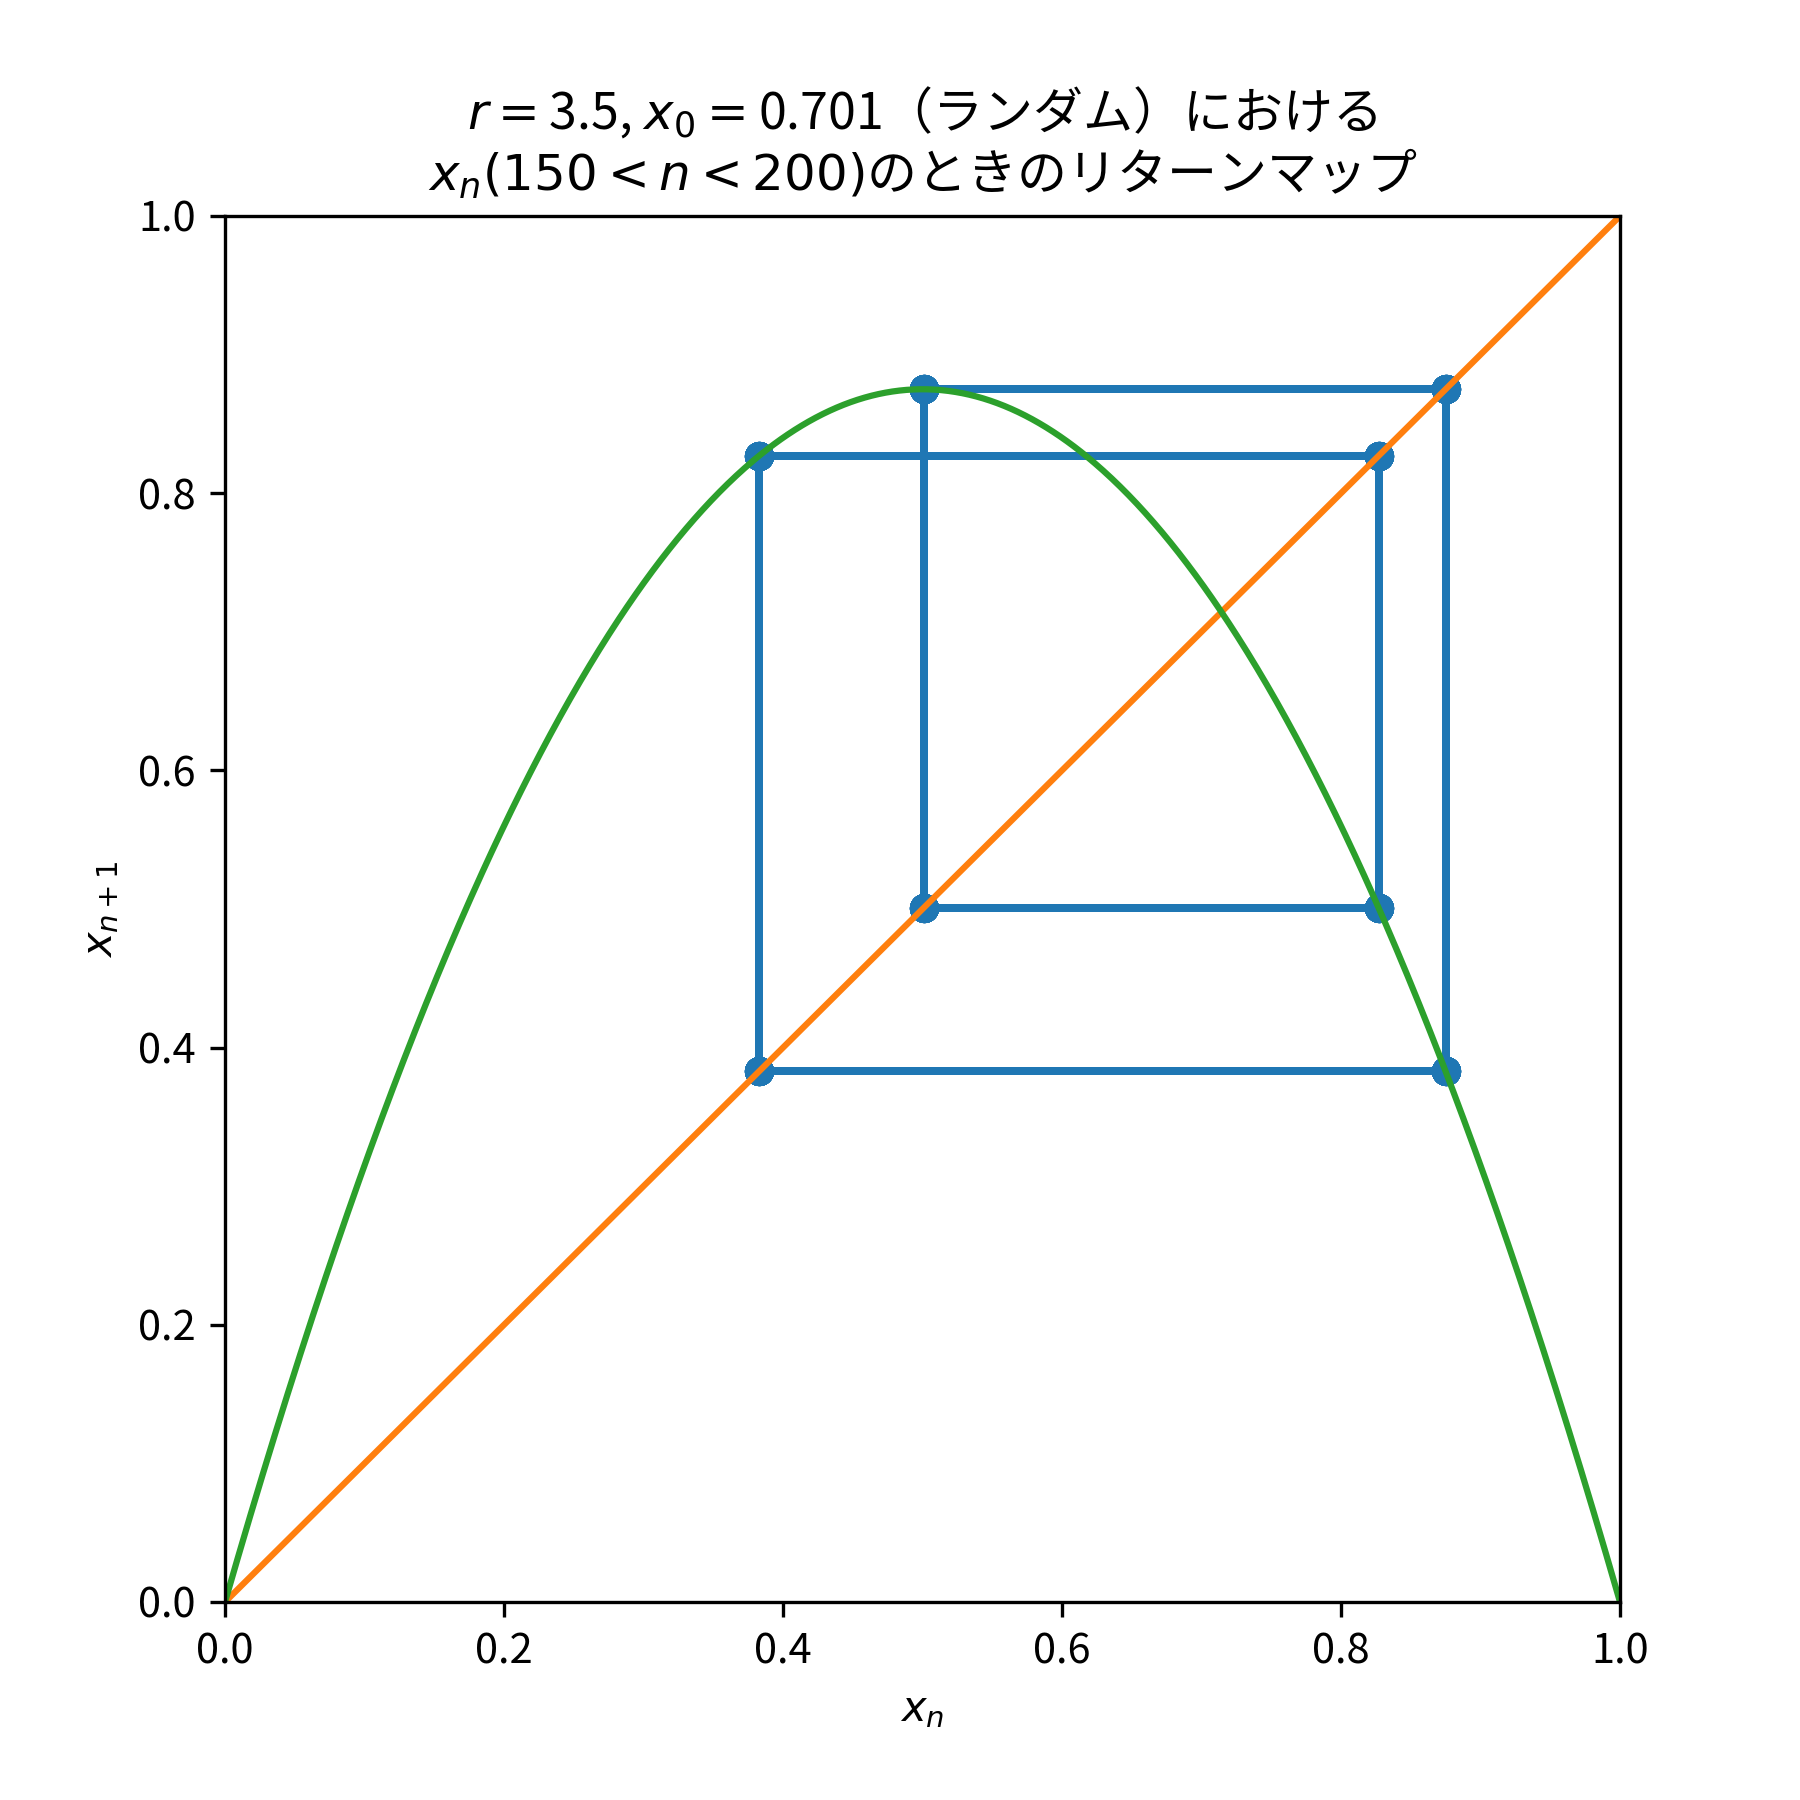
\includegraphics[keepaspectratio, scale=0.3]{images/Problem3/report4_4.png}
    \end{minipage} \\

    \begin{minipage}[t]{0.45\hsize}
      \centering
      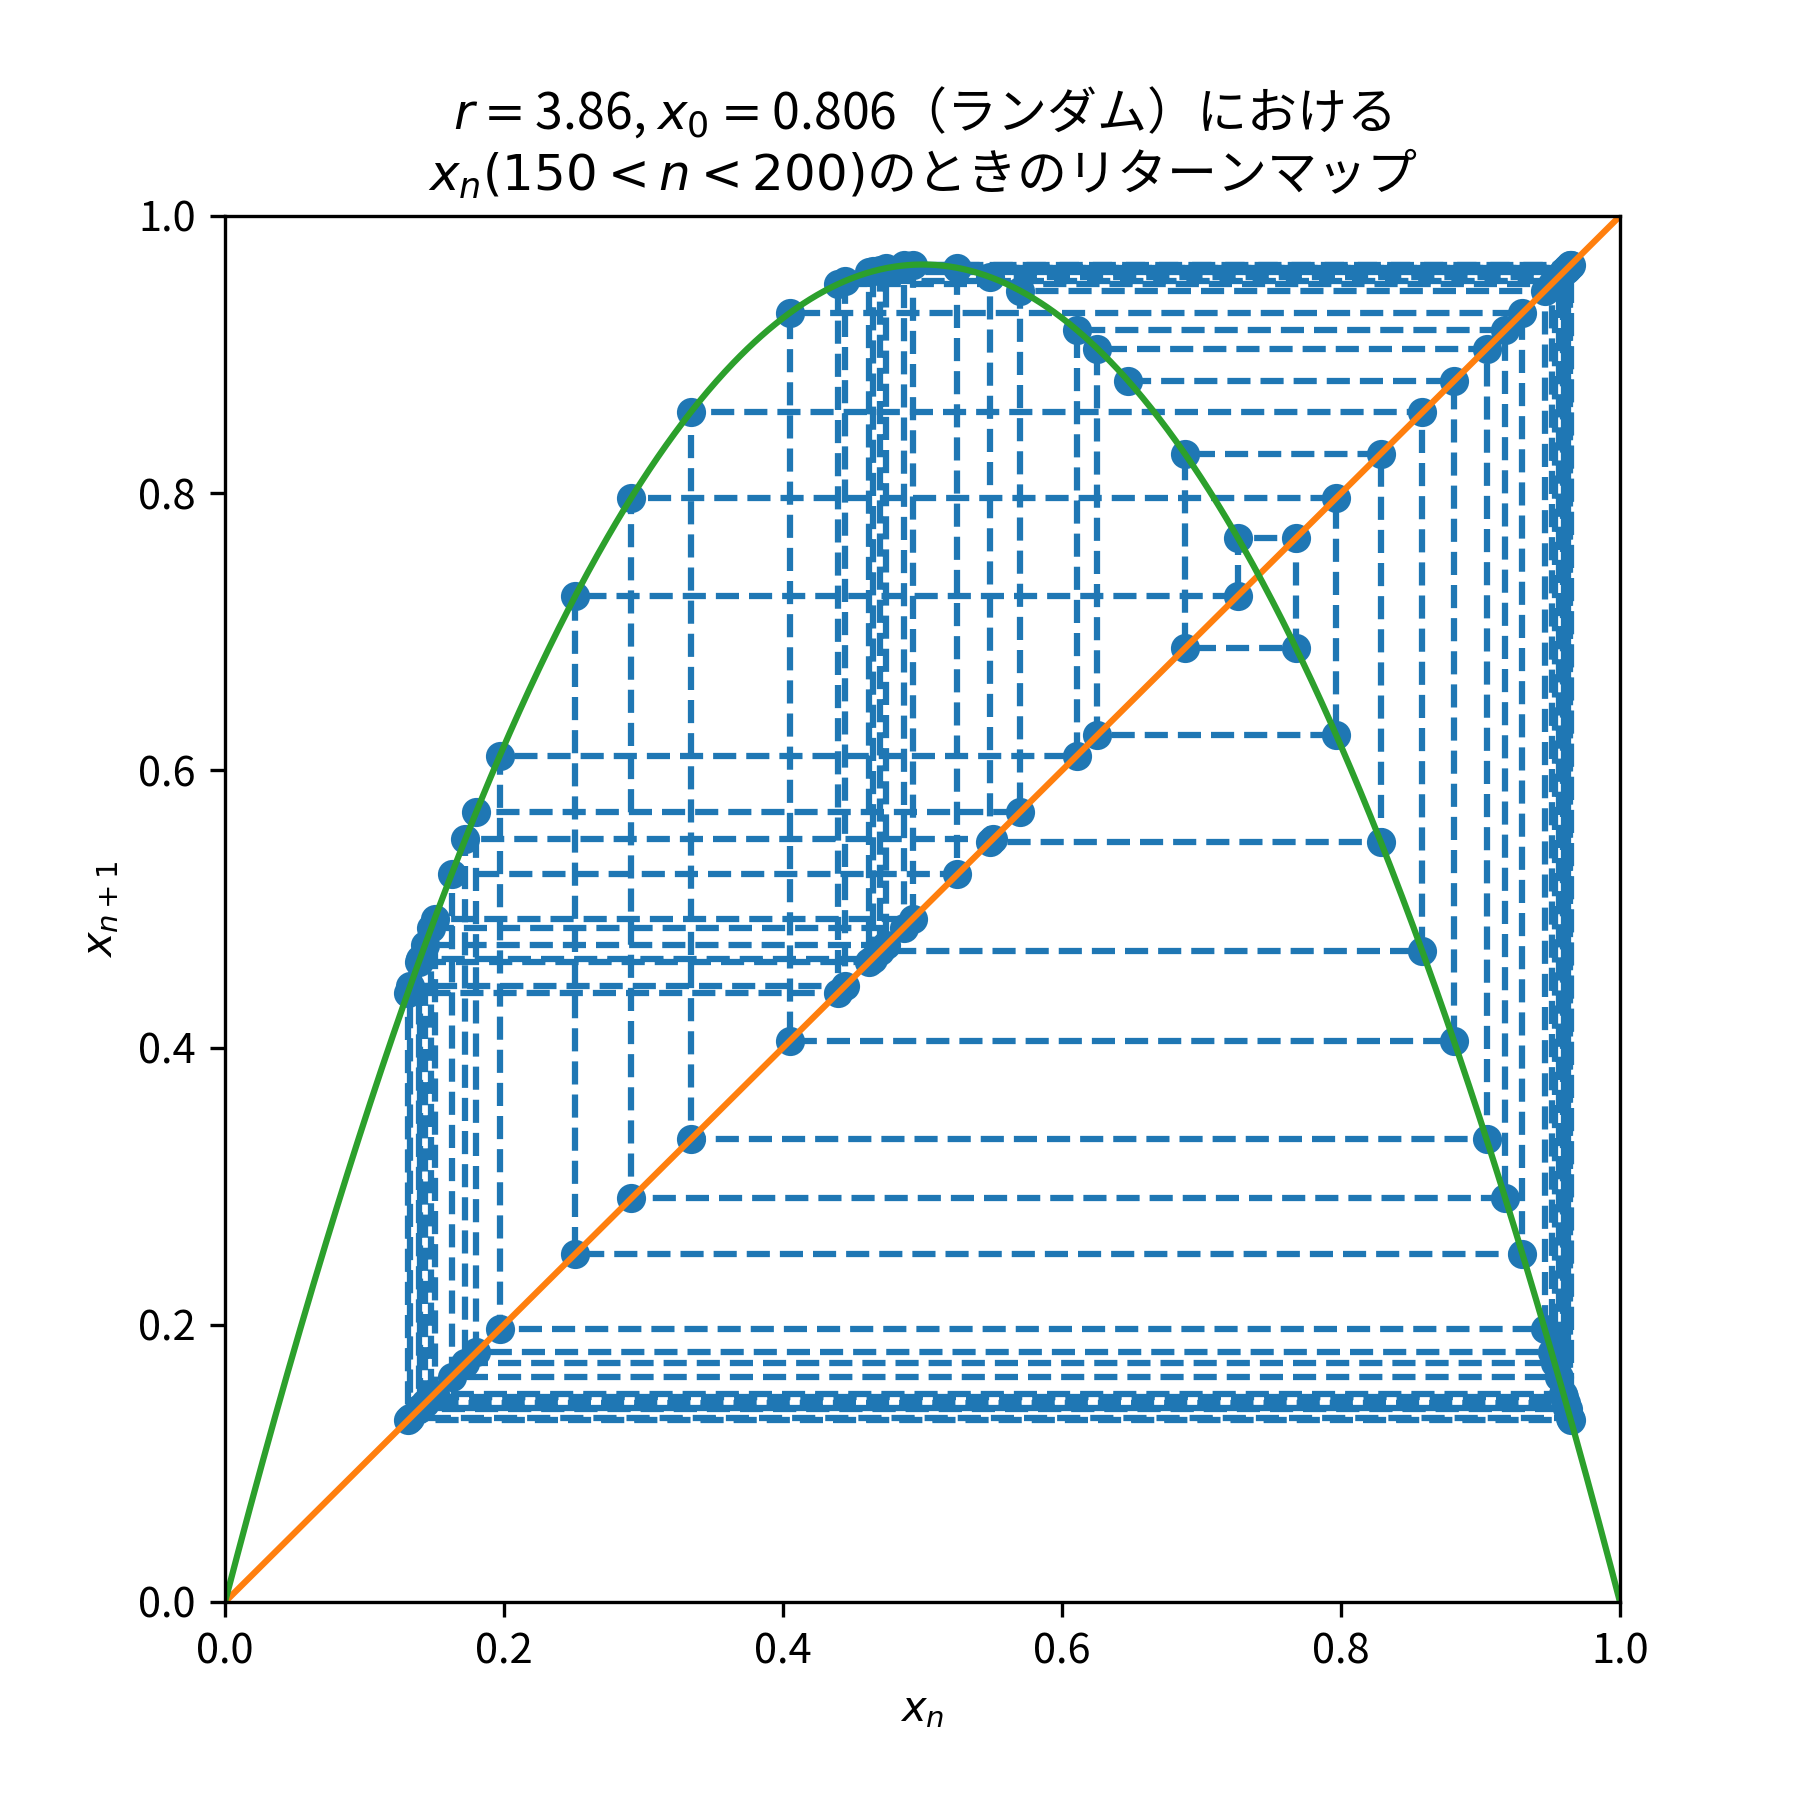
\includegraphics[keepaspectratio, scale=0.3]{images/Problem3/report4_5.png}
    \end{minipage} &
    \begin{minipage}[t]{0.45\hsize}
      \centering
      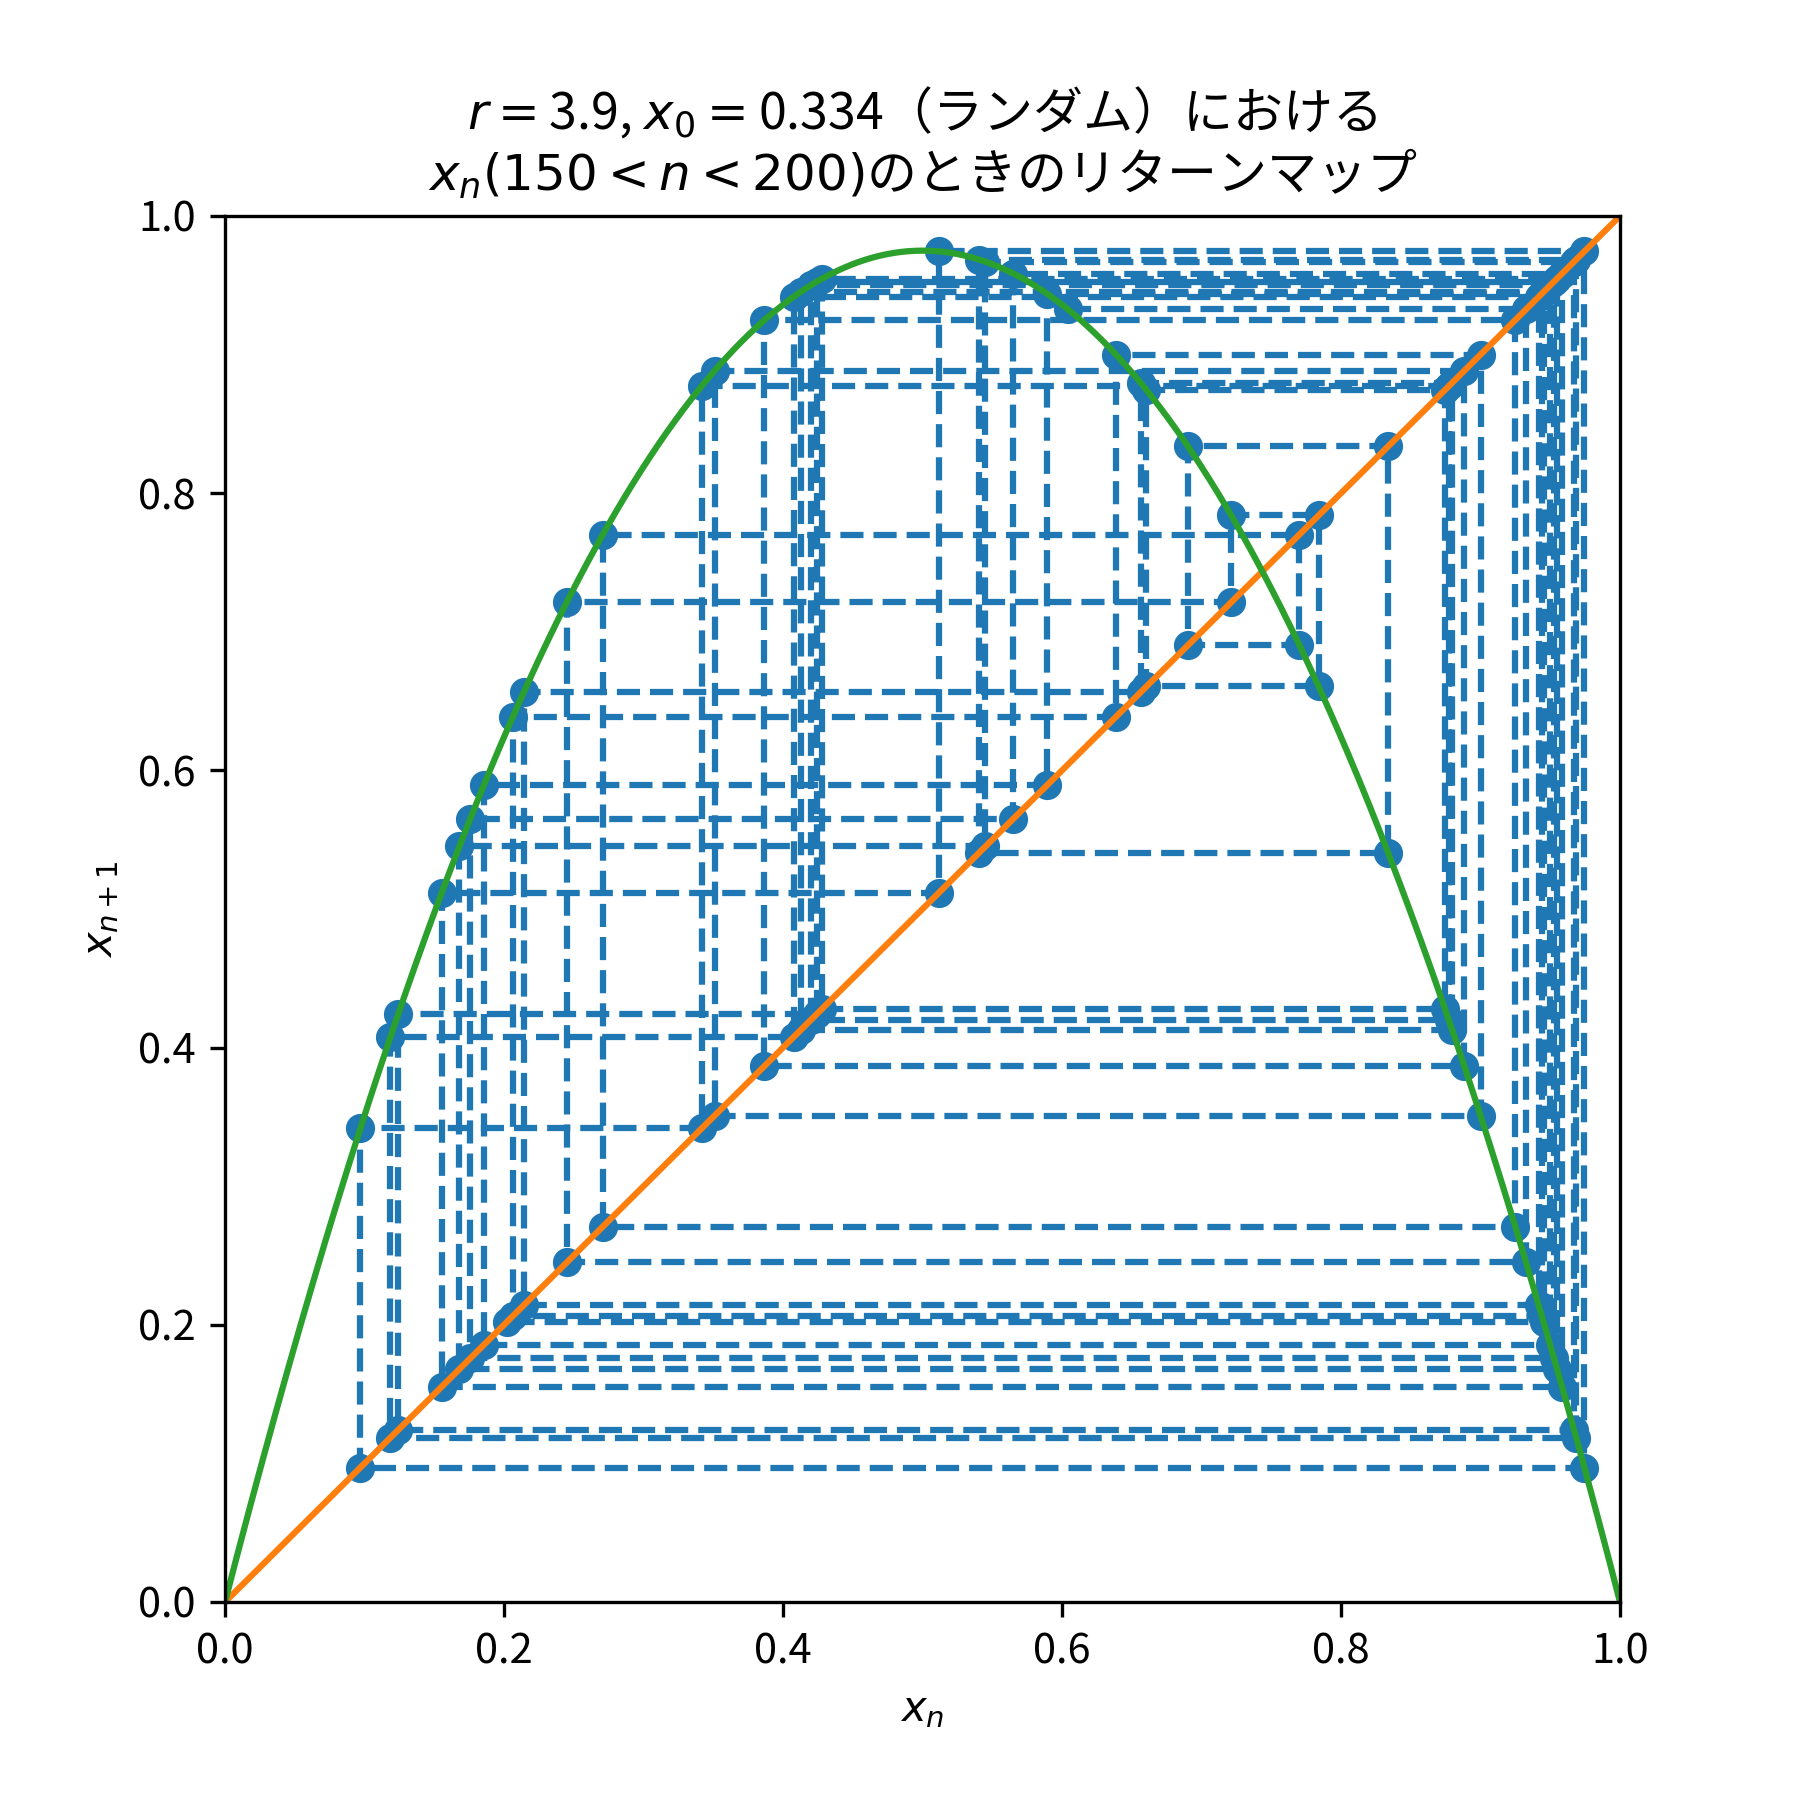
\includegraphics[keepaspectratio, scale=0.3]{images/Problem3/report4_6.png}
    \end{minipage}
  \end{tabular}
\end{figure}
\\
結果:\\
この画像から読み取れた。\\\\
考察:\\
これらの結果から考察することができる。


\subsection{課題2}
$r$ が $1~4$ のときのロジスティク写像の分岐図を描け。また、分岐図の中で3周期の窓が現れている $r$ の範囲を抽出して、グラフを描け。このとき、両グラフとも $r$ は各自適切な刻み幅を設定し、各 $r$ について初期値$x_0$をランダムに与えること。プログラムのソースコードは、 $r$ が $1~4$ のときの分岐図を出力するものと3周期の窓を出力するものとの2つを記載すること。\\
画像:\\
\begin{figure}[htbp]
  \centering
  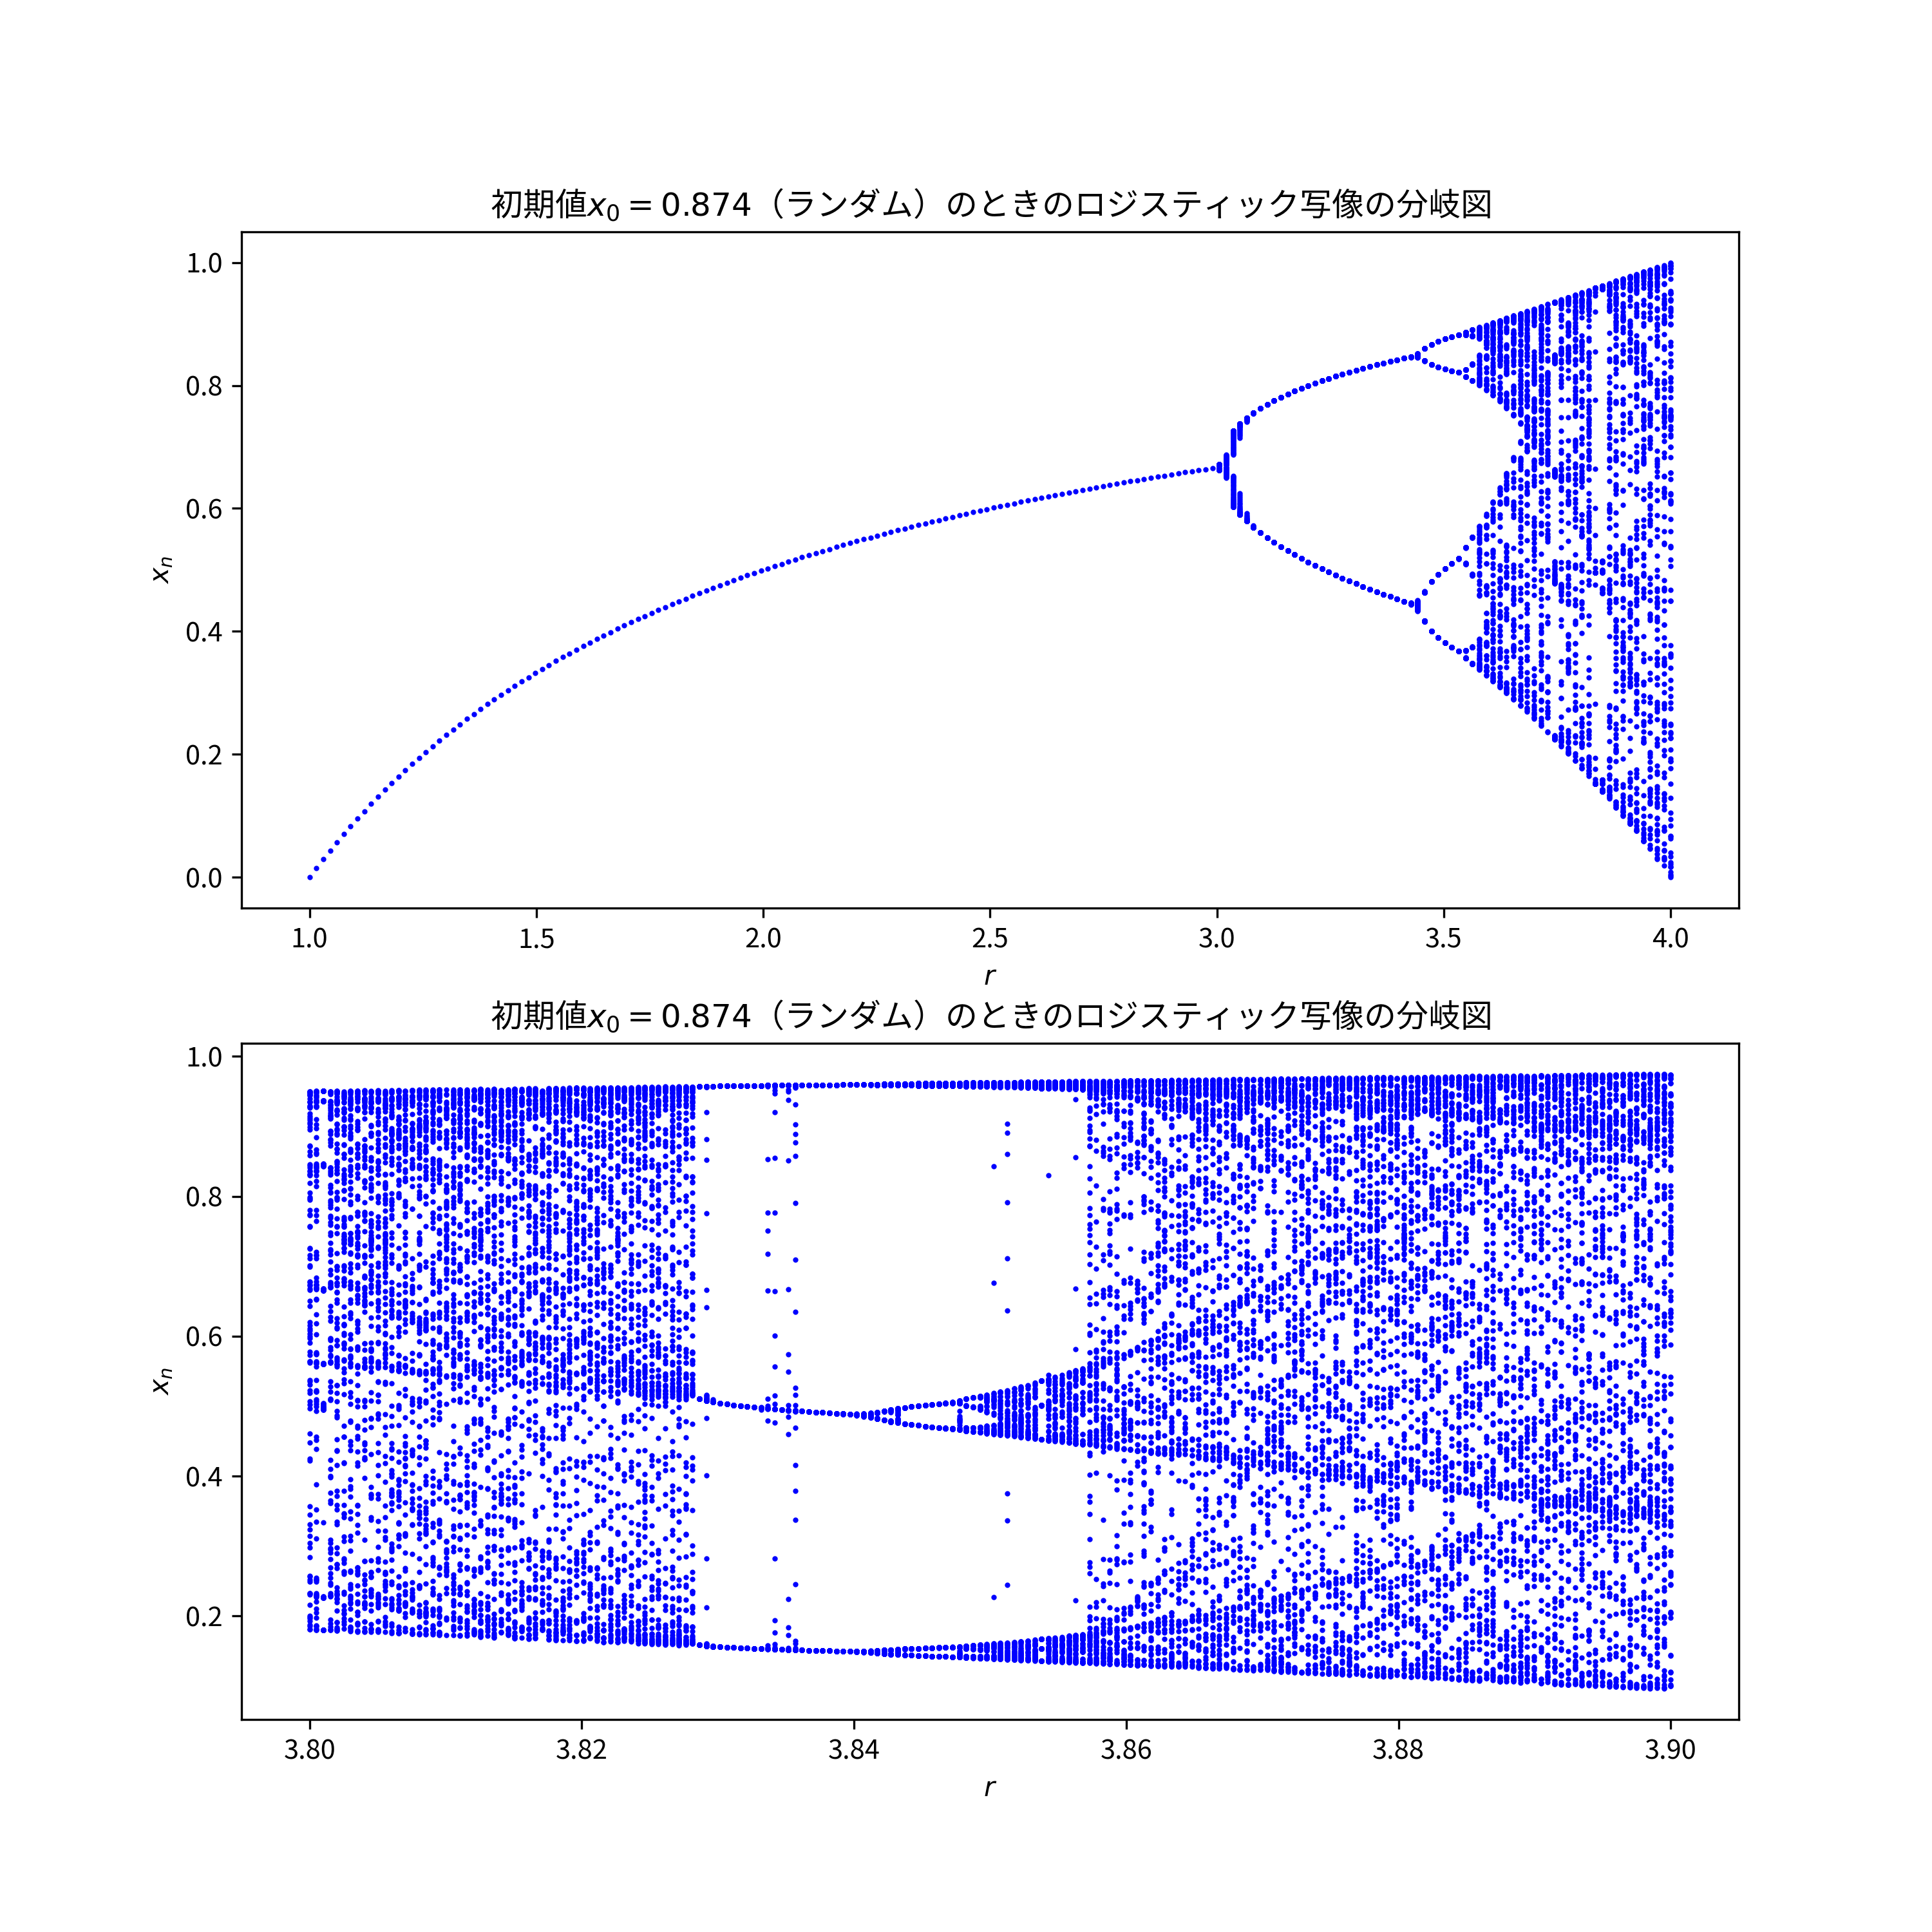
\includegraphics[keepaspectratio, scale=0.6]{images/Problem3/ctest4.png}
\end{figure}
\\
結果:\\
この画像から読み取れた。\\\\
考察:\\
これらの結果から考察することができる。

\subsection{課題3}
課題1と課題2は、各 $r$ ごとに初期値 $x_0$ をランダムに与えているにもかかわらず、 $r$ が $1~3.5$ くらいまでは何度プログラムを実行しても同じようなグラフを描くことができる。一方、 $r$ が $3.5$ よりも大きくなっていくと、プログラムを実行するたびにグラフを一見するだけではわからないような違いが生じる。この理由を前回の課題と初期値鋭敏性という言葉を用いて説明せよ。
\section{レポート課題4}
\subsection{課題1}
リアプノフ指数の $r$ 依存性を示したグラフを描け。但し、初期値をランダムに与え、グラフの横軸は $1 〜 4$ 、縦軸は $-3 〜 1$ までの範囲にすること。 $r$ の刻み幅は、各自適切な値を設定すること。\\


\subsection{課題2}
3周期の窓の領域でのリアプノフ指数の $r$ 依存性を示したグラフを描け。但し、初期値をランダムに与え、グラフの縦軸は $-1 〜 0.4$ までの範囲にすること。 $r$ の範囲および刻み幅は、各自適切な値を設定すること。


\subsection{課題3}
ロジスティック写像についてまとめ、これまでに出題された全て (4 回分 ) の結果について考察せよ。分量は A4 用紙 1 〜 4 枚程度を目安としてください。\\\\
 レポート課題1の考察は、ロジスティック写像は $r$ の値を変化させていくことで非周期性を満たすものと満たさないものがあると考察した。レポート課題1では初期値は $x_0 = 0.7$ に固定して $r$ の値によってどのような軌道になっていくかを比較した。それぞれの結果から、 $x_{n+1} = r(1 −x_n)x_n$ と $x_{n+1} = x_n$、 $x_0$ の位置関係と $r$ の値が収束、発散と関係していると考察した。\\
 レポート課題2の考察は、 $r = 3.86, r = 3.90$ のときは初期値 $x_0$ の小さい変化によって $x_{200}$ と $x_n (150 < n < 200)$ が大きく変化することが考察できる。レポート課題2では、初期値 $x_0$ の変化によって $x_{200}$ がどのようになっていくかを調べる問題になっていた。また、レポート課題2で比較した $r$ はレポート課題1と同様のものとなっている。レポート課題2の結果から非周期性を満たすかどうかは $r$ によって決まっていくことがより強く考察することができた。また、今回は初期値 $x_0$ を変化させていたので非周期性を満たすときの $x_{200}$ の挙動がどうなっていくか確認することができた。非周期性を満たすときの $x_{200}$ の値には規則性が見られることはなかった。これにより $r = 3.86, r = 3.90$ のときには初期値鋭敏性の要素が含まれていることが考察できた。初期値鋭敏性とは、初期状態での小さな差があると時間経過に応じて指数関数的にその差が増加するというカオスの条件のひとつである。\\
 レポート課題3は、添付している画像のランダムの値の他にもいくつかの値で課題1を実行してみたが、やはり $r = 1.50, r = 2.60, r = 3.20, r = 3.50$ のときはある値を反復し $r = 3.86, r = 3.90$ のときは値が定まることなく変化していた。これらの結果から $r = 3.86, r = 3.90$ のときはカオスの条件のひとつである非周期性が満たされていると考察することができる。また課題2の結果からこれらの結果から初期値 $x_0$ ではなく $r$ の値がカオスの条件と関係していると考察することができる。\\
 レポート課題4\\
\section{特別課題}
\subsection{Mandelbrot 集合}
\begin{figure}[htbp]
  \centering
  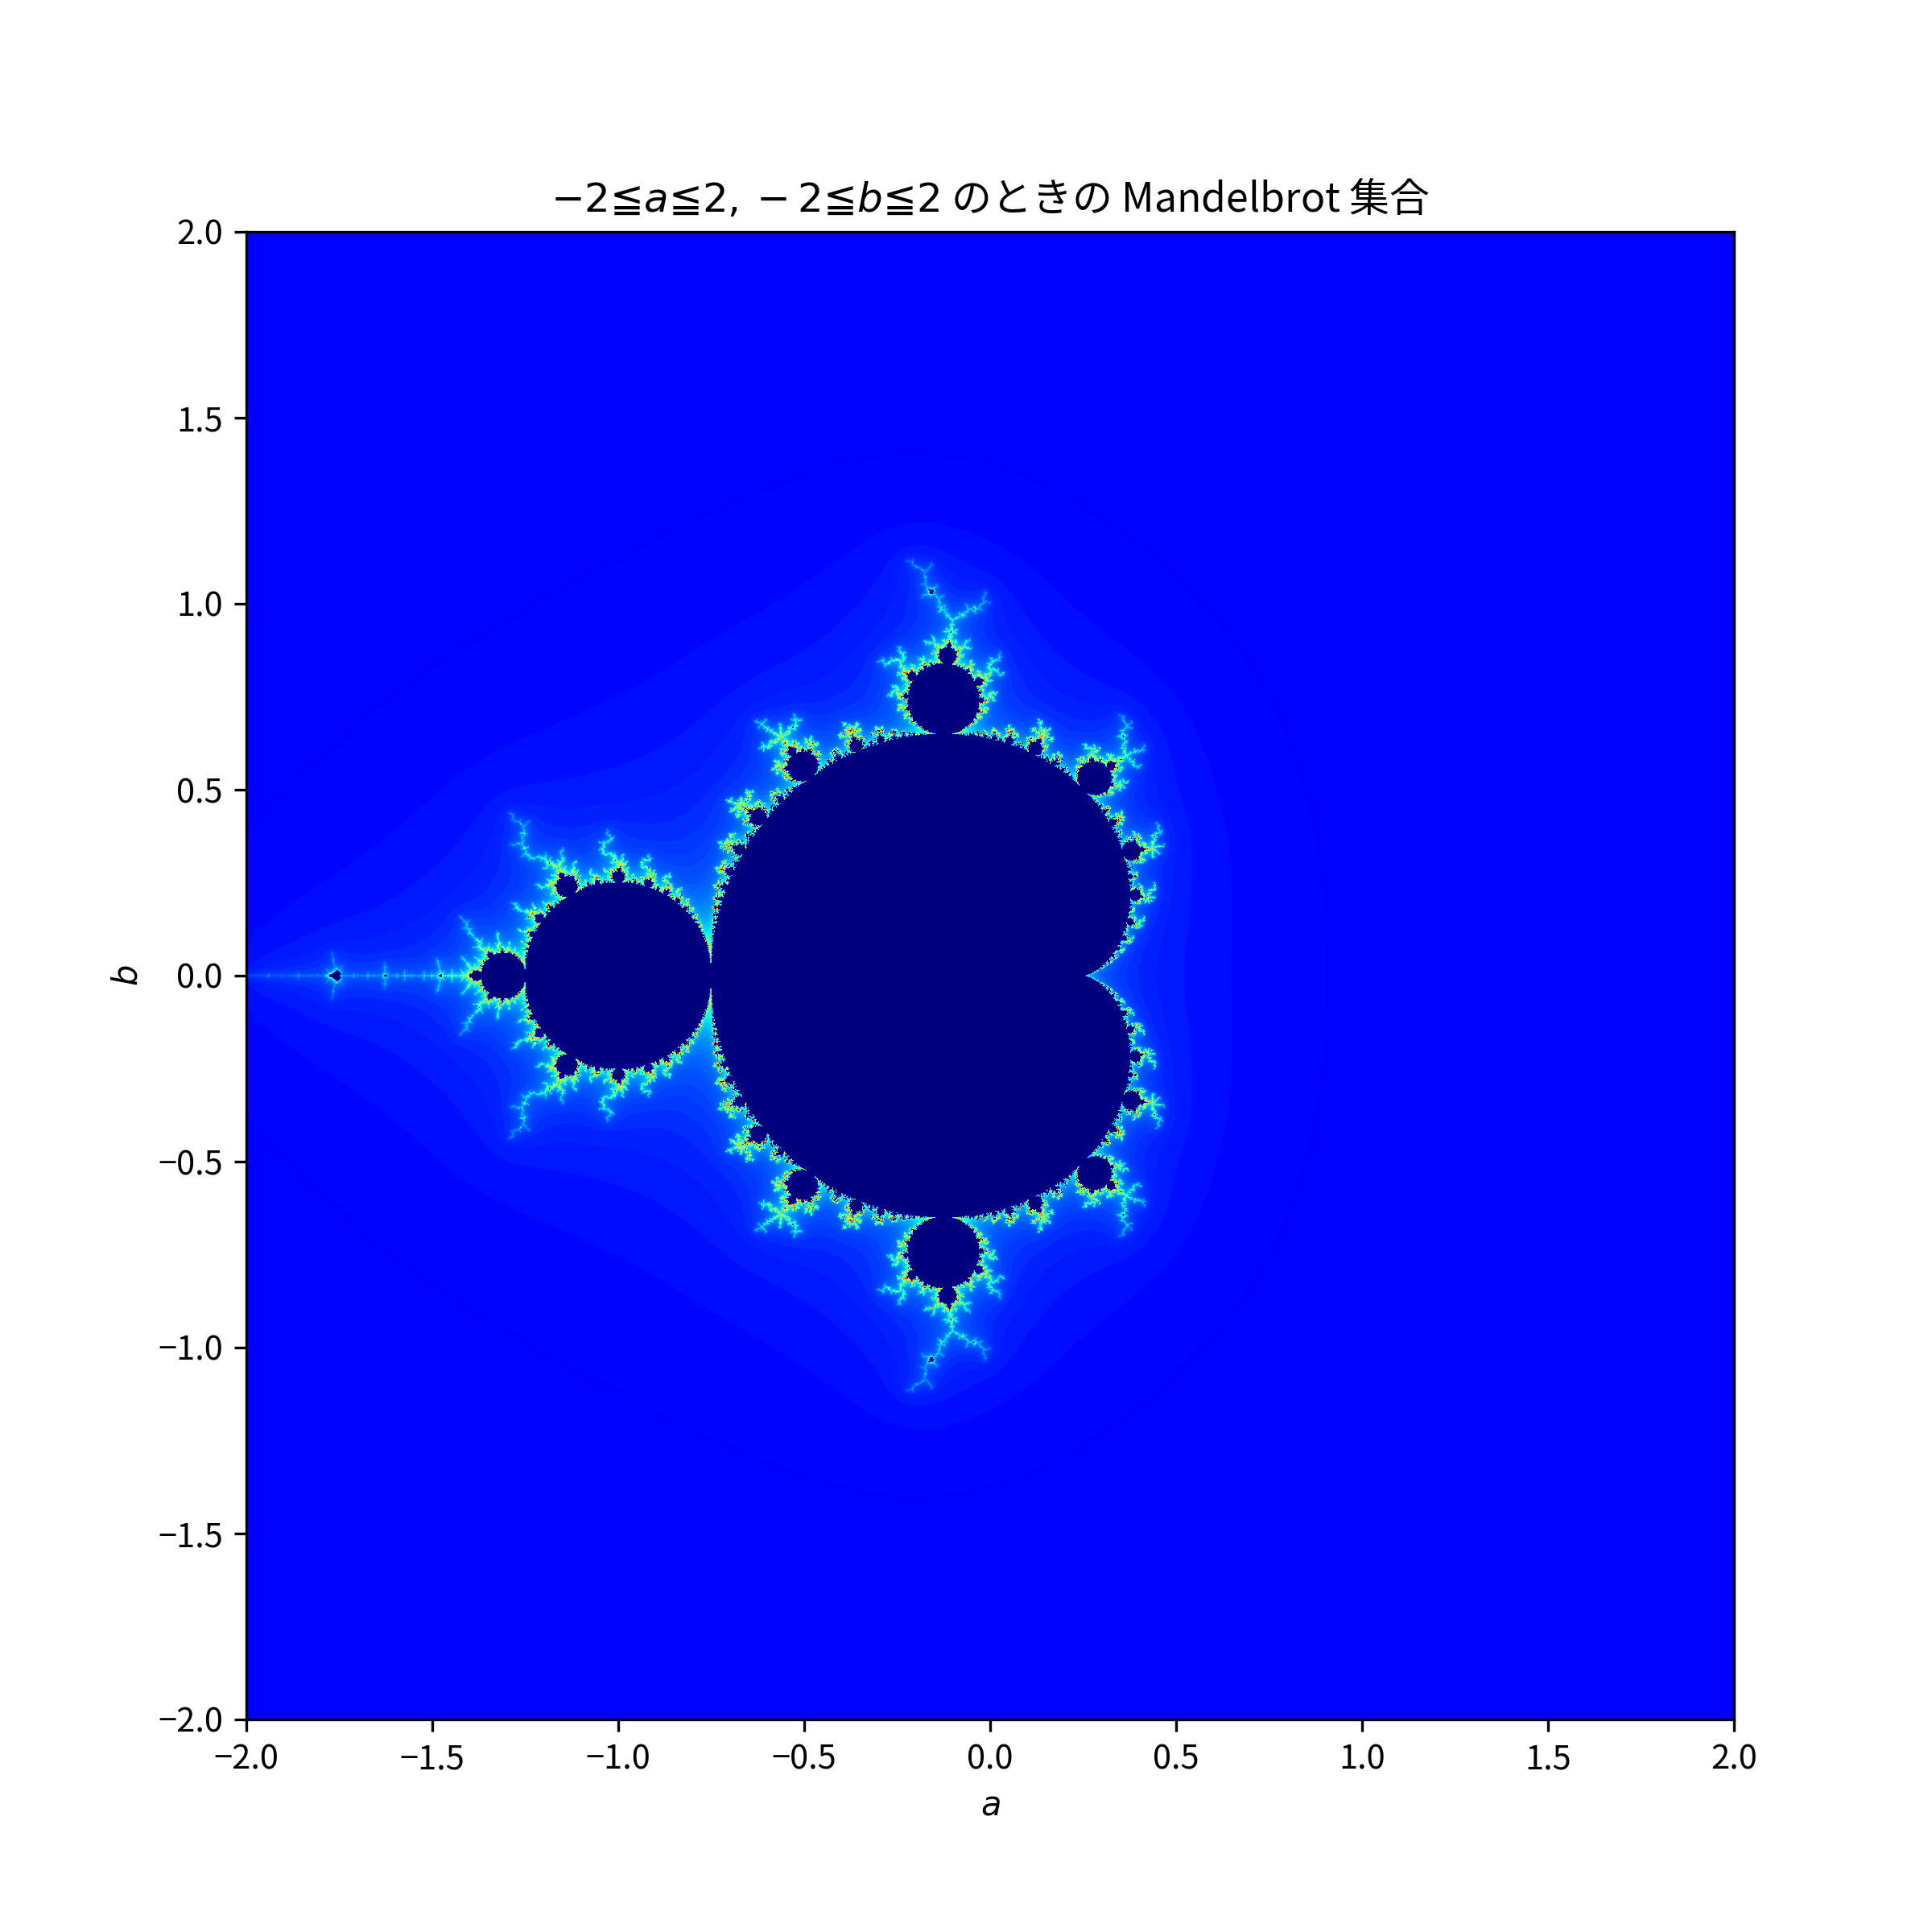
\includegraphics[keepaspectratio, scale=0.8]{images/OtherProblem/ctest5_1.png}
\end{figure}
解説:\\
今回はPythonを用いて複素数の計算を簡略化しマンデルブロ集合をプロットした。まず、$a, b$ それぞれの範囲での漸化式を計算し、それを複素数平面上にプロットした。\\
\begin{lstlisting}[caption=mandelbrot.py]
  import numpy as np
  import matplotlib
  from matplotlib import pyplot as plt
  from matplotlib.colors import Normalize                     # カラーマップを自在に操作するために必要
  from numba import jit                                       # 計算の高速化


  # 日本語フォント用(Linux)
  matplotlib.rc('font', family='Noto Sans CJK JP')
  '''
  # 日本語フォント用(Windows)
  matplotlib.rc('font', family='MS Gothic')
  '''

  @jit
  def mandelbrot(a, b, n_max):
      "複素数を用いてマンデルブロ集合の座標を求める関数"
      a_num, b_num = np.meshgrid(a, b)
      n_grid = len(a_num.ravel())                             # 組み合わせの総数
      z = np.zeros(n_grid)                                    # マンデルブロ集合のデータ格納用空配列


      for i in range(n_grid):
          c = complex(a_num.ravel()[i], b_num.ravel()[i])     # c = a + bi
          n = 0
          z0 = complex(0, 0)
          while np.abs(z0) < np.inf and not n == n_max:
              z0 = z0 ** 2 + c                                # 漸化式を計算
              n += 1
          
          if n == n_max:
              z[i] = 0
          else:
              z[i] = n
      z = np.reshape(z, a_num.shape)                          # 2次元配列に変換
      z = z[::-1]                                             # imshow()で上下逆になるので上下反転
      return z


  a = np.linspace(-2, 2, 2000)
  b = np.linspace(-2, 2, 2000)
  z = mandelbrot(a, b, 100)
  file_path = "複雑系科学演習/Week6/images/"
  plt.figure(figsize=(8, 8))
  plt.xlabel('$a$')
  plt.ylabel('$b$')
  plt.title("$-2 \leqq a \leqq 2, -2 \leqq b \leqq 2$ のときの Mandelbrot 集合")
  plt.imshow(z, cmap='jet', norm=Normalize(vmin=0, vmax=100), extent=[-2, 2, -2, 2])
  plt.savefig(file_path + "ctest5_1", dpi=300)
  plt.show()
\end{lstlisting}

\newpage
\subsection{Julia 集合}
\begin{figure}[htbp]
  \centering
  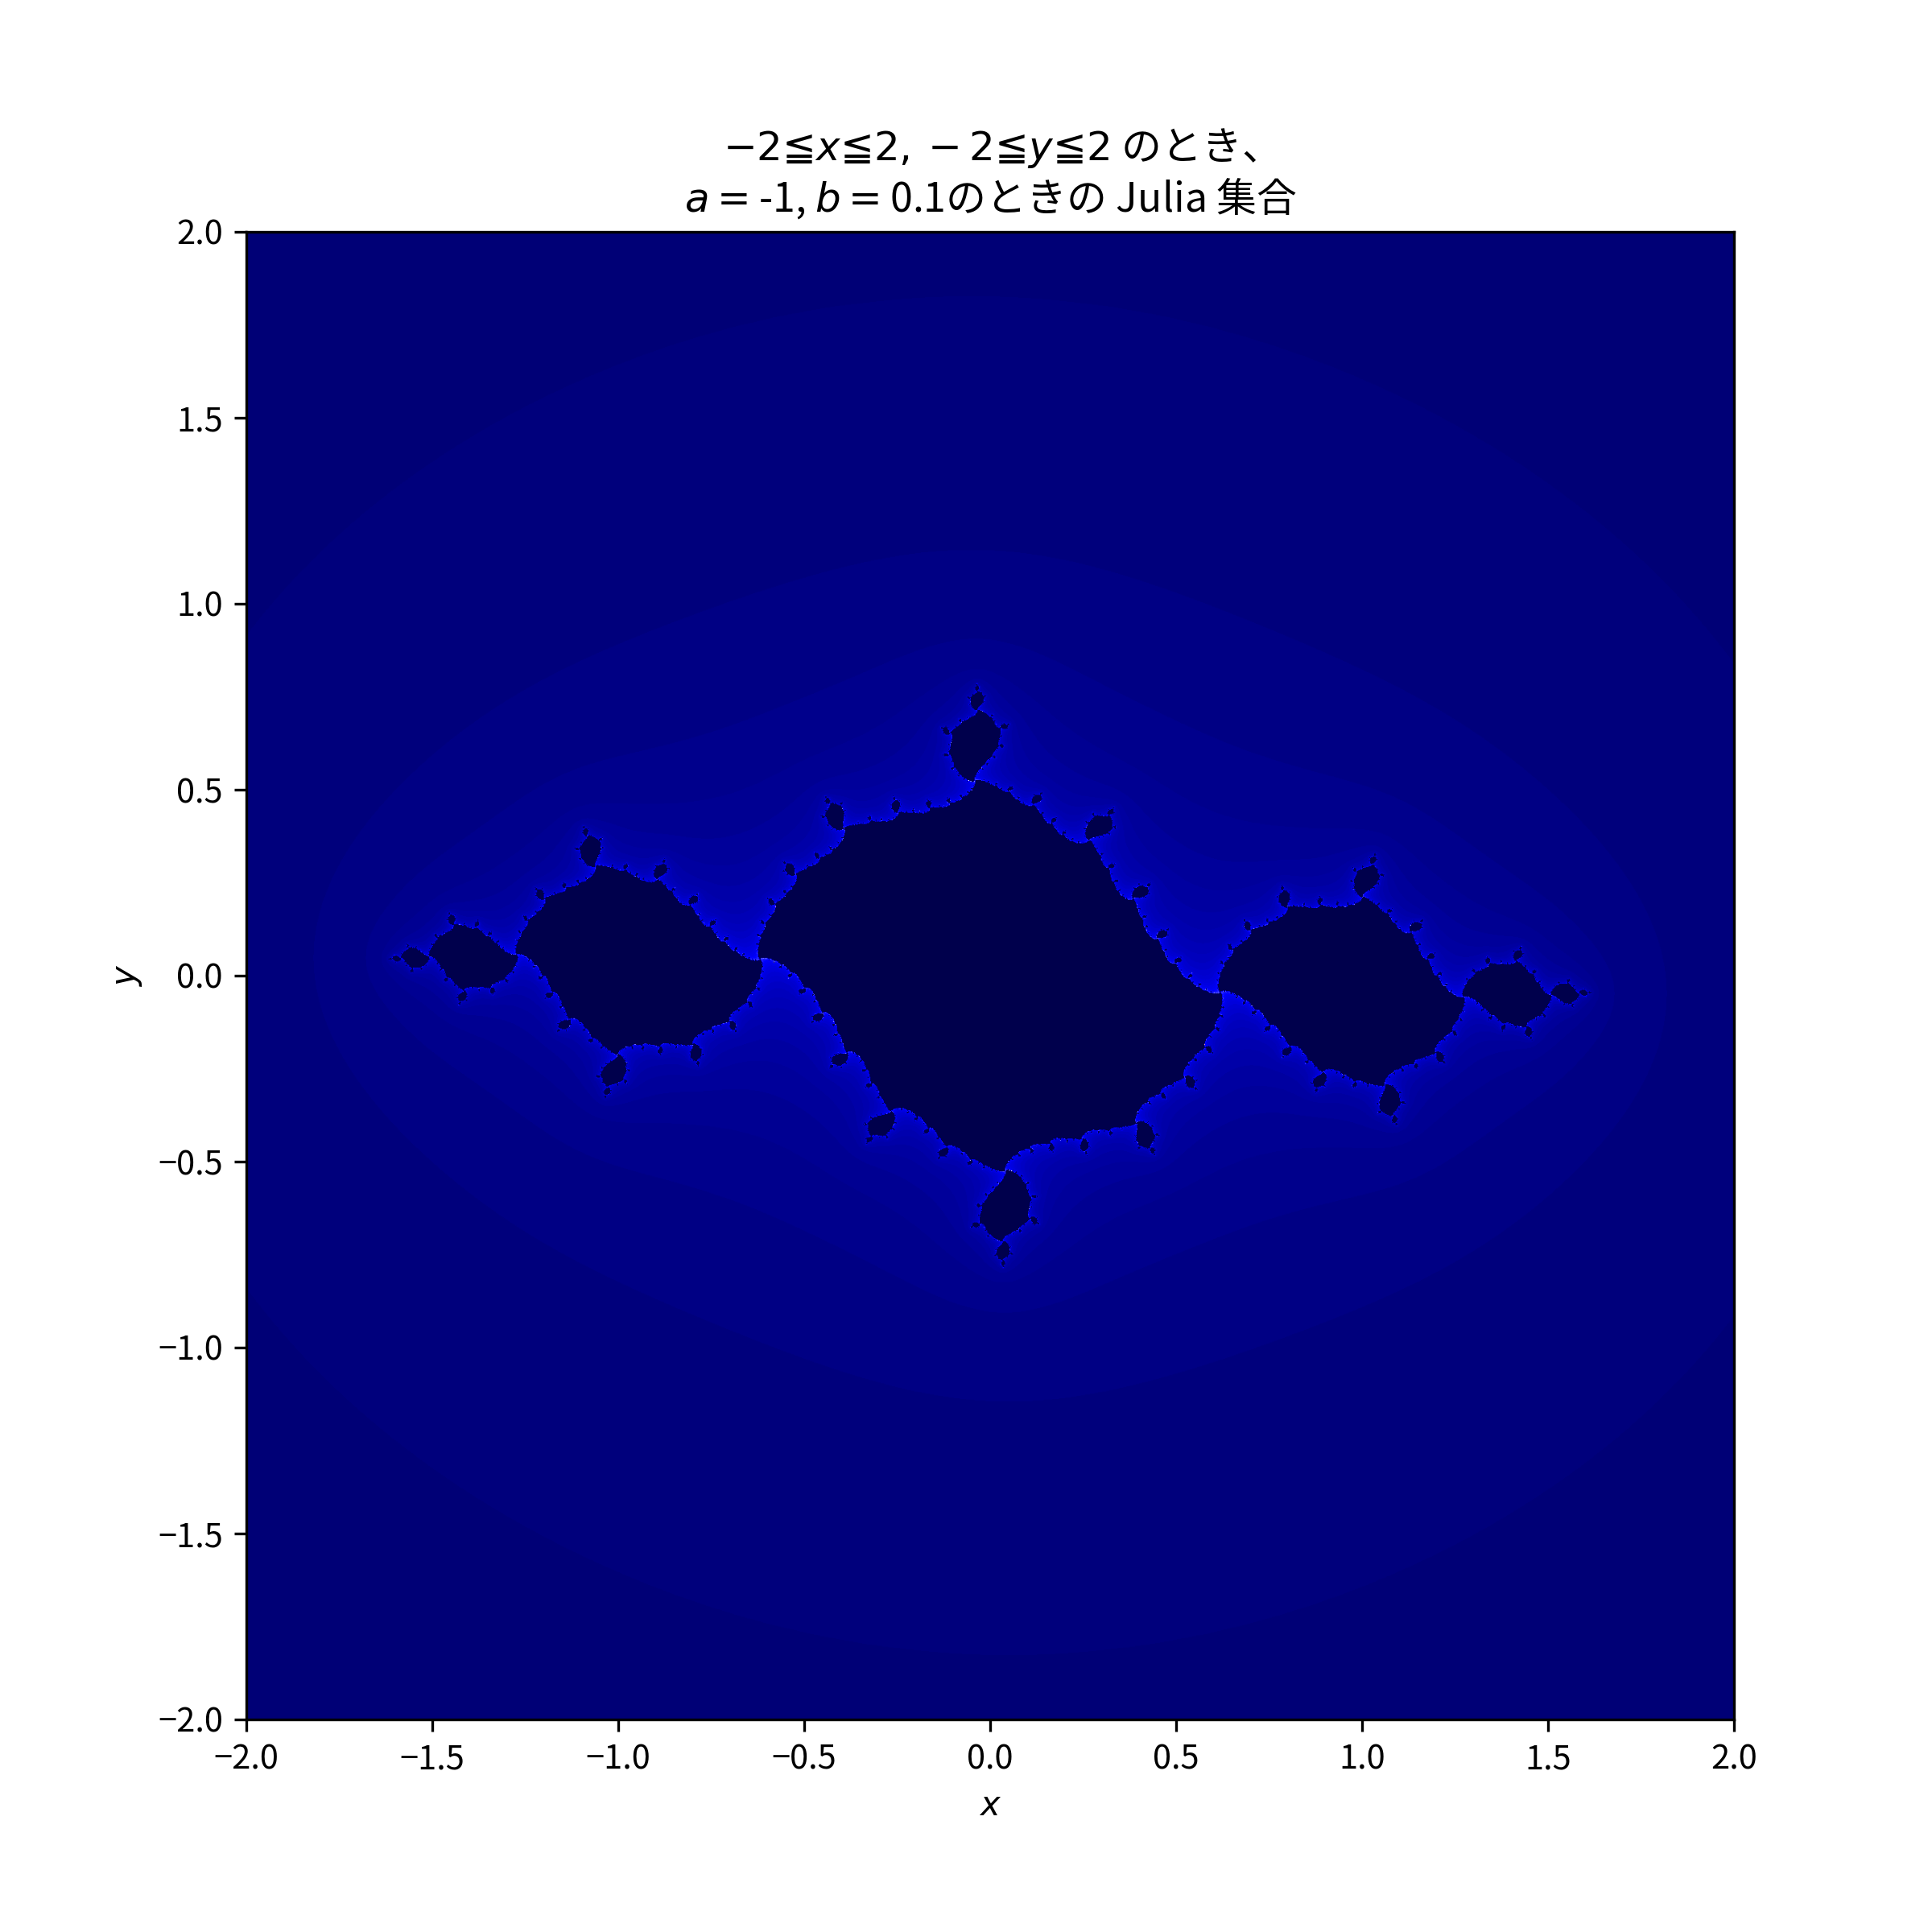
\includegraphics[keepaspectratio, scale=0.8]{images/OtherProblem/ctest5_2.png}
\end{figure}
解説:\\
ジュリア集合はマンデルブロ集合と似たような集合である。マンデルブロ集合では、$z_0 = 0$ として $c$ を変化させてきたがジュリア集合は逆の $c$ を固定し $z_0$ を変化させていく集合である。\\
\begin{lstlisting}[caption=julia.py]
  import numpy as np
  from matplotlib import pyplot as plt
  from matplotlib.colors import Normalize                 # カラーマップ操作
  from numba import jit                                   # 計算の高速化
  from random import uniform
  import matplotlib

  # 日本語フォント用(Linux)
  matplotlib.rc('font', family='Noto Sans CJK JP')
  '''
  # 日本語フォント用(Windows)
  matplotlib.rc('font', family='MS Gothic')
  '''

  @jit                                                    # 計算の高速化
  def julia(x, y, n_max, a, b):
      x_num, y_num = np.meshgrid(x, y)                    # xとyの組み合わせを計算
      n_grid = len(x_num.ravel())                         # 組み合わせの総数
      z = np.zeros(n_grid)                                # ジュリア集合のデータ格納用空配列

      for i in range(n_grid):
          c = complex(a, b)                               # c = a + bi

          n = 0
          z0 = complex(x_num.ravel()[i], y_num.ravel()[i])

          while np.abs(z0) < 1e20 and not n == n_max:
              z0 = z0 ** 2 + c                            # 漸化式を計算
              n += 1
          if n == n_max:
              z[i] = 0
          else:
              z[i] = n
      z = np.reshape(z, x_num.shape)                      # 2次元配列(画像表示用)に変換
      z = z[::-1]                                         # imshow()で上下逆になるので上下反転
      return z


  x = np.linspace(-2, 2, 2000)
  y = np.linspace(-2, 2, 2000)
  n_max = 100

  a = -1
  b = 0.1
  z = julia(x, y, n_max, a, b)
  file_path = "複雑系科学演習/Week6/images/"
  plt.figure(figsize=(8, 8))
  plt.xlabel('$x$')
  plt.ylabel('$y$')
  plt.title("$-2 \leqq x \leqq 2, -2 \leqq y \leqq 2$ のとき、\n" +\
      "$a = ${0}, $b = ${1}のときの Julia 集合".format(round(a, 3), round(b, 3)))

  plt.imshow(z, cmap='seismic', norm=Normalize(vmin=0, vmax=n_max), extent=[-2, 2, -2, 2])
  plt.savefig(file_path + "ctest5_2", dpi=300)
  plt.show()
\end{lstlisting}

\newpage
\subsection{Koch 曲線}
\begin{figure}[htbp]
  \centering
  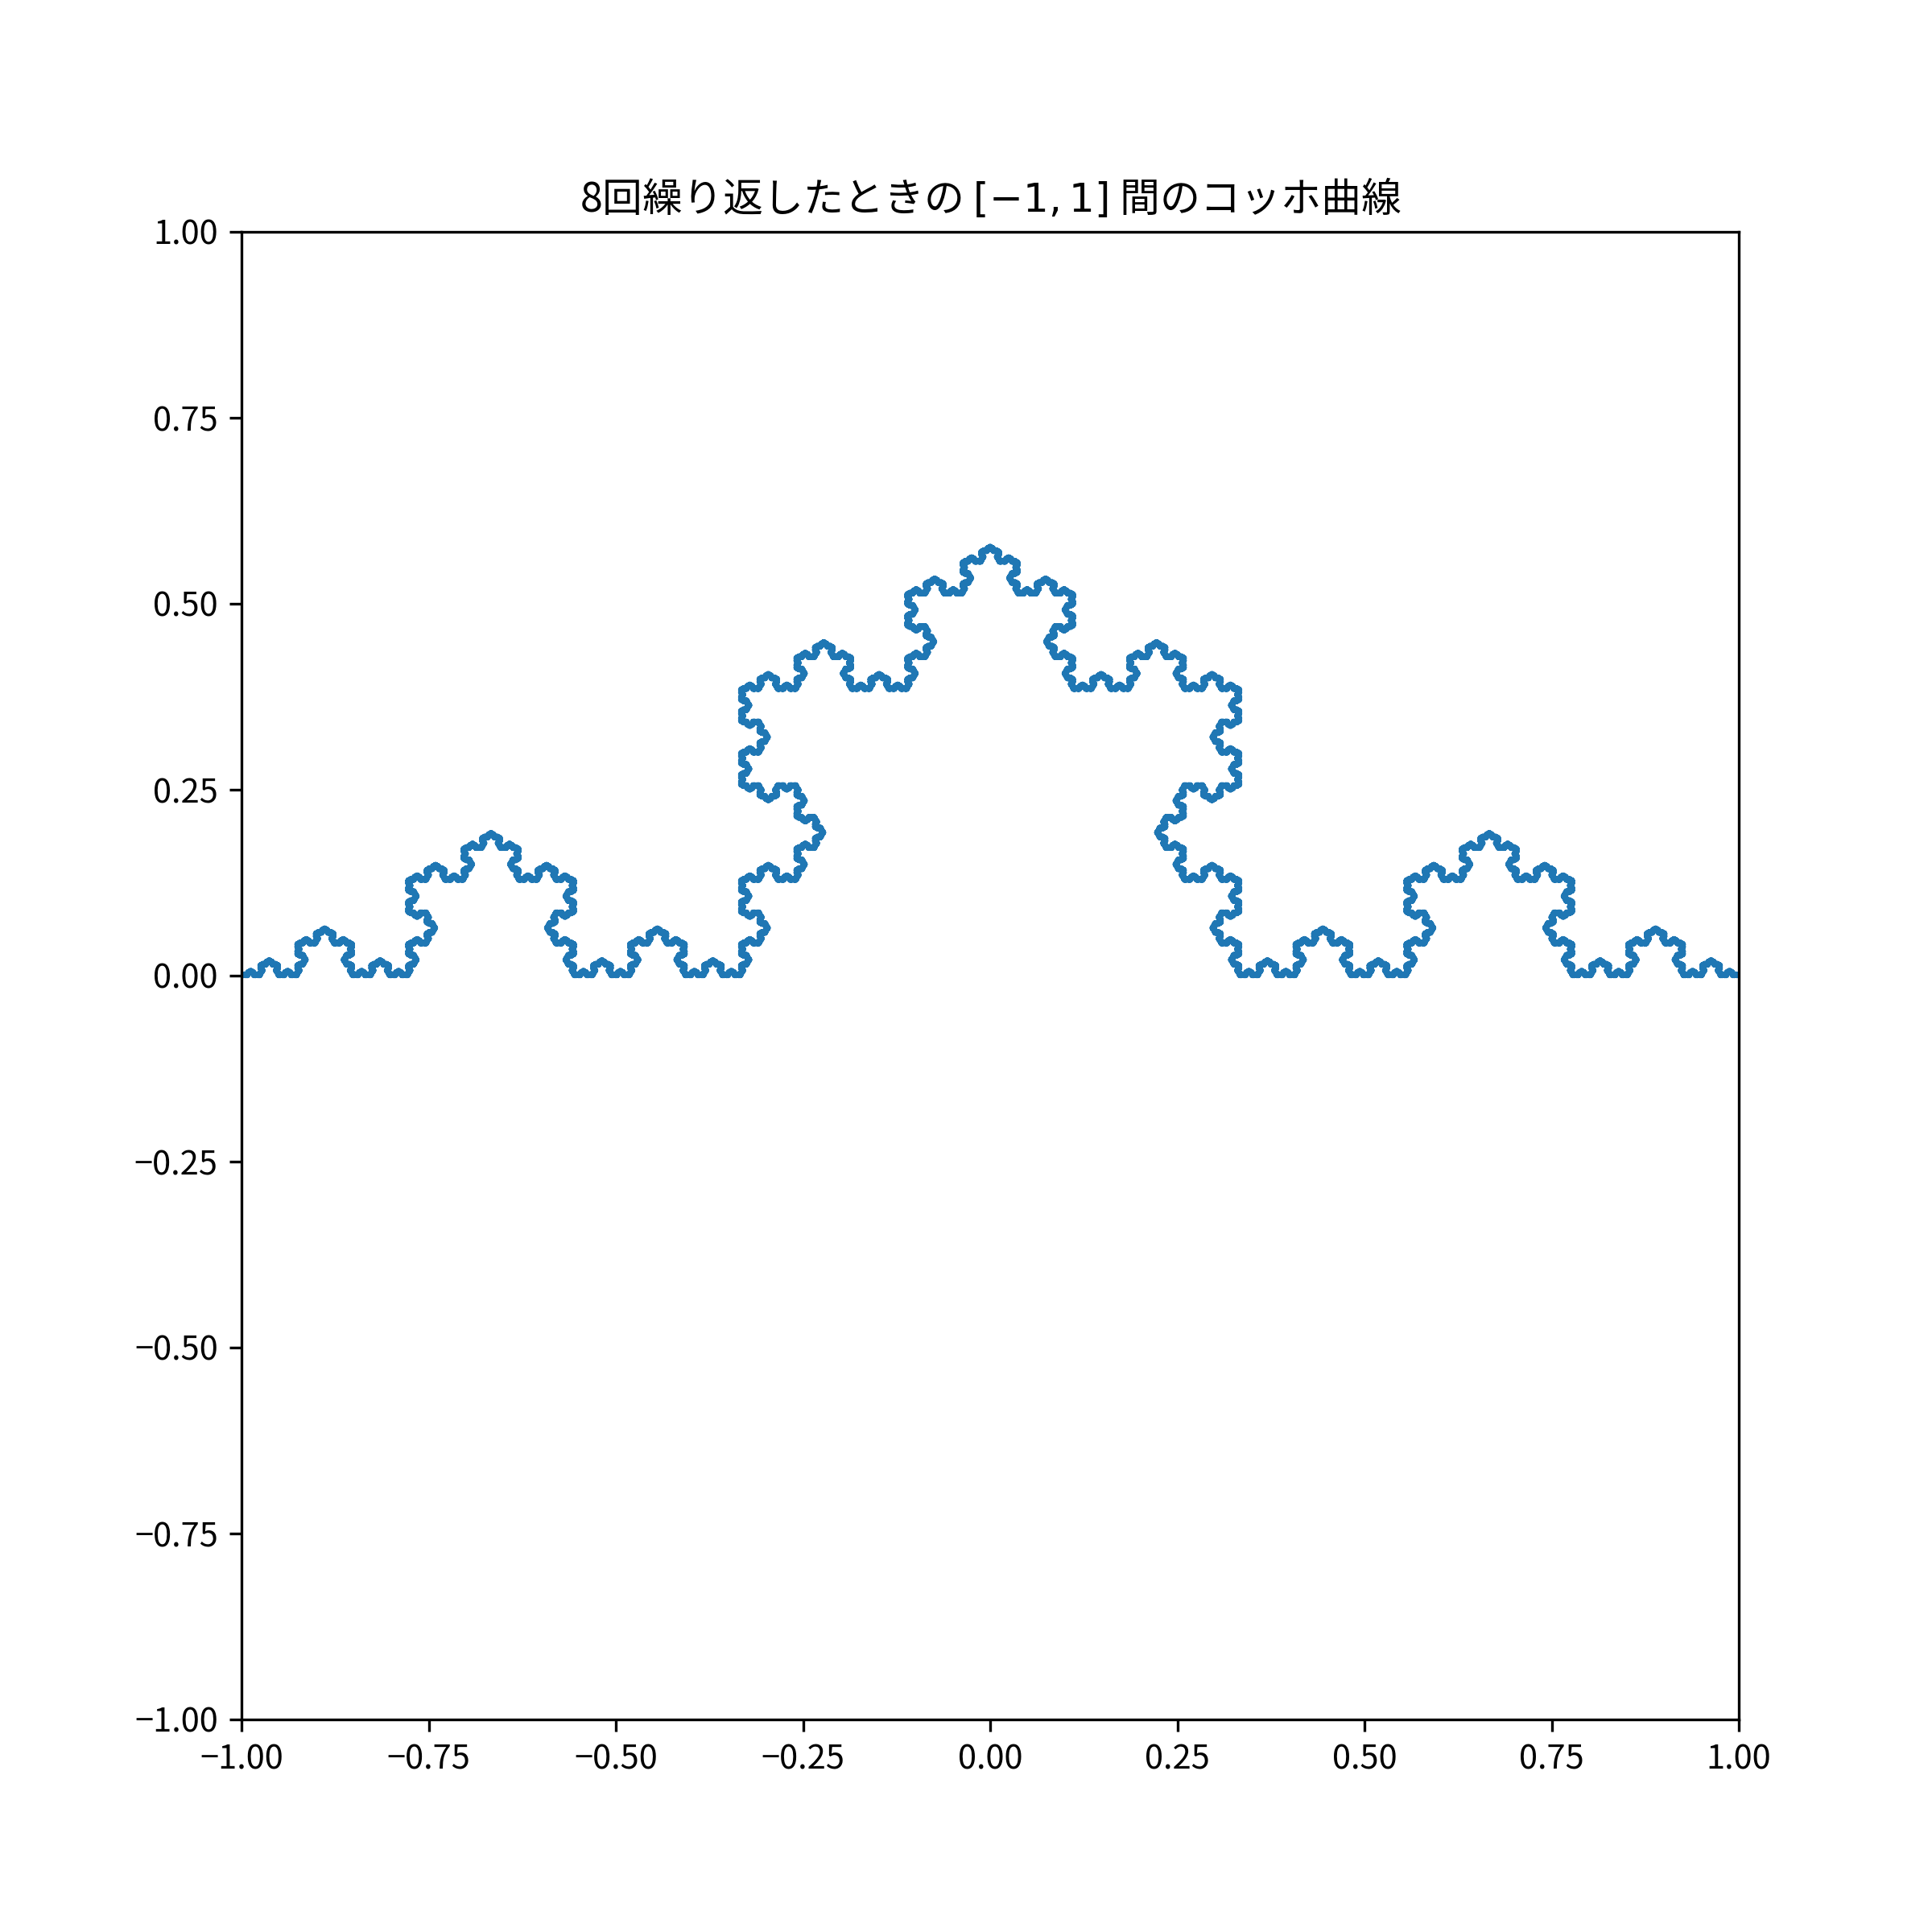
\includegraphics[keepaspectratio, scale=0.8]{images/OtherProblem/ctest5_3.png}
\end{figure}
解説:\\
このコッホ曲線を描くためのソースコードは、コッホ曲線の座標を任意の繰り返し回数で再帰し求める関数を作った。その座標の配列をもとにPythonのmatplotlibを用いてプロットした。\\
\begin{lstlisting}[caption=koch.py]
  import math
  import matplotlib
  from matplotlib import pyplot as plt
  import numpy as np

  # 日本語フォント用(Linux)
  matplotlib.rc('font', family='Noto Sans CJK JP')
  '''
  # 日本語フォント用(Windows)
  matplotlib.rc('font', family='MS Gothic')
  '''

  def koch(n: int, p1: list, p2: list) -> None:
      "再帰関数をもちいたコッホ曲線の座標を求める関数"
      if n == 0:
          return
      sx = 2 * p1[0] / 3 + p2[0] / 3
      sy = 2 * p1[1] / 3 + p2[1] / 3
      tx = p1[0] / 3 + 2 * p2[0] / 3
      ty = p1[1] / 3 + 2 * p2[1] / 3
      ux = (tx - sx) * math.cos(math.radians(60))  - (ty - sy) * math.sin(math.radians(60)) + sx
      uy = (tx - sx) * math.sin(math.radians(60)) + (ty - sy) * math.cos(math.radians(60)) + sy
      koch(n-1, p1, [sx, sy])
      # print(sx, sy)
      koch_array_x.append(sx)
      koch_array_y.append(sy)

      koch(n-1, [sx, sy], [ux, uy])
      # print(ux, uy)
      koch_array_x.append(ux)
      koch_array_y.append(uy)

      koch(n-1, [ux, uy], [tx, ty])
      # print(tx, ty)
      koch_array_x.append(tx)
      koch_array_y.append(ty)

      koch(n-1, [tx, ty], p2)

  n = 8
  p1 = [-1, 0]
  p2 = [1, 0]
  koch_array_x = [p1[0]]
  koch_array_y = [p1[1]]
  koch(n, p1, p2)
  koch_array_x.append(p2[0])
  koch_array_y.append(p2[1])
  file_path = "複雑系科学演習/Week6/images/"
  plt.figure(figsize=(8, 8))
  plt.title("{}回繰り返したときの $[-1, 1]$ 間のコッホ曲線".format(n))
  plt.xlim(-1, 1)
  plt.ylim(-1, 1)
  plt.plot(koch_array_x, koch_array_y)
  plt.savefig(file_path + "ctest5_3", dpi=300)
  plt.show()
\end{lstlisting}
\end{document}